\documentclass[a4paper, 12pt, openany]{book}

%\usepackage{blindtext} % needed for creating dummy text passages
%\usepackage[toc, page]{appendices}
%\usepackage{ngerman} % needed for German default language
\usepackage{amsmath} % needed for command eqref
\usepackage{amssymb} % needed for math fonts
\usepackage[utf8x]{inputenc}
\usepackage[greek, english]{babel}
%\usepackage{titlesec}
%\usepackage{xgreek}
%\usepackage{alphabeta}
\usepackage[
	colorlinks=true
	,breaklinks
	]{hyperref} % needed for creating hyperlinks in the document, the option colorlinks=true gets rid of the awful boxes, %breaklinks breaks lonkg links (list of figures), and ngerman sets everything for german as default hyperlinks% %language
\usepackage[hyphenbreaks]{breakurl} % benötigt für das Brechen von URLs in Literaturreferenzen, hyphenbreaks auch bei links, 
%die über eine Seite gehen (mit hyphenation).
\usepackage{xcolor}
\definecolor{c1}{rgb}{0,0,1} % blue
\definecolor{c2}{rgb}{0,0.3,0.9} % light blue
\definecolor{c3}{rgb}{0.3,0,0.9} % red blue
\hypersetup{
    linkcolor={c1}, % internal links
    citecolor={c2}, % citations
    urlcolor={c3} % external links/urls
}
\usepackage[noadjust]{cite} 		% needed for cite
%\usepackage[square, numbers]{natbib} 	% needed for cite and abbrvnat bibliography style
%\usepackage{iee}
\usepackage[nottoc]{tocbibind}		% needed for displaying bibliography and other in the table of contents
\usepackage{graphicx} 			% needed for \includegraphics 
\usepackage{longtable} 			% needed for long tables over pages
\usepackage{bigstrut} 			% needed for the command \bigstrut
\usepackage{enumerate} 			% needed for some options in enumerate
\usepackage{enumitem}
%\usepackage{todonotes} 		% needed for todos
%\usepackage{makeidx} % needed for creating an index
%\makeindex
\usepackage{algorithm, algcompatible}
\usepackage{empheq, nccmath}
\usepackage[numbers]{natbib} 	% needed for cite and abbrvnat bibliography style
\usepackage{setspace}
\usepackage{longtable}
\usepackage{booktabs}

\usepackage{colortbl}
\usepackage{acro}
\renewcommand{\thealgorithm}{}
\renewcommand{\arraystretch}{1.7}
\usepackage{changepage}
\usepackage{subcaption}
\acsetup{first-style=short, list-style=longtable, sort=false}
\algnewcommand\RETURN{\item[\textbf{return}]}
\setcounter{MaxMatrixCols}{17}
%\renewcommand\bibname{\textgreek{Βιβλιογραφία}}

%% page settings
%\usepackage[a4paper,width=130mm,top=35mm,bottom=40mm]{geometry}
\usepackage[top=2cm, bottom=1.8cm,left=2.5cm,right=2.5cm]{geometry} % needed for page border settings
%\usepackage{geometry}
\setlength{\parindent}{0em}% for space of first line of new text block
\setlength{\parskip}{1em}
\sloppy % for writing with hyphenless justification (tries to)
\hyphenation{} % use hyphenation of tolerance %parameters,http://www.jrx.de/publikationen/latex/tipps/zeilenumbruch.html
\hyphenpenalty=10000
\exhyphenpenalty=10000
\usepackage{fancyhdr} % needed for head and foot options
%\sectionfont{\bfseries\Large\raggedright}
\graphicspath{{Images/}}
\DeclareMathOperator*{\argmax}{argmax}
%\makeglossaries

%% my macros

%% Text fomats
\newcommand{\tbi}[1]{\textbf{\textit{#1}}}

%% Math fonts
\newcommand{\bbA}{\mathbb{A}}
\newcommand{\bbB}{\mathbb{B}}
\newcommand{\bbC}{\mathbb{C}}
\newcommand{\bbD}{\mathbb{D}}
\newcommand{\bbE}{\mathbb{E}}
\newcommand{\bbF}{\mathbb{F}}
\newcommand{\bbG}{\mathbb{G}}
\newcommand{\bbH}{\mathbb{H}}
\newcommand{\bbI}{\mathbb{I}}
\newcommand{\bbJ}{\mathbb{J}}
\newcommand{\bbK}{\mathbb{K}}
\newcommand{\bbL}{\mathbb{L}}
\newcommand{\bbM}{\mathbb{M}}
\newcommand{\bbN}{\mathbb{N}}
\newcommand{\bbO}{\mathbb{O}}
\newcommand{\bbP}{\mathbb{P}}
\newcommand{\bbQ}{\mathbb{Q}}
\newcommand{\bbR}{\mathbb{R}}
\newcommand{\bbS}{\mathbb{S}}
\newcommand{\bbT}{\mathbb{T}}
\newcommand{\bbU}{\mathbb{U}}
\newcommand{\bbV}{\mathbb{V}}
\newcommand{\bbW}{\mathbb{W}}
\newcommand{\bbX}{\mathbb{X}}
\newcommand{\bbY}{\mathbb{Y}}
\newcommand{\bbZ}{\mathbb{Z}}
% abbreviations:
\DeclareAcronym{cnn}{
  short = \textbf{CNN} ,
  long  = \textbf{C}onvolutional \textbf{N}eural \textbf{N}etwork,
  class = abbrev}

  \DeclareAcronym{fcnn}{
  short = \textbf{FCNN} ,
  long  = \textbf{F}ully \textbf{C}onvolutional \textbf{N}eural \textbf{N}etwork,
  class = abbrev}
  
\DeclareAcronym{rnn}{
  short = \textbf{RNN} ,
  long  = \textbf{R}ecurrent \textbf{N}eural \textbf{N}etwork,
  class = abbrev}
  
\DeclareAcronym{nn}{
  short = \textbf{NN} ,
  long  = \textbf{N}eural \textbf{N}etwork,
  class = abbrev}
  
  \DeclareAcronym{mrf}{
  short = \textbf{MRF} ,
  long  = \textbf{M}arkov \textbf{R}andom \textbf{F}ield,
  class = abbrev}

\DeclareAcronym{crf}{
  short = \textbf{CRF},
  long  = \textbf{C}onditional \textbf{R}andom \textbf{F}ield,
  class = abbrev}  

\DeclareAcronym{crf-rnn}{
  short = \textbf{CRF-RNN},
  long  = \textbf{C}onditional \textbf{R}andom \textbf{F}ield as \textbf{R}ecurrent \textbf{N}eural \textbf{N}etwork,
  class = abbrev}

\DeclareAcronym{nn-gr}{
  short = \textgreek{\textbf{ΝΔ}} ,
  long  = \textgreek{\textbf{Ν}ευρωνικό \textbf{Δ}ίκτυο},
  class = abbrev}
\DeclareAcronym{crf-gr}{
  short = \textgreek{\textbf{ΤΥΣΠ}},
  long  = \textgreek{\textbf{Τ}υχαίο \textbf{Υ}πό \textbf{Σ}υνθήκη \textbf{Π}εδίο},
  class = abbrev}
  
\DeclareAcronym{crf-rnn-gr}{
  short = \textgreek{\textbf{ΤΥΣΠ-ΕΝΔ}},
  long  = \textgreek{\textbf{Τ}υχαίο \textbf{Υ}πό \textbf{Σ}υνθήκη \textbf{Π}εδίο ως \textbf{Ε}παναλαμβανόμενο \textbf{Ν}ευρωνικό \textbf{Δ}ίκτυο},
  class = abbrev}  
  
\DeclareAcronym{cnn-gr}{
  short = \textgreek{\textbf{ΣΝΔ}},
  long  = \textgreek{\textbf{Σ}υνελικτικό \textbf{Ν}ευρωνικό \textbf{Δ}ίκτυο},
  class = abbrev}
  
\DeclareAcronym{fcnn-gr}{
  short = \textgreek{\textbf{ΠΣΝΔ}} ,
  long  = \textgreek{\textbf{Π}λήρως \textbf{Σ}υνελικτικό \textbf{Ν}ευρωνικό \textbf{Δ}ίκτυο},
  class = abbrev}
  
\DeclareAcronym{rnn-gr}{
  short = \textgreek{\textbf{ENΔ}},
  long  = \textgreek{\textbf{Ε}παναλαμβανόμενο \textbf{Ν}ευρωνικό \textbf{Δ}ίκτυο},
  class = abbrev}
\addto\captionsenglish{
  \renewcommand{\figurename}{\textgreek{Εικόνα}}
  \renewcommand{\contentsname}{\textgreek{Περιεχόμενα}}
  \renewcommand{\tablename}{\textgreek{Πίνακας}}
  \renewcommand{\bibname}{\textgreek{Βιβλιογραφία}}
  \renewcommand{\listfigurename}{\textgreek{Κατάλογος Εικόνων}}
  \renewcommand{\listtablename}{\textgreek{Κατάλογος Πινάκων}}
  \renewcommand{\chaptername}{\textgreek{Κεφάλαιο}}
}

\bibliographystyle{abbrvnat}

% Main document Below
\begin{document}
\acuseall

\pagestyle{empty}
%%%%%%%%%%%%%%%%%%%%%%%%%%%%%%%%%%%%%%%%%
% University Assignment Title Page 
% LaTeX Template
% Version 1.0 (27/12/12)
%
% This template has been downloaded from:
% http://www.LaTeXTemplates.com
%
% Original author:
% WikiBooks (http://en.wikibooks.org/wiki/LaTeX/Title_Creation)
%
% License:
% CC BY-NC-SA 3.0 (http://creativecommons.org/licenses/by-nc-sa/3.0/)
% 
% Instructions for using this template:
% This title page is capable of being compiled as is. This is not useful for 
% including it in another document. To do this, you have two options: 
%
% 1) Copy/paste everything between \begin{document} and \end{document} 
% starting at \begin{titlepage} and paste this into another LaTeX file where you 
% want your title page.
% OR
% 2) Remove everything outside the \begin{titlepage} and \end{titlepage} and 
% move this file to the same directory as the LaTeX file you wish to add it to. 
% Then add \input{./title_page_1.tex} to your LaTeX file where you want your
% title page.
%
%%%%%%%%%%%%%%%%%%%%%%%%%%%%%%%%%%%%%%%%%

%----------------------------------------------------------------------------------------
%	PACKAGES AND OTHER DOCUMENT CONFIGURATIONS
%----------------------------------------------------------------------------------------

%\documentclass[12pt]{article}
%
%\begin{document}

\begin{titlepage}
%\SetDate[01/01/2016]
\newcommand{\HRule}{\rule{\linewidth}{0.5mm}} % Defines a new command for the horizontal lines, change thickness here

\center % Center everything on the page
 
%----------------------------------------------------------------------------------------
%	HEADING SECTIONS
%----------------------------------------------------------------------------------------

\textsc{\LARGE University of Thessaly}\\[1.5cm] % Name of your university/college
\textsc{\Large Department of Electrical and \\ Computer Engineering}\\[0.5cm] % Major heading such as course name
\textsc{\large DIPLOMA THESIS}\\[0.5cm] % Minor heading such as course title

%----------------------------------------------------------------------------------------
%	TITLE SECTION
%----------------------------------------------------------------------------------------

\HRule \\[0.4cm]
{ \huge \bfseries Semantics Segmentation of Urban Environment Images}\\[0.4cm] % Title of your document
\HRule \\[1.5cm]
 
%----------------------------------------------------------------------------------------
%	AUTHOR SECTION
%----------------------------------------------------------------------------------------

\begin{minipage}{0.4\textwidth}
\begin{flushleft} \large
\emph{Author:}\\
Dimitrios Mallios % Your name
\end{flushleft}
\end{minipage}
~
\begin{minipage}{0.4\textwidth}
\begin{flushright} \large
\emph{Supervisors:} \\
Gerasimos Potamianos \\
Antonios Argyriou % Supervisor's Name
\end{flushright}
\end{minipage}\\[4cm]

% If you don't want a supervisor, uncomment the two lines below and remove the section above
%\Large \emph{Author:}\\
%John \textsc{Smith}\\[3cm] % Your name

%----------------------------------------------------------------------------------------
%	DATE SECTION
%----------------------------------------------------------------------------------------
%
{\large June 27, 2018}\\[3cm] % Date, change the \today to a set date if you want to be precise

%----------------------------------------------------------------------------------------
%	LOGO SECTION
%----------------------------------------------------------------------------------------


\includegraphics[width=0.2\textwidth]{Images/uth_logo}\\[1cm] % Include a department/university logo - this will require the graphicx package
 
%----------------------------------------------------------------------------------------

\vfill % Fill the rest of the page with whitespace

%%%%%%%%%%%%%%%%%%%%%%%%%%%%%%%%%%%%%%%%%%%%%%%%%%%%%%%%%%%%%%%%%%%%%%%%%%%%%%%%%
%%%%%%%%%%%%%%%%%%%%%%%%%%%%%%%%%%%% GREEK PART %%%%%%%%%%%%%%%%%%%%%%%%%%%%%%%%%
%%%%%%%%%%%%%%%%%%%%%%%%%%%%%%%%%%%%%%%%%%%%%%%%%%%%%%%%%%%%%%%%%%%%%%%%%%%%%%%%%

\newpage
\center % Center everything on the page
 
%----------------------------------------------------------------------------------------
%	HEADING SECTIONS
%----------------------------------------------------------------------------------------
\textsc{\LARGE \textgreek{ΠΑΝΕΠΙΣΤΗΜΙΟ ΘΕΣΣΑΛΙΑΣ}}\\[1.5cm] % Name of your university/college
\textsc{\Large \textgreek{Τμήμα Ηλεκτρολόγων Μηχανικών και \\ Μηχανικών Η/Υ}}\\[0.5cm] % Major heading such as course name
\textsc{\large \textgreek{ΔΙΠΛΩΜΑΤΙΚΗ ΕΡΓΑΣΙΑ}}\\[0.5cm] % Minor heading such as course title

%----------------------------------------------------------------------------------------
%	TITLE SECTION
%----------------------------------------------------------------------------------------

\HRule \\[0.4cm]
{ \huge \bfseries \textgreek{Σημασιολογική Κατάτμηση Εικόνων Αστικού Περιβάλλοντος}}\\[0.4cm] % Title of your document
\HRule \\[1.5cm]
 
%----------------------------------------------------------------------------------------
%	AUTHOR SECTION
%----------------------------------------------------------------------------------------

\begin{minipage}{0.4\textwidth}
\begin{flushleft} \large
\emph{\textgreek{Συγγραφέας}:}\\
\textgreek{Δημήτριος Μάλλιος} % Your name
\end{flushleft}
\end{minipage}
~
\begin{minipage}{0.4\textwidth}
\begin{flushright} \large
\emph{\textgreek{Επιβλέποντες}:} \\
\textgreek{Γεράσιμος Ποταμιάνος\\
Αντώνιος Αργυρίου}

\end{flushright}
\end{minipage}\\[4cm]

% If you don't want a supervisor, uncomment the two lines below and remove the section above
%\Large \emph{Author:}\\
%John \textsc{Smith}\\[3cm] % Your name

%----------------------------------------------------------------------------------------
%	DATE SECTION
%----------------------------------------------------------------------------------------

%{\large \today}\\[3cm] % Date, change the \today to a set date if you want to be precise

%----------------------------------------------------------------------------------------
%	LOGO SECTION
%----------------------------------------------------------------------------------------


\includegraphics[width=0.2\textwidth]{Images/uth_logo}\\[1cm] % Include a department/university logo - this will require the graphicx package
 
%----------------------------------------------------------------------------------------

\vfill % Fill the rest of the page with whitespace

\end{titlepage}
%\end{document} 
\chapter*{\centering \textgreek{\emph{Περίληψη}}}
%\addtocontents{toc}{\protect\contentsline{chapter}{\protect\numberline{}\textgreek{Περίληψη (Ελληνικά)}}{}{chapter*.%\thepage}}
%\addcontentsline{toc}{chapter}{Abstract (Greek)}
\textgreek{Η παρούσα διπλωματική εξετάζει το πρόβλημα της αναγνώρισης αντικειμένων από εικόνες, των οποίων τα εικονοστοιχεία είναι ταξινομημένα σε μια από 19 κατηγορίες. Στην εργασία χρησιμοποιείται η βάση δεδομένων} Cityscapes\textgreek{ που αποτελείται από 19 διαφορετικές κατηγορίες αντικειμένων η οποία έχει δημιουργηθεί με χρήση κάμερας τοποθετημένη στο εμπρόσθιο μέρος αυτοκινήτου. Οι εικόνες έχουν απαθανατιστεί από 50 διαφορετικές πόλεις της Ευρώπης σε διάφορες εποχές και καιρικές συνθήκες. \par 

Με την χρήση πληροφορίας από έγχρωμες εικόνες κατασκευάζουμε έναν ταξινομητή ο οποίος μπορεί να αναγνωρίσει την κατηγορία αντικειμένων που ανήκει το κάθε εικονοστοιχείο στην εικόνα ως συνάρτηση των τιμών των εικονοστοιχείων αλλά και της δομής που απεικονίζουν. Για την ταξινόμηση χρησιμοποιήσαμε 2 πανομοιότυπες αρχιτεκτονικές πλήρως συνελικτικών νευρωνικών δικτύων (}FCNNs\textgreek{) και 2 διαφορετικές μονάδες μετα-επεξεργασίας.} \par

\textgreek{Στόχος της εργασίας ήταν η δημιουργία διαφορετικών ταξινομητών καθώς και η σύγκριση μεταξύ των μεθόδων, αλλά και η δημιουργία λογισμικού για την οπτικοποίηση των αποτελεσμάτων. Για την οπτικοποίηση των παραπάνω αποτελεσμάτων υλοποιήθηκε λογισμικό που απεικονίζει τα αποτελέσματα των μεθόδων. Για την κατασκευή των παραπάνω μοντέλων γίνεται χρήση των βιβλιοθηκών } Keras \textgreek{ και} Tensorflow, \textgreek{ ενώ για την υλοποίηση του λογισμικού οπτικοποίησης έγινε η χρήση της βιβλιοθήκης} pyQt.
 

\chapter*{\centering \emph{Abstract}}
%\addtocontents{toc}{\protect\contentsline{chapter}{\protect\numberline{}Abstract (English)}{}{chapter*.\thepage}}

This thesis focuses on the problem of recognizing objects from images which are pixel-wise classified in one of 19 various classes. The Cityscapes database introduced in CVPR 2016, consists of 19 various classes of objects created using a camera mounted on automobiles. Images have been recorded in 50 European cities in different seasons and weather conditions.
\par 
Using information from coloured images, a classifier was implemented to recognize the category of objects where each individual pixel belongs to. As part of classification, two different Fully Convolutional Neural Networks models along with another two post processing units were implemented. 
\par 

The aim of this thesis is to create and compare the results from various model architectures, and to also integrate a sophisticated visualizer which presents their results. The tools used in this project are Keras and Tensorflow, as well as pyQt for the implementation of the visualizer.

\chapter*{\centering\emph{\textgreek{Ευχαριστίες}}}
\textgreek{Θα ήθελα να ευχαριστήσω τους επιβλέποντες καθηγητές μου, καθηγητές Γεράσιμο Ποταμιάνο και Αντώνιο Αργυρίου για την υποστήριξη αλλά και την απαραίτητη γνώση και τα κίνητρα που μου έδωσαν μέσα από τα μαθήματα τους ώστε να πραγματοποιηθεί αυτή η διπλωματική. Επίσης, θα ήθελα να ευχαριστήσω τον συνεπιβλέποντα ερευνητή Θεόδωρο Γιαννακόπουλο από το Ε.Κ.Ε.Φ.Ε Δημόκριτος για την υποστήριξη καθώς και τους ανθρώπους από το εργαστήριο Υπολογιστικής Ευφυΐας που μου έδωσαν χώρο και πόρους για να υλοποιηθεί αυτή η διπλωματική.}

%\input{abstractEn}

%\pagestyle{plain}
%\setotherlanguage{greek}
%\selectlanguage{greek}
\listoffigures
\listoftables
%\listofalgorithms
\tableofcontents
\raggedbottom


\pagebreak
%\printglossary[type=\acronymtype,title=Abbreviations]
% Insert dedication
%\vspace*{10cm}
%\centering{\large{\emph{\textgreek{ Στην Οικογενειά μου...} }}}
%\vfill
\begin{center}
\topskip0pt
\vspace*{\fill}
 \large{\emph{\textgreek{Στην Οικογένειά μου...}}} 
\vspace*{\fill}
\end{center}

\pagebreak
%\raggedright ???
%%%%%%%% Abbrevations %%%%%
%\cleardoublepage
\printacronyms[include-classes=abbrev, name=\huge \textgreek{Ακρωνύμια}]
%\raggedcenter
%\pagestyle{plain}

\chapter{\textgreek{Εισαγωγή}}
\label{chapter_1}
%\pagestyle{empty}
\pagestyle{fancy}
\fancyhf{}
%\fancyhead[OC]{\leftmark}
%\fancyhead[C]{}
%\fancyhead[EC]{\rightmark}
\renewcommand{\footrulewidth}{0.5pt}
\cfoot{\thepage}

%\begin{flushleft}

\section{\textgreek{Μηχανική Μάθηση και Σημασιολογική Κατάτμηση}}
\textgreek{Μηχανική Μάθηση είναι ένας τομέας ο οποίος ανήκει στην Επιστήμη των Υπολογιστών ο οποίος επικεντρώνεται σε εκλεπτυσμένους αλγορίθμους οι οποίοι δεν έχουν δημιουργηθεί ρητά από τους επιστήμονες, αλλά μαθαίνουν από τα δεδομένα και προσαρμόζονται σε αυτά για να κάνουν προβλέψεις ή για να πάρουν αποφάσεις. Τα τελευταία χρόνια η εξέλιξη της υπολογιστικής δύναμης καθώς και ο μεγάλος όγκος δεδομένων που είναι διαθέσιμος επιτρέπει στους επιστήμονες να πειραματιστούν με πιο πολύπλοκους αλγόριθμους. Ο συγκεκριμένος κλάδος καλύπτει ένα μεγάλο εύρος εφαρμογών, από μηχανές αναζήτησης} [\citenum{7538344}]\textgreek{ και μετάφραση κειμένου }\cite{machine_translation}\textgreek{ μέχρι εκτιμήσεις για ασθένειες στον κλάδο της Ιατρικής} \cite{medical_pred}.

% Σε αυτή την εργασία, αποφασίσαμε να επικεντρωθούμε στο θέμα της Σημασιολογικής Κατάτμησης από εικόνες αστικών περιοχών.
%\subsubsection{Data and Description}
%\lhead{}
\section{\textgreek{Σημασιολογική Κατάτμηση και Αναγνώριση Αντικειμένων}}
\textgreek{Στην Επιστήμη των Υπολογιστών υπάρχει μια διαφοροποιήση μεταξύ ενός προβλήματος αναγνώρισης αντικειμένων και ενός προβλήματος Σημασιολογικής Κατάτμησης αντικειμένων. Αυτά τα δύο προβλήματα ενώ στην ουσία αποσκοπούν στον ίδιο στόχο, έχουν μια πολύ σημαντική διαφορά. Όταν μιλάμε για αναγνώριση αντικειμένων δεν αναφερόμαστε στην ακριβή εύρεση της τοποθεσίας ενός αντικειμένου στην εικόνα αλλά στη γενική του μορφή, δηλαδή χωρίς την ακριβή εύρεση των ορίων του αντικειμένου (εικόνα} \ref{fig:yolo_img}). \textgreek{Εν αντιθέσει, στο θέμα της Σημασιολογικής Κατάτμησης αντικειμένων, μας ενδιαφέρει η τοποθεσία ενός αντικειμένου στην εικόνα αλλά και η εύρεση των ακριβών ορίων του αντικειμένου, καθώς τοποθετούμε κάθε εικονοστοιχείο της εικόνας σε μια κατηγορία αντικειμένου (εικόνα} \ref{fig:seg_img}). \\[2cm] \textgreek{Στις παρακάτω εικόνες φαίνονται ξεκάθαρα οι διαφορές των 2 προβλημάτων.}

\begin{figure}[h!]
\centering
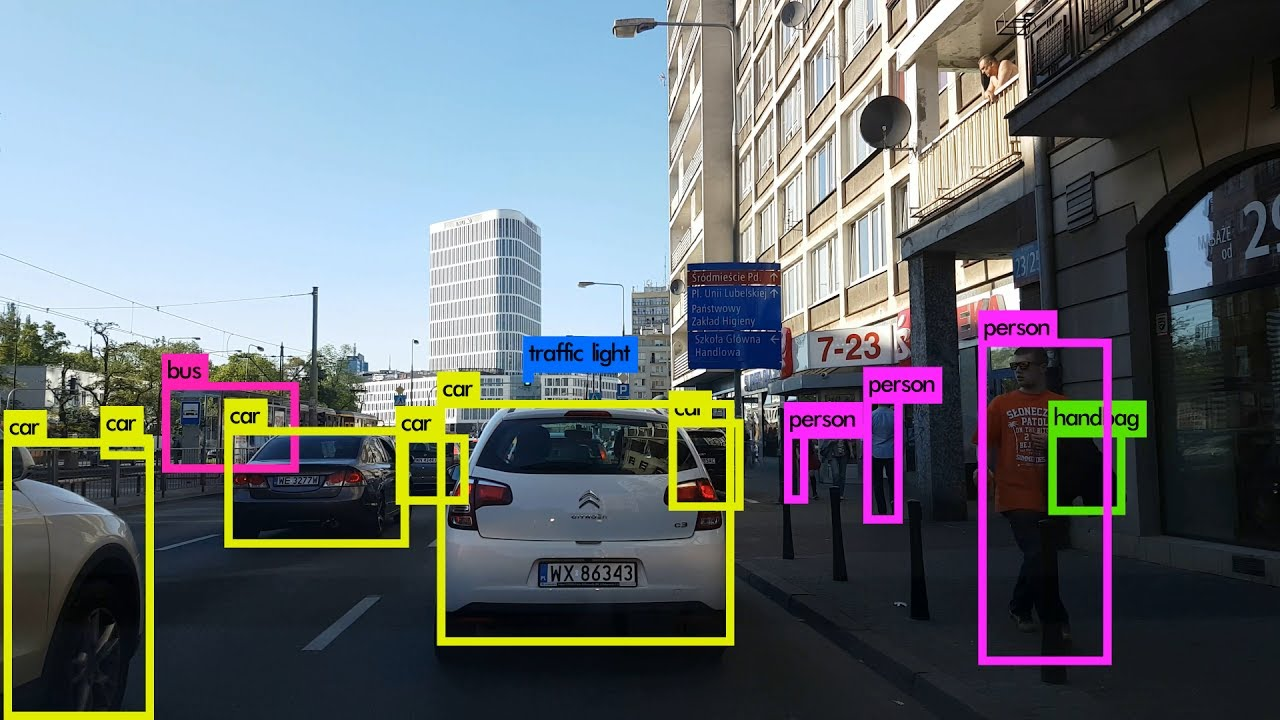
\includegraphics[scale=0.3]{Images/Obj_det}
\caption[\textgreek{Αναγνώριση} YOLO]{\textgreek{Παράδειγμα ενός συστήματος αναγνώρισης αντικειμένων. Αποτέλεσμα του συστήματος }YOLO \cite{yolo}}
\label{fig:yolo_img}
\end{figure}

\begin{figure}[h!]
\centering
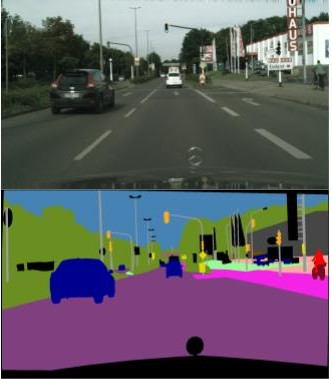
\includegraphics{Images/seg}
\caption[\textgreek{Παράδειγμα Σημασιολογίας}]{\textgreek{Παράδειγμα ενός συστήματος Σημασιολογικής Κατάτμησης αντικειμένων από εικόνες.}}
\label{fig:seg_img}
\end{figure}

\section{\textgreek{Η Βάση Δεδομένων} Cityscapes }
\textgreek{Σε αυτή την εργασία χρησιμοποιήθηκε η βάση δεδομένων} \href{https://www.cityscapes-dataset.com/} {Cityscapes} \cite{Cityscapes} \textgreek{η οποία αποτελείται από ένα σύνολο έγχρωμων εικόνων υψηλής ευκρίνειας τραβηγμένες σε αστικές περιοχές. Περιλαμβάνει 19 κατηγορίες αντικειμένων ενώ διαθέτει και μία επιπλέον κατηγορία για την ταξινόμηση των αντικειμένων που δεν ανήκουν σε καμία κατηγορία. Τα αντικείμενα στις εικόνες έχουν επισημειωθεί σε επίπεδο εικονοστοιχείου. Δηλαδή, όλα τα εικονοστοιχεία της εικόνας ανήκουν σε κάποιο αντικείμενο. Η βάση περιέχει περισσότερες από 5000 εικόνες μεγέθους 1024}x\textgreek{2048 εικονοστοιχείων από 50 πόλεις της Ευρώπης. Οι εικόνες έχουν τραβηχτεί από μια κάμερα ακολουθιακά με διάστημα ενός δευτερολέπτου μεταξύ τους.}
\\[1cm]
\textgreek{Το σύνολο δεδομένων διαθέτει επίσης ένα άλλο κομμάτι το οποίο αποτελείται από 20000 εικόνες των οποίων τα εικονοστοιχεία έχουν επισημειωθεί πιο αφηρημένα. Οι παρακάτω εικόνες δείχνουν τη διαφορά μεταξύ των δύο συνόλων, οι μερικώς επισημειωμένες εικόνες δεν έχουν όλα τα εικονοστοιχεία ταξινομημένα. Το συγκεκριμένο σύνολο από εικόνες δεν έχει χρησιμοποιηθεί στα πειράματά μας.}

\begin{figure}[h!]
 \centering
 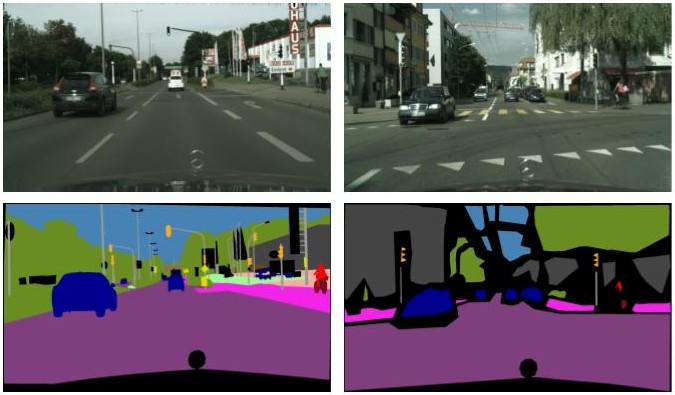
\includegraphics[scale=0.6]{Images/dataset.jpg}
 \caption[\textgreek{Παράδειγμα Εικόνων Βάσης}]{\textgreek{Αριστερά: Πλήρως επισημειωμένες εικόνες.
 \\ Εικόνα Δεξιά: Μερικώς επισημειωμένες εικόνες.}}
\end{figure}


%\{Semantics Segmentation Applications}

\subsection{\textgreek{Περιγραφή Αντικειμένων}}
\textgreek{Η βάση περιέχει 19 αντικείμενα τα οποία ανήκουν σε 6 υπερ-κατηγορίες. Τα εικονοστοιχεία που ανήκουν σε κατηγορίες αντικειμένων που δεν μας αφορούν στην διαδικασία της αναγνώρισης είναι σημειωμένα ως} \emph{\textgreek{`Χωρίς Ετικέτα`}}. \textgreek{Αυτά τα αντικείμενα πιο αναλυτικά είναι:}
\\[1cm]
\[
\begin{array}{lccc}
 \text{Classes} &\text{\textgreek{Κλάσεις}} & \text{Categories} &\text{\textgreek{Κατηγορίες}}\\
 \hline
 
 \text{Road} 		&\text{\textgreek{Δρόμος}} & 	\text{Flat} &\text{\textgreek{Επίπεδο}}\\
 \text{Sidewalk} 	&\text{\textgreek{Πεζοδρόμιο}} & \text{Flat} &\text{\textgreek{Επίπεδο}}\\
 \text{Building} 	&\text{\textgreek{Κτίριο}} & 	\text{Construction} &\text{\textgreek{Κατασκευή}}\\
 \text{Wall} 		&\text{\textgreek{Τοίχος}} & 	\text{Construction} &\text{\textgreek{Κατασκευή}}\\
 \text{Fence} 		&\text{\textgreek{Φράχτης}} & 	\text{Construction} &\text{\textgreek{Κατασκευή}}\\
 \text{Pole} 		&\text{\textgreek{Ιστός}} & 	\text{Object} &\text{\textgreek{Αντικείμενο}}\\
 \text{Traffic light} 	&\text{\textgreek{Φανάρι κυκλοφορίας}} & \text{Object} &\text{\textgreek{Αντικείμενο}}\\
 \text{Traffic sign} 	&\text{\textgreek{Πινακίδα κυκλοφορίας}} & \text{Object} &\text{\textgreek{Αντικείμενο}}\\
 \text{Vegetation} 	&\text{\textgreek{Βλάστηση}} & 		\text{Nature} &\text{\textgreek{Φύση}}\\
 \text{Terrain} 	&\text{\textgreek{Έδαφος}} & 		\text{Nature} &\text{\textgreek{Κατηγορίες}}\\
 \text{Sky} 		&\text{\textgreek{Ουρανός}} & 		\text{Sky} &\text{\textgreek{Ουρανός}}\\
 \text{Person} 		&\text{\textgreek{Άνθρωπος}} &		\text{Human} &\text{\textgreek{Άνθρωπος}}\\
 \text{Rider} 		&\text{\textgreek{Αναβάτης}} & 		\text{Human} &\text{\textgreek{Άνθρωπος}}\\
 \text{Car} 		&\text{\textgreek{Αυτοκίνητο}} & 	\text{Vehicle} &\text{\textgreek{Όχημα}}\\
 \text{Truck} 		&\text{\textgreek{Φορτηγό}} & 		\text{Vehicle} &\text{\textgreek{Όχημα}}\\
 \text{Bus} 		&\text{\textgreek{Λεωφορείο}} & 	\text{Vehicle} &\text{\textgreek{Όχημα}}\\
 \text{Train} 		&\text{\textgreek{Τρένο}} & 		\text{Vehicle} &\text{\textgreek{Όχημα}}\\
 \text{Motorcycle} 	&\text{\textgreek{Μοτοσυκλέτα}} & 	\text{Vehicle} &\text{\textgreek{Όχημα}}\\
 \text{Bicycle} 	&\text{\textgreek{Ποδήλατο}} & 		\text{Vehicle} &\text{\textgreek{Όχημα}}\\
 \text{Unlabeld} 	&\text{\textgreek{Χωρίς Ετικέτα}} & 	\text{Void} &\text{\textgreek{Κενό}}\\
  \hline
\end{array}
\]
%

\section{\textgreek{Με μια Ματιά}}
\subsection{\textgreek{Στόχοι Διπλωματικής}}
\textgreek{Ο σκοπός αυτής της Διπλωματικής είναι να μελετήσουμε το πρόβλημα της Σημασιολογικής Κατάτμησης Έγχρωμων Εικόνων οι οποίες αναπαριστούν αστικά περιβάλλοντα με την χρήση μεθόδων μηχανικής μάθησης. Η προσπάθειά μας στοχεύει στην πλήρη και ολοκληρωμένη ανασκόπηση ορισμένων από τους αλγορίθμους και τα εργαλεία που θα μπορούσαν να χρησιμοποιηθούν σε αυτόν τον συγκεκριμένο τομέα καθώς και στη σύγκριση των διαφόρων μεθόδων ταξινόμησης. Η δουλειά μας βασίζεται στην έρευνα που δημοσιεύτηκε στον ιστότοπο του }Cityscapes-Dataset \textgreek{προκειμένου να αποκτηθούν γνώσεις στον τομέα και ως εκ τούτου να επεκτείνουμε αυτή την έρευνα με τις δικές μας συνεισφορές.}

\subsection{\textgreek{Συνεισφορά της Διπλωματικής}}
\textgreek{Η Σημασιολογική Κατάτμηση πληροφορίας από εικόνες είναι ο τομέας ο οποίος στοχεύει να αλλάξει τον τρόπο με τον οποίο οι μηχανές αντιλαμβάνονται τον κόσμο. Συγκεκριμένα, υπάγεται στον κλάδο της Όρασης Υπολογιστών και αποσκοπεί στο να δώσουμε την ικανότητα στις μηχανές να μπορούν να αναγνωρίζουν τα αντικείμενα με λεπτομερή ακρίβεια, δηλαδή την τμηματοποίηση των αντικειμένων σε σχέση με το υπόβαθρο αλλά και μεταξύ των υπολοίπων αντικειμένων διαγράφοντας με λεπτομέρεια τα όρια των αντικειμένων. Αυτή η πτυχιακή παρουσιάζει μία επισκόπηση του κλάδου της Σημασιολογικής Κατάτμησης πληροφορίας από εικόνες αστικών περιοχών αλλά και στην περαιτέρω έρευνα του προβλήματος. Μέσα από την έρευνα και των μεθόδων και των αλγορίθμων που χρειάζονται, παρέχουμε τις δικές μας λύσεις αλλά και συγκρίσεις μεταξύ των μεθόδων που πειραματιστήκαμε. Για την οπτικοποίηση των αποτελεσμάτων προχωρήσαμε στην υλοποίηση της πλατφόρμας που μας δείχνει διαισθητικά τα αποτελέσματα των μεθόδων.\\

Εν ολίγοις οι συνεισφορές της εργασίας μπορούν να συνοψιστούν ως εξής}:

\begin{description}[labelindent=0.5cm, style=multiline, leftmargin=1cm, font=$\bullet$~]
 \item \textgreek{Στην περαιτέρω έρευνα στον τομέα της Σημασιολογικής Κατάτμησης Αντικειμένων από Εικόνες.}
 \item \textgreek{Στην σύγκριση των αποτελεσμάτων μεταξύ των μεθόδων που πειραματιστήκαμε πάνω σε ένα αληθινό πρόβλημα με την χρήση της βάση δεδομένων} Cityscapes-Dataset.
 \item \textgreek{Στην χρήση των σύγχονων εργαλείων }Keras, Tensorflow, OpenCV \textgreek{και} pyQt.
\end{description}


\subsection{\textgreek{Δομή της Διπλωματικής}}
\textgreek{Η Διπλωματική αποτελείται από 5 κεφάλαια, όπου το καθένα επικεντρώνεται σε μία συγκεκριμένη πτυχή του προβλήματος. Πιο συγκεκριμένα, το:}

\begin{description}[labelindent=1cm, font=$\bullet$~\large\scshape\color{black!50!black}]
  \item [\textgreek{Κεφάλαιο 2}] \textgreek{Περιέχει μια εισαγωγή στην θεωρία των Νευρωνικών Δικτύων.}
  \item [\textgreek{Κεφάλαιο 3}] \textgreek{Αναλύει τις αρχιτεκτονικές που χρησιμοποιήθηκαν στην εργασία καθώς και τις απαραίτητες παραμέτρους που επιλέξαμε.}
\item [\textgreek{Κεφάλαιο 4}] \textgreek{Αναλύει τις μονάδες μετα-επεξεργασίας που χρησιμοποιήθηκαν μαζί με τις μεθόδους και αρχιτεκτονικές που συζητήθηκαν στο κεφάλαιο 3.}
  \item [\textgreek{Κεφάλαιο 5}] \textgreek{Παρουσιάζει τα αποτελέσματα από τα πειράματα που πραγματοποιήθηκαν κάνοντας χρήση των μεθόδων που εξάγαμε από τα κεφάλαια 3 και 4.}
  \item [\textgreek{Κεφάλαιο 6}] \textgreek{Περιέχει θέματα για συζήτηση πάνω στα αποτελέσματα καθώς και μελλοντικές κατευθύνσεις έρευνας.}
\end{description}
%
\section{\textgreek{Συναφείς Εργασίες}}
\textgreek{Η βάση δεδομένων }Cityscapes \textgreek{ολοκληρώθηκε και παρουσιάστηκε το 2016. Οι ομάδες που έχουν δημοσιεύσει μέχρι τώρα τα αποτελέσματά τους στην ιστοσελίδα της βάσης χρησιμοποιούν κυρίως τις λεπτομερώς επισημειωμένες εικόνες σε συνδυασμό με τις μερικώς επισημειωμένες εικόνες. Ωστόσο, υπάρχουν και ομάδες οι οποίες έχουν χρησιμοποιήσει δύο ξεχωριστά μοντέλα τα οποία δέχονται σαν είσοδο έγχρωμες εικόνες και εικόνες με πληροφορία βάθους αντίστοιχα }\cite{adapNet}. \textgreek{Οι ομάδες με τις καλύτερες επιδόσεις έκαναν χρήση πολύ βαθειών ΣΝΔ σε συνδυασμό με προ-εκπαιδευμένα ΣΝΔ τα οποία είχαν εκπαιδευθεί σε κάποιο άλλο δύσκολο πρόβλημα υπολογιστικής όρασης }\cite{RefineNet, video_scene_parsing}. \textgreek{Σε άλλες εργασίες όπως }\cite{duc_hdc,deeplab_1,deeplab_2} \textgreek{χρησιμοποιήθηκε παράλληλη μονάδα επεξεργασίας για λήψη πολλαπλών χαρακτηριστικών από διαφορετικά οπτικά πεδία στην εικόνα. Με αυτόν τον τρόπο εξάγεται χρήσιμη πληροφορία από τις εικόνες, καθώς οι παράλληλες μονάδες καταφέρνουν να πάρουν πολύπλοκα χαρακτηριστικά βοηθώντας στην κατανόηση των δομών των αντικειμένων στην εικόνα. Μία από τις πρωτότυπες εργασίες η οποία πέτυχε πολύ μεγάλη ακρίβεια στην κατηγοριοποίηση των εικονοστοιχείων είναι η ομάδα που δημιούργησε το }PSP-Net \cite{pspnet} \textgreek{το οποίο χρησιμοποιεί ένα πολύ βαθύ ΠΣΝΔ για την εξαγωγή χαρακτηριστικών από ολόκληρη την εικόνα τροφοδοτώντας μια παράλληλη μονάδα επεξεργασίας η οποία εφαρμόζει την τεχνική της μέσης συγκέντρωσης χαρακτηριστικών }(Average Pooling) \textgreek{από διαφορετικού μεγέθους περιοχές της εικόνας αξιοποιώντας πληροφορία από πολλές διαφορετικές οπτικές πλευρές.}

\par \textgreek{Τέλος, μια λίγο διαφορετική προσέγγιση ήταν το ΠΣΝΔ }SegNet \cite{median_freq} \textgreek{το οποίο βασίστηκε σε μια αρχιτεκτονική ΠΣΝΔ κωδικοποιητή-αποκωδικοποιητή χρησιμοποιώντας μόνο επίπεδα συνέλιξης και διγραμμική παρεμβολή για την υπερδειγματοληψία των χαρακτηριστικών, ενώ στο }\cite{deconv_net} \textgreek{χρησιμοποιήθηκε παρόμοιο μοντέλο χρησιμοποιώντας επίπεδα αποσυνέλιξης στο στάδιο της αποκωδικοποιήσης.}

\chapter{\textgreek{Νευρωνικά Δίκτυα και Βαθιά Μάθηση}}

\pagestyle{fancy}
\fancyhf{}
%\fancyhead[OC]{\leftmark}
%\fancyhead[EC]{\rightmark}
\renewcommand{\footrulewidth}{0.5pt}
\cfoot{\thepage}

\section{\textgreek{Νευρωνικά Δίκτυα}}
\textgreek{Η βασική αρχή των Νευρωνικών δικτύων ήταν η δημιουργία ενός μοντέλου το οποίο θα μπορεί να προσαρμόζεται σε δεδομένα και να αξιοποιεί την τις πληροφορίες. Η δημιουργία τους εμπνεύστηκε από την βιολογία, συγκεκριμένα, από τον τρόπο που ο εγκέφαλός μας επεξεργάζεται πληροφορίες. Σύμφωνα με το βιολογικό μοντέλο που παρουσίασαν οι} H. Hubel and T. Wiesel \cite{brain}, \textgreek{ο ανθρώπινος εγκέφαλος αποτελείται από κύτταρα τα οποία ονομάζονται νευρώνες. Οι νευρώνες είναι συνδεδεμένοι μεταξύ τους με νευρωνικές γέφυρες, δηλαδή ένα είδος επικοινωνίας που επιτρέπει στους νευρώνες να ανταλλάσουν σήματα μεταξύ τους και να αλληλεπιδρούν. Με αυτό τον τρόπο επιτυγχάνεται η κίνηση, οι αισθήσεις και η δυνατότητα να παίρνουμε αποφάσεις. Ακόμα και η συμπεριφορά μας είναι αποτέλεσμα της διέγερσης των νευρώνων μεταξύ τους αφού επεξεργάζονται πληροφορίες από το περιβάλλον.}

\begin{figure}[h]
 \centering
 
\includegraphics[width=\textwidth, scale=0.5]{Images/Ann}

 \caption[Brain Stimulus]{\textgreek{Τρόπος επικοινωνίας νευρώνων στον ανθρώπινο εγκέφαλο} \cite{brain_neuron}}
 \label{fig:stimulus}
\end{figure}

\textgreek{Ιδανικά, ένα μαθηματικό μοντέλο ενός νευρωνικού δικτύου προσομοιώνει την συμπεριφορά του βιολογικού νευρωνικού δικτύου. Για να επιτευχθεί κάτι τέτοιο, οι επιστήμονες έχουν δημιουργήσει ένα μοντέλο οποίο το οποίο αποτελείται από ένα σύνολο κόμβων οι οποίοι είναι διασυνδεδεμένοι μεταξύ τους και ανταλλάσουν πληροφορία. Ένα παράδειγμα βρίσκεται στην εικόνα }\ref{fig:ann}. \textgreek{Το θέμα των τεχνητών νευρωνικών δικτύων} (ANN) \textgreek{είναι πολύ ενδιαφέρον και συνεχίζει να είναι καθώς μας ανοίγει τον δρόμο προς την τεχνητή νοημοσύνη. Επίσης, όπως θα δούμε παρακάτω υπάρχουν πολλά είδη τέτοιων μοντέλων που έχουν πληθώρα εφαρμογών ανάλογα με το πρόβλημα.}

\begin{figure}[H]
 \centering
 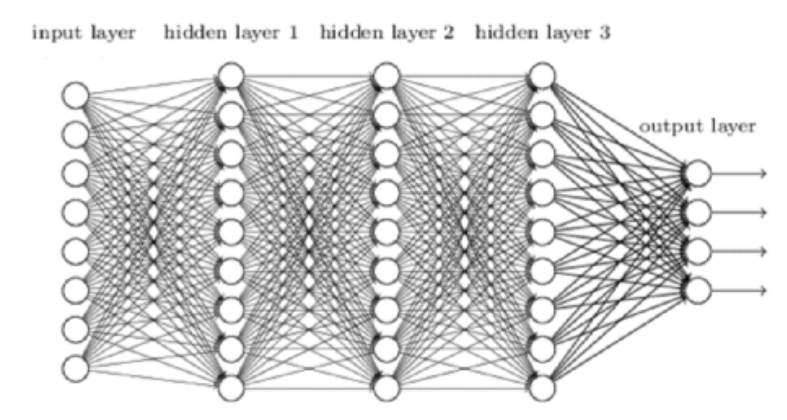
\includegraphics[width=\textwidth, scale=0.3]{Images/ann_2}

\caption[\textgreek{Νευρωνικό Δίκτυο}]{\textgreek{\textbf{Τεχνητό Νευρωνικό Δίκτυο}. Η είσοδος αποτελείται από κόμβους οι οποίοι δέχονται ένα γεγονός. Η επεξεργασία γίνεται εσωτερικά στους εσωτερικούς κόμβους. Ο αριθμός των επιπέδων ενός Δικτύου δεν είναι προκαθορισμένος και μπορεί να περάσει από πολλά επίπεδα μέχρι να πάρουμε στην έξοδο ένα επιθυμητό αποτέλεσμα.} \cite{brain_neuron}}
 \label{fig:ann}
\end{figure}

\section{\textgreek{Συνελικτικά Νευρωνικά Δίκτυα} (CNN)}
\textgreek{Μια κατηγορία Νευρωνικών Δικτύων είναι τα Συνελικτικά Νευρωνικά Δίκτυα, τα οποία έχουν εφαρμογές σε προβλήματα επεξεργασίας εικόνας και υπολογιστικής όρασης. Αποτελούνται από ένα ή περισσότερα επίπεδα συνέλιξης}
(convolutional layers) \textgreek{συχνά ακολουθούμενα από ένα επίπεδο υποδειγματοληψίας ακολουθούμενο από ένα ή περισσότερα πλήρως διασυνδεδεμένα επίπεδα όπως συναντάμε και σε ένα πολυεπίπεδο Νευρωνικό Δίκτυο. Η αρχιτεκτονική του ΣΝΔ σχεδιάζεται έτσι ώστε να εκμεταλλεύεται την δισδιάστατη δομή των εικόνων εισόδου ή άλλα δισδιάστατα σήματα όπως σήματα ήχου (π.χ. Φασματόγραμμα). Αυτό επιτυγχάνεται με τοπικές συνδέσεις και κατάλληλα βάρη προκειμένου να δημιουργηθούν χαρακτηριστικά ανεξαρτήτως μετατοπίσεων } (translation-invariant). \textgreek{Άλλο ένα πλεονέκτημα των ΣΝΔ είναι ότι είναι ευκολότερα στην εκπαίδευση και έχουν πολύ λιγότερες παραμέτρους από τα ΝΔ που έχουν πλήρως συνδεδεμένα επίπεδα.

\par 
Η είσοδος σε ένα επίπεδο συνέλιξης είναι μια $m\times n\times c$ εικόνα όπου $m$ και $n$ είναι το ύψος και το πλάτος της εικόνας αντίστοιχα, ενώ το $c$ είναι ο αριθμός των καναλιών, για παράδειγμα για έγχρωμες εικόνες }RGB $c = 3$. \textgreek{Το επίπεδο συνέλιξης έχει $k$ φίλτρα} (kernels) \textgreek{μεγέθους $w\times w \times r $ όπου είναι μικρότερο από τη διάσταση της εικόνας και μπορεί να είναι ίδιου μεγέθους με τα κανάλια ή μικρότερου και μπορεί να ποικίλει για κάθε φίλτρο. Το μέγεθος των φίλτρων προκαλεί τοπικά συνδεδεμένη δομή όπου το καθένα συνελίσσεται με κάθε εικόνα για να παράγουν χάρτες χαρακτηριστικών} (feature maps) \textgreek{μεγέθους $(m-w+1)\times (n-w+1)$. Κάθε χαρακτηριστικό υποδειγματοληπτείται τυπικά με κάποιο} pooling \textgreek{επίπεδο σε $p\times p$ συνεχείς περιοχές όπου το $p$ παίρνει συνήθως τιμές μεταξύ 2 και 5 αλλά για μεγάλες εικόνες εισόδου συναντάμε και μεγαλύτερα. Πριν ή μετά το }pooling layer \textgreek{συνήθως ακολουθεί μια προσθήκη μίας παραμέτρου πόλωσης }(bias) \textgreek{και μια συνάρτηση ενεργοποίησης σε κάθε χάρτη χαρακτηριστικών. Η εικόνα }\ref{fig:conv_layer} \textgreek{μας δείχνει ένα παράδειγμα ενός επιπέδου συνέλιξης.}

\begin{figure}[H]
 \centering
 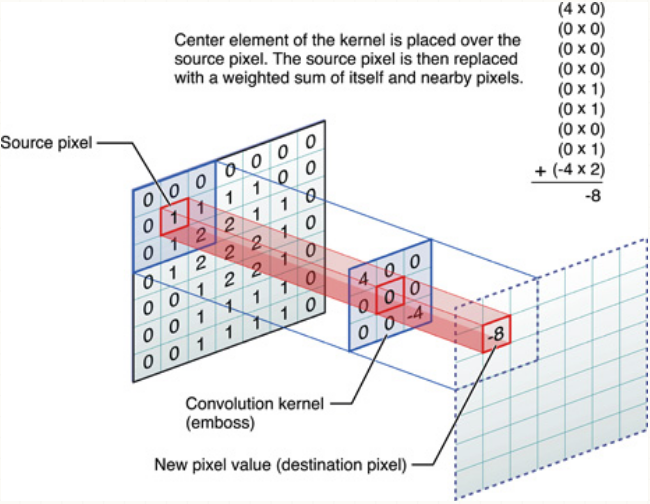
\includegraphics[width=\textwidth, scale=0.5]{Images/cnn_layer}
\caption[\textgreek{Επίπεδο Συνέλιξης}]{\textgreek{Επίδειξη ενός βήματος εφαρμογής ενός μικρού μεγέθους φίλτρου ($3\times 3$) σε έναν χάρτη χαρακτηριστικών εισόδου και το αποτέλεσμά της} \cite{cnnprimer}.}
 \label{fig:conv_layer}
\end{figure}
%%% LENET
\textgreek{Στην εικόνα }\ref{fig:lenet} \textgreek{βλέπουμε την πρώτη αρχιτεκτονική} CNN \textgreek{από τον }Yann LeCun \textgreek{για εφαρμογή σε προβλήματα αναγνώρισης ψηφίων. }

\begin{figure}[H]
 \centering
 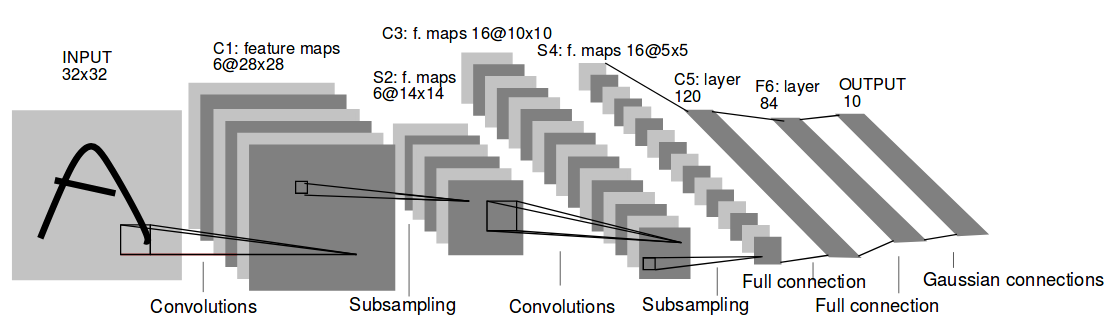
\includegraphics[width=\textwidth, scale=0.5]{Images/lenet_5}
\caption[\textgreek{ΣΝΔ }Lenet-5]{\textbf{CNN LeNet-5}.\textgreek{Αρχιτεκτονική του πρώτου Συνελικτικού Νευρωνικού Δικτύου για αναγνώριση ψηφίων από εικόνες. Κάθε επίπεδο αποτελεί ένα χαρτογράφημα των χαρακτηριστικών} \cite{lecun_net}.}
 \label{fig:lenet}
\end{figure}

\textgreek{Το } Alex-Net \textgreek{(εικόνα \ref{fig:alexnet_img}) ήταν μια δημιουργία των }Alex Krizhevsky, Ilya Sutskever, \textgreek{και} Geoffrey Hinton, \textgreek{και σηματοδότησε μια νέα εποχή στην υπολογιστική όραση καθώς πλέον περάσαμε στα \emph{Βαθιά} ΝΔ. Το εφάρμοσαν σε ένα από τα πιο απαιτητικά προβλήματα, το} \href{http://www.image-net.org/}{\emph{Image-Net}} \cite{imagenet_bib}. \textgreek{Η συγκεκριμένη αρχιτεκτονική κατάφερε να πετύχει ένα σημαντικό αποτέλεσμα μειώνοντας πάνω από 10\% το σφάλμα σε σχέση με τον προηγούμενο νικητή το 2012, πάνω σε ένα πρόβλημα με 15 εκατομμύρια εικόνες και 1000 κατηγορίες για αναγνώριση. Σε αυτό το μοντέλο ήταν και η πρώτη εφαρμογή των γραμμικών ανορθωτών ως συνάρτηση ενεργοποίησης αλλά και η χρήση συνθετικών δεδομένων. Αυτή η συνεισφορά είναι τόσο σημαντική καθώς οι περισσότερες τεχνικές χρησιμοποιούνται μέχρι και σήμερα.}

%% ALEXNET
\begin{figure}[H]
 \centering
 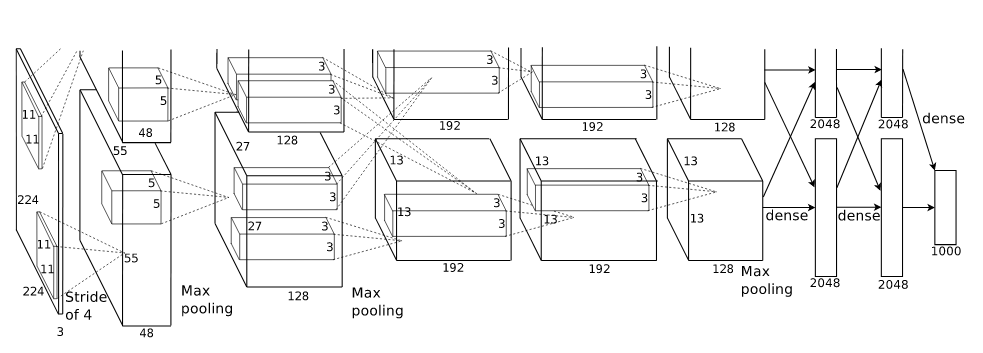
\includegraphics[width=\textwidth, scale=0.5]{Images/alex_net}
\caption[\textgreek{ΣΝΔ }Alex-Net]{\textbf{Alex-Net}.\textgreek{Αρχιτεκτονική του }Alex-Net \textgreek{ένα από τα πρώτα Βαθιά ΝΔ με 60 εκατομμύρια παραμέτρους και 650.000 νευρώνες.} \cite{alex_net_bib}.}
 \label{fig:alexnet_img}
\end{figure}

\section{\textgreek{Πλήρως Συνελικτικά Νευρωνικά Δίκτυα}}
\textgreek{Μία ακόμα κατηγορία ΝΔ με τα οποία θα ασχοληθούμε στο υπόλοιπο της εργασίας είναι τα Πλήρως ΣΝΔ} (Fully-CNN) \cite{fcnn_1}. \textgreek{Η κύρια διαφορά με τα ΣΝΔ είναι η απώλεια πλήρως συνδεδεμένων επιπέδων στην έξοδο }(fully-connected layers), \textgreek{εν αντιθέσει με τα ΣΝΔ που είδαμε προηγουμένως, δηλαδή τα ΠΣΝΔ μαθαίνουν πληροφορία μόνο από φίλτρα. Τα ΠΣΝΔ θεωρούνται κατάλληλα για προβλήματα Σημασιολογικής Κατάτμησης αντικειμένων από εικόνες (εικόνα} \ref{fig:fcn_img}).

%FCN_1
\begin{figure}[H]
 \centering
 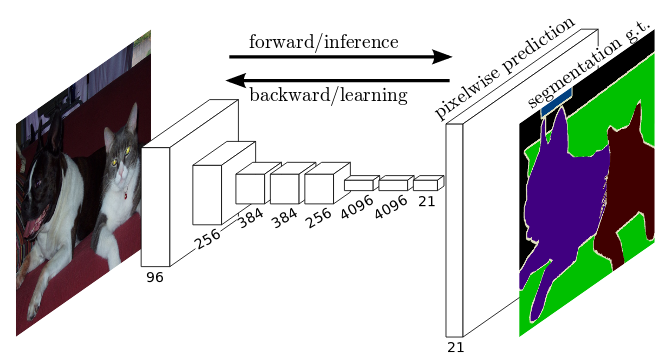
\includegraphics[width=\textwidth, scale=0.5]{Images/fcn_1}
\caption[Fully-CNN]{\textgreek{Πλήρως ΣΝΔ} (Fully CNN) \textgreek{μπορούν να μάθουν αποδοτικά να κάνουν προβλέψεις σε προβλήματα αναγνώρισης σε επίπεδο εικονοστοιχείων} \cite{fcnn_1}.}
 \label{fig:fcn_img}
\end{figure}



\textgreek{Μερικά θετικά στοιχεία που καταστούν τα ΠΣΝΔ κατάλληλα για Σημασιολογική Κατάτμηση είναι σε αντίθεση με άλλου είδους ΝΔ είναι}:

\begin{description}[labelindent=10pt, style=multiline, leftmargin=30pt]
 \item[1.] \textgreek{Χρησιμοποιούν όλη την πληροφορία της εικόνας.}
 \item[2.] \textgreek{Κρατάνε την χωρική πληροφορία} (spatial information) \textgreek{από την εικόνα.}
 \item[3.] \textgreek{Είναι πιο γρήγορα στην εκπαίδευση αλλά και στην συμπερασματολογία.}
 \item[4.] \textgreek{Είναι αμετάβλητα ως προς το μέγεθος εισόδου της εικόνας.}
\end{description}
\pagebreak
\section{\textgreek{Εμπρόσθια Διάδοση}}
\textgreek{Η Εμπρόσθια Διάδοση }(Forward Propagation) \textgreek{είναι ο τρόπος με τον οποίο το ΣΝΔ επεξεργάζεται τα δεδομένα. Τα ΣΝΔ έχουν δημιουργηθεί με την προοπτική να επεξεργάζονται δεδομένα από εικόνες. Αποτελούνται από πολλά επίπεδα συνέλιξης τα οποία είναι συνδεδεμένα σειριακά για να επεξεργάζονται οπτική πληροφορία. Τα συνελικτικά επίπεδα αποτελούνται από μια σειρά από φίλτρα $\mathbf{\mathit{K}}$ και τις πολώσεις $\mathbf{\mathit{b}}$} (biases), \textgreek{ ενώ δέχονται έναν χάρτη χαρακτηριστικών στην είσοδο $\mathbf{\mathit{I}}$.}
\par
\textgreek{Στην περίπτωση που έχουμε εικόνες για αναγνώριση, η είσοδος αποτελείται από μια εικόνα με ύψος $\mathbf{\mathit{H}}$, πλάτος $\mathbf{\mathit{W}}$  και αριθμό καναλιών $\mathbf{\mathit{C =3 }}$ (κόκκινο, πράσινο και μπλε), $\mathbf{\mathit{I \in \mathbb{R}^{H\times W\times C}}}$. Επομένως, για μια σειρά από $D$ φίλτρα έχουμε $K \in \mathbb{R}^{k_1\times k_2\times C\times D}$ και $b \in \mathbb{R}^{D}$ πολώσεις, μία για κάθε φίλτρο. Για κάθε στοιχείο $i,j$ του χάρτη χαρακτηριστικών εισόδου $I$ εφαρμόζουμε την συνέλιξη με τον πυρήνα $K$:}

\begin{equation}
(I \ast K)_{ij} = \sum_{m=0}^{k_1-1} \sum_{n=0}^{k_2-1} \mathit{K_{m,n,c}} \cdot \mathit{I_{i+m,j+n,c}} + \mathit{b}
\end{equation}

\textgreek{Πιο αναλυτικά, η παραπάνω εξίσωση αναλύεται για κάθε επίπεδο συνέλιξης με τις εξής παραμέτρους:}

\begin{enumerate}
 \item l : \textgreek{Συμβολίζει το επίπεδο συνέλιξης $l$ όπου $l = 1$ είναι το πρώτο επίπεδο και $l = L$ το τελευταίο επίπεδο.}
\item \textgreek{$x$ είναι η είσοδος με διαστάσεις $H\times W$ και με $i,j$ συμβολίζουμε τους δείκτες του πολυδιάστατου διανύσματος.}
\item \textgreek{Φίλτρο $w$ διαστάσεων $k_1\times k_2$ όπου έχει ως δείκτες τα $m,n$.}
\item \textgreek{$w_{m,n}^{l}$ είναι ο πίνακας με τα βάρη που συνδέει του νευρώνες του επιπέδου $l$ με τους νευρώνες του επιπέδου $l-1$.}
\item \textgreek{$x_{i,j}^{l}$ είναι το διάνυσμα εισόδου του επιπέδου $l$}:\\[1em]
\centerline{ $x_{i,j}^{l} = \sum_{m} \sum_{n} w_{m,n}^{l} o_{i+m,j+n}^{l-1} + b^{l}$}

\item \textgreek{$b^{l}$ είναι το διάνυσμα πόλωσης.}
\item \textgreek{$o_{i,j}^{l}$ είναι το διάνυσμα εξόδου στο επίπεδο $l$}:\\[1em]
\centerline{$ o_{i,j}^{l} = f(x_{i,j}^{l})$}
\item \textgreek{ $f(\cdot)$ είναι η συνάρτηση ενεργοποίησης, η οποία εφαρμόζεται στην είσοδο μετά την διαδικασία της συνέλιξης στο επίπεδο $l$.}
\end{enumerate}

\pagebreak
\section{\textgreek{Αλγόριθμος Οπισθοδρόμησης}}
\textgreek{Ο αλγόριθμος οπισθοδρόμησης }(backpropagation) \cite{bptt_1} \textgreek{αποτελεί την μέθοδο με την οποία ένα ΝΔ επαναπροσδιορίζει τις παραμέτρους του. Αποτελεί έναν από τους πιο βασικούς αλγορίθμους για την εκπαίδευση των ΝΔ σε προβλήματα επιβλεπόμενης μάθησης }(supervised learning). \textgreek{Η συνάρτηση κόστους που χρησιμοποιούμε σε αυτό το πρόβλημα όπως θα αναλύσουμε παρακάτω (παράγραφος }\ref{sec:loss_function})\textgreek{ είναι η συνάρτηση διεντροπίας και είναι παραγωγίσιμη και έχει πολύ απλή παράγωγο.}
\par
\textgreek{Ο αλγόριθμος οπισθοδρόμησης χρησιμοποιείται για τον υπολογισμό των παραγώγων σφάλματος. Ο αλγόριθμος αποτελείται από την εφαρμογή του κανόνα της αλυσίδας για τον υπολογισμό των μερικών παραγώγων. Αρχικά, υπολογίζουμε την μερική παράγωγο της συνάρτησης κόστους ως προς την μεταβλητή εξόδου και την μερική παράγωγο της εξόδου από την } softmax ($y_i$) \textgreek{ως προς την μεταβλητή της εισόδου της μονάδας }softmax ($s_i$). \textgreek{Επομένως, χρησιμοποιώντας τον κανόνα της αλυσίδας για να υπολογίσουμε τις παραγώγους της συνάρτησης κόστους ως προς την είσοδο της μονάδας }softmax. \textgreek{Στις εξισώσεις παρακάτω, $y_i$ είναι η έξοδος του $i$ στοιχείου ενώ $s_i$ είναι η η είσοδος του $i$ στοιχείου }\cite{backprop_notes}.  

\begin{equation}
 \frac{\partial E}{\partial y_i} = -\frac{t_i}{y_i}
\end{equation}

\begin{equation}
 \frac{\partial y_i}{\partial s_i} = y_i(1-y_i)
\end{equation}

\begin{equation}
 \frac{\partial E}{\partial s_i} =\frac{\partial E}{\partial y_i} \frac{\partial y_i}{\partial s_i} = y_i-t_i
\end{equation}
\textgreek{Εφαρμόζοντας τον κανόνα της αλυσίδας, προχωράμε προς τα κρυφά επίπεδα }(hidden layers) \textgreek{προς τα πίσω. Για να διαδώσουμε τις παραγώγους του $i$ στοιχείου στο $j$ στοιχείο το οποίο ανήκει στο προηγούμενο επίπεδο, προκύπτουν οι παρακάτω εξισώσεις} (\ref{eqn:back_4} \textgreek{και} \ref{eqn:back_5}) \textgreek{όπου $w_{ji}$ είναι το βάρος που ανατίθεται στην σύνδεση μεταξύ της εισόδου του $j$ στοιχείου με την κρυφή μονάδα $i$. Εφαρμόζοντας επαναληπτικά τον κανόνα της αλυσίδας διαδίδουμε τις παραγώγους του σφάλματος προς την είσοδο του ΝΔ. Με αυτήν την μέθοδο έχουμε καταφέρει να υπολογίσουμε τις παραγώγους σφάλματος για κάθε βάρος.}

\begin{equation}
\label{eqn:back_4}
 \frac{\partial E}{\partial y_i} =\frac{\partial E}{\partial s_i} \frac{\partial s_i}{\partial y_j}=\sum_i w_{ji} \frac{\partial E}{\partial s_i} 
\end{equation}

\begin{equation}
\label{eqn:back_5}
\frac{\partial E}{\partial w_{ji}} =\frac{\partial E}{\partial s_i} \frac{\partial s_i}{\partial w_{ji}} = (y_i-t_i)\frac{\partial s_i}{\partial w_{ji}}
\end{equation}

\textgreek{Στα επίπεδα συγκέντρωσης διαφέρει η διαδικασία της οπισθοδρόμησης ανάλογα με το είδος του επιπέδου συγκέντρωσης. Ένα επίπεδο συγκέντρωσης δεν περιέχει παραμέτρους μάθησης} \cite{pooling}.\textgreek{ Τα πιο δημοφιλή επίπεδα συγκέντρωσης είναι τα επίπεδα μέγιστης και μέσης συγκέντρωσης αντίστοιχα. Στο επίπεδο συγκέντρωσης, η εμπρόσθια διάδοση έχει ως αποτέλεσμα στην έξοδο έναν μειωμένο χάρτη χαρακτηριστικών όπου έχει εφαρμοστεί ένα $N\times N$ τμήμα συγκέντρωσης σε κάθε περιοχή και στην έξοδο εξέρχεται μόνο ένα στοιχείο από το τμήμα. Η Οπισθοδρόμηση στο επίπεδο συγκέντρωσης, οπισθοδρομεί το σφάλμα το οποίο έχει προέλθει από την μοναδική επικρατέστερη τιμή του κάθε τμήματος. 
\par 
Για να κρατήσουμε την θέση της επικρατέστερης τιμής από το επίπεδο συγκέντρωσης, σημειώνουμε την θέση κατά την εμπρόσθια διάδοση και μετά την χρησιμοποιούμε για να οδηγήσουμε τις παραγώγους του σφάλματος κατά την οπισθοδρόμηση. Η δρομολόγηση των παραγώγων επιτυγχάνεται με κάποια από τις παρακάτω μεθόδους, ανάλογα το επίπεδο συγκέντρωσης}:
\par 
% 
\begin{description}[labelindent=1.7cm, style=unboxed, leftmargin=2.1cm, font=$\bullet$~]
  \item[Max-Pooling] \textgreek{Το σφάλμα απλώς ανατίθεται στο στοιχείο το οποίο επικράτησε κατά το εμπρόσθιο πέρασμα. }
  \item[Average-Pooling] \textgreek{Το σφάλμα πολλαπλασιάζεται με τον παράγοντα $\frac{1}{N\times N}$ και η προκύπτουσα τιμή ανατίθεται σε ολόκληρο το τμήμα συγκέντρωσης, δηλαδή όλα τα στοιχεία παίρνουν την ίδια κανονικοποιημένη τιμή.} 
\end{description}



\chapter{\textgreek{Μεθοδολογία}}
\label{chapter_2}

\pagestyle{fancy}
\fancyhf{}
%\fancyhead[OC]{\leftmark \textgreek{Τι φάση}}
%\fancyhead[C]{}
%\fancyhead[EC]{\rightmark}
\renewcommand{\footrulewidth}{0.5pt}
\cfoot{\thepage}

\section{\textgreek{Εισαγωγή}}
\textgreek{Στο κεφάλαιο αυτό θα συζητήσουμε για τις μεθόδους και τις τεχνικές που χρησιμοποιήθηκαν στην εργασία μας αλλά και την ανάλυση με λεπτομέρειες των αλγορίθμων που εφαρμόστηκαν. Συγκεκριμένα, θα δούμε τις αρχιτεκτονικές βαθειάς μάθησης που χρησιμοποιήσαμε στα πειράματα, καθώς και την θεωρία αυτών. Η μεθοδολογία μας βασίστηκε στους αλγορίθμους των Νευρωνικών Δικτύων και πιο συγκεκριμένα στα Πλήρως Συνελικτικά Νευρωνικά Δίκτυα} FCNN \textgreek{που έχουν εφαρμογές σε προβλήματα της όρασης υπολογιστών και πιο συγκεκριμένα στην Σημασιολογική Κατάτμηση πληροφορίες από εικόνες. Η προσέγγιση μας περιλαμβάνει δύο μοντέλα τα οποία αποτελούνται από τρία στάδια: Κωδικοποίηση Χαρακτηριστικών, Παράλληλη Επεξεργασία και Αποκωδικοποίηση} (Encoder-Parallel Processing-Decoder). 

\section{\textgreek{Πρώτη Προσέγγιση}} 
\textgreek{Η πρώτη μας προσέγγιση στο πρόβλημα βασίστηκε σε μια παράλληλη αρχιτεκτονική από πολλαπλά ΣΝΔ (εικόνα} \ref{fig:cnn_1}). \textgreek{Η ιδέα στηρίχθηκε στην υλοποίηση τεσσάρων ΣΝΔ όπου τα 3 από αυτά δέχονται σαν είσοδο σειριακά κομμάτια από την εικόνα. Η μέθοδος αυτή αναφέρεται ως \emph{``Ολίσθηση Παραθύρων``}} \emph{(Sliding-Windows)} \cite{sliding_window}. \textgreek{Τα τρία από τα τέσσερα ΣΝΔ δέχονται κομμάτια διαφορετικού μεγέθους από την εικόνα, ενώ το τέταρτο ΣΝΔ δέχεται σαν είσοδο ολόκληρη την εικόνα. Έτσι παίρνουμε 4 διαφορετικές προβλέψεις για κάθε εικονοστοιχείο και αποφασίζουμε κατά πλειψηφία το επικρατέστερο.}\par

\textgreek{Η ιδέα αυτή αν και πολύ απλή είχε αρκετές δυσκολίες}:

\begin{description}[labelindent=10pt, style=multiline, leftmargin=30pt]
 \item[1.] \textgreek{Τα μικρά κομμάτια τμηματοποιούν κάποια αντικείμενα κατά την εκπαίδευση και καθίσταται δύσκολη η αναγνώριση τους καθώς δεν μαθαίνουν κάποια ολοκληρωμένη δομή από αυτά.}
 \item[2.] \textgreek{Η διαδικασία της δοκιμής ήταν σχεδόν ανέφικτη καθώς ένα τέτοιο μοντέλο είναι πολύ δαπανηρό σε πόρους.}
 \item[3.] \textgreek{Η μέθοδος Ολίσθησης Παραθύρων είναι πολύ αργή.}
\end{description}

\par \textgreek{Σύμφωνα με τα παραπάνω, δεν θα ασχοληθούμε περαιτέρω με αυτή την αρχιτεκτονική, αλλά προχωρήσαμε σε διαφορετική προσέγγιση του προβλήματος όπως θα δούμε στην συνέχεια.}

\begin{figure}[H]
 \centering
 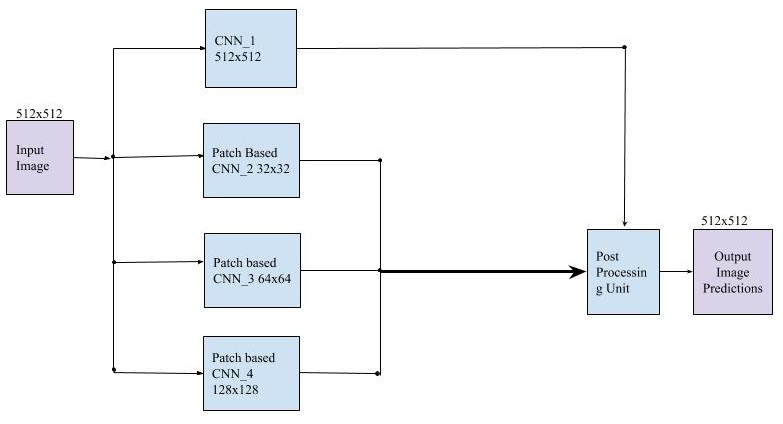
\includegraphics[scale=0.5]{Images/patch_cnn}
 \caption[\textgreek{Παράλληλο ΣΝΔ}]{\textgreek{Παράλληλη αρχιτεκτονική βασισμένη σε πολλαπλά ΣΝΔ με διαφορετικά μεγέθη ειδόδου το καθένα. }}
  \label{fig:cnn_1}
\end{figure}


\section{\textgreek{Προετοιμασία Δεδομένων}}
\textgreek{Η προετοιμασία των δεδομένων μας αποτελεί το πρώτο στάδιο, το οποίο κρίνεται αναγκαίο ώστε να γίνει εφικτή η εφαρμογή των αλγορίθμων βαθειάς μάθησης καθώς χωρίς αυτό το στάδιο δεν θα μπορέσουμε να έχουμε τα επιθυμητά αποτελέσματα.} 

\subsection{\textgreek{Υποδειγματοληψία}}
\label{sec:bilinear}
\textgreek{Η βάση δεδομένων μας αποτελείται από εικόνες υψηλής ευκρίνειας. Τα νευρωνικά δίκτυα έχουν πολλά εκατομμύρια παραμέτρους, οι παράμετροι είναι συνάρτηση της εισόδου του νευρωνικού δικτύου, επομένως η υποδειγματοληψία στις αρχικές εικόνες είναι απαραίτητη για να μπορέσουμε να κάνουμε εφικτά τα πειράματά μας. Αυτή η τεχνική φυσικά έχει κάποιο κόστος, καθώς η μείωση των διαστάσεων των εικόνων σημαίνει απώλεια σε πληροφορία. 


Για την υποδειγματοληψία στις εικόνες χρησιμοποιήθηκαν δύο διαφορετικοί αλγόριθμοι. Ο πρώτος είναι ο αλγόριθμος της Διγραμμικής Παρεμβολής} (Bilinear Interpolation) \textgreek{και ο δεύτερος είναι αυτός των Πλησιέστερων Γειτόνων.

\par 
Τον αλγόριθμο της Διγραμμικής Παρεμβολής τον χρησιμοποιήσαμε για την υποδειγματοληψία της εικόνας καθώς το εικονοστοιχείο που δημιουργείται κατά την διαδικασία της υποδειγματοληψίας προσεγγίζεται από μια σταθμισμένη εκτίμηση από άλλα τέσσερα σημεία ως μια καλύτερη προσέγγιση των εικονοστοιχείων.}


\textgreek{Ο αλγόριθμος του Πλησιέστερου Γείτονα, γνωστός και ως αλγόριθμος Παρεμβολής μηδενικής τάξης εφαρμόστηκε στις εικόνες με τις ετικέτες των εικονοστοιχείων} (ground truth). \textgreek{Ο λόγος που χρησιμοποιήσαμε αυτήν την απλή προσέγγιση είναι η εξασφάλιση των επιθυμητών ετικετών κατά τη διάρκεια της δειγματοληψίας. Συγκεκριμένα, το καινούριο εικονοστοχείο προέρχεται από το πλησιέστερο ως προς το μέγεθος εικονοστοιχείο, επομένως κάποιος άλλος αλγόριθμος θα μας παραποιούσε τις ετικέτες των εικονοστοιχείων. }

% \begin{figure}[h]
% %  \centering
% %  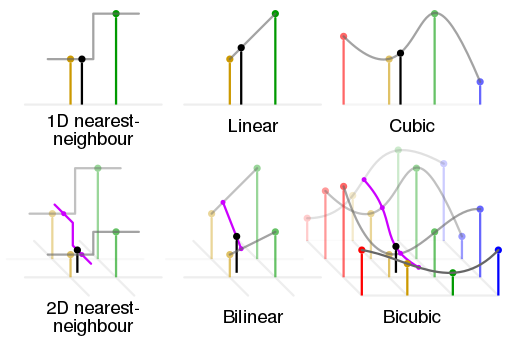
\includegraphics[scale=0.7]{Images/all_inter}
% %  \caption[\textgreek{Μέθοδοι Παρεμβολής}]{\textgreek{Μέθοδοι Παρεμβολής} \cite{wiki_interpolation}.}
%  \label{fig:all_inter_img}
% \end{figure}

\subsection{\textgreek{Κανονικοποίηση Χαρακτηριστικών}}
\textgreek{Η  κανονικοποίηση των χαρακτηριστικών }(feature normalization),\textgreek{ εφαρμόζεται στα χαρακτηριστικά των δεδομένων, στην δική μας περίπτωση τις εικόνες και έχει ως αποτέλεσμα να φέρει τα δεδομένα στην ίδια κλίμακα με μικρές διακυμάνσεις μεταξύ τους. Ο χώρος των χρωμάτων των εικόνων έχει μεγάλο εύρος $[0,255]$. Αυτό δημιουργεί πρόβλημα στην εκπαίδευση των ΝΔ καθώς μπορεί να πάρουν ανεξέλεγκτες τιμές οι νευρώνες στα }hidden layers \textgreek{και να μην συγκλίνει το ΣNΔ Ο λόγος που βελτιώνει την σύγκλιση είναι επειδή οι τιμές στην είσοδο έχουν μέση τιμή μηδέν και διασπορά ένα, ως αποτέλεσμα οι νευρώνες στα ενδιάμεσα επίπεδα δεν μπαίνουν σε κορεσμό τόσο εύκολα και τόσο γρήγορα. Η εξίσωση }\ref{eqn:eq_feat_norm} \textgreek{μας εξασφαλίζει τα χαρακτηριστικά να βρίσκονται στον χώρο $[-1,1]$, έχοντας μέση τιμή μηδέν και διασπορά κοντά στο ένα. Για τον υπολογισμό της μέσης τιμής του συνόλου δεδομένων χρησιμοποιήσαμε ένα δείγμα από αυτό, από 500 δείγματα} \cite{feat_norm}.


\begin{equation}
 \hat{\mu} = \frac{\sum_{i=1}^{N} X_{i}}{N} 
 \label{mean}
\end{equation}
\\[1cm]

\begin{equation}
 X = \frac{X - \hat{\mu}}{max(X) - min(X)}
 \label{eqn:eq_feat_norm}
\end{equation}

\subsection{\textgreek{Δυσαναλογία των Κλάσεων}}
\textgreek{Ένα πολύ συχνό πρόβλημα που υπάρχει στα περισσότερα σύνολα δεδομένων, είναι η δυσαναλογία των κλάσεων ή κατηγοριών. Η δυσαναλογία προκύπτει όταν σε ένα σύνολο δεδομένων υπάρχουν μεγάλες διαφορές μεταξύ του πλήθους των στοιχείων που ανήκουν σε ορισμένες κατηγορίες. Το πρόβλημα αυτό δεν το λύνουν τα νευρωνικά δίκτυα από μόνα τους, καθώς τείνουν να μάθουν καλύτερα πληροφορίες για τα στοιχεία που αποτελούν πλειοψηφία στο σύνολο δεδομένων μας, ενώ τα στοιχεία που αποτελούν μειονότητα φτάνουν σε σημείο μέχρι και να αγνοούνται. Μία λύση σε αυτό το πρόβλημα θα μπορούσε να είναι η υπερδειγματοληψία των κλάσεων που είναι μειονότητα, έτσι ώστε να δημιουργήσουμε ισόποσα σύνολα κλάσεων για να υπάρξει ισοστάθμιση. Όμως αυτή η τεχνική είναι ανέφικτη σε ένα σύνολο από εικόνες όπου θα πρέπει να δημιουργήσουμε καινούρια εικονοστοιχεία που να ανήκουν σε κάποια συγκεκριμένη κατηγορία. 

\par Για την λύση αυτού του προβλήματος εφαρμόστηκε η Συνάρτηση Μέσης Συχνότητας Ισορροπίας }(Median Frequency Balance) \cite{median_freq}. \textgreek{Με αυτή την συνάρτηση βρίσκουμε τους συντελεστές και τους εφαρμόζουμε στην συνάρτηση κόστους (εξίσωση} \ref{eqn:loss_func}). \textgreek{\par Η ιδέα είναι να βρεθούν οι συντελεστές συχνότητας οι οποίοι προέρχονται από την συχνότητα εμφάνισης ενός εικονοστοιχείου που ανήκει σε μια κατηγορία. Όταν ένα εικονοστοιχείο $i$ ανήκει στην κατηγορία $j$ (όπου είναι μειονότητα) και βρίσκεται κατά την διαδικασία της μάθησης να είναι στην κατηγορία $k$ τότε επιβάλλεται μεγαλύτερη ποινή και διαδίδεται μεγαλύτερο σφάλμα προς τα πίσω. Αυτό συμβαίνει επειδή το νευρωνικό δίκτυο δεν θα δει πολλές φορές μια κλάση που είναι μειονότητα οφείλουμε να εισάγουμε μεγαλύτερη ποινή για να βοηθήσουμε στην εκμάθηση τους. 

\par Με την εξίσωση }\ref{eqn:ratio} \textgreek{βρίσκουμε την συχνότητα εμφάνισης των εικονοστοιχείων για κάθε κλάση στο σύνολο δεδομένων και αφού ταξινομήσουμε τις τιμές συχνότητας παίρνουμε την μεσαία συχνότητα και την χρησιμοποιούμε σαν επίκεντρο} \textgreek{τοποθετώντας την στον αριθμητή (εξίσωση }\ref{eqn:alpha_coef}). \textgreek{Με αυτή την μέθοδο πετυχαίνουμε να έχουμε υψηλούς συντελεστές $a_i$ στα χαμηλής συχνότητας εμφάνισης εικονοστοιχεία. Με την εξίσωση} \ref{eqn:alpha_coef} \textgreek{βρίσκουμε τους συντελεστές $a$ για κάθε κατηγορία αντικειμένων. Ένας μεγάλος συντελεστής $a_i$ προσθέτει μεγαλύτερη ποινή όταν ταξινομηθεί λάθος ένα εικονοστοιχείο που ανήκει σε μια κλάση που δεν υπάρχει πολλές φορές στο σύνολο δεδομένων. Τέλος, στα δεδομένα μας, υπάρχουν εικονοστοιχεία τα οποία δεν ανήκουν σε κάποια κατηγορία, για να μην μάθει το ΝΔ από αυτά θέσαμε τον συντελεστή $a_i$ στο μηδέν έτσι ώστε να μην συνεισφέρουν στο σφάλμα κατά την εκπαίδευση.} 

\noindent\begin{minipage}{.5\linewidth}
  \begin{equation}
    freq(C_{i}) = \frac{C_{i}}{\sum_{i=1}^{Classes} C_{i}}
    \label{eqn:ratio}
  \end{equation}
\end{minipage}%
\begin{minipage}{.5\linewidth}
  \begin{equation}
  \alpha_{i} = \frac{median(freq)}{freq(C_{i})}
  \label{eqn:alpha_coef}
  \end{equation}
\end{minipage}


\subsection{\textgreek{Επισκόπηση Αρχιτεκτονικής}}

\subsubsection{\textgreek{Αρχικοποίηση Παραμέτρων Πυρήνα}}
\textgreek{Η αρχικοποίηση των παραμέτρων των φίλτρων αποτελεί ένα σημαντικό στάδιο στην εκπαίδευση των Νευρωνικών Δικτύων. Στόχος της αρχικοποίησης είναι η μέση τιμή της εισόδου και εξόδου ενός επιπέδου να είναι κοντά στο μηδέν αλλά και η διασπορά τους να είναι κοντά στο ένα, καθώς αποτρέπει τους Νευρώνες να μπουν σε κορεσμό. Τα βάρη του ΣΝΔ δειγματοληπτήθηκαν από μία Γκαουσιανή κατανομή με μέση τιμή ίση με το μηδέν ($\mu=0$) και διασπορά ίση με ένα ($\sigma^2 = 1/N$). Η εξίσωση} \ref{eqn:lecun_norm} \textgreek{μας δείχνει την τυπική απόκλιση που εφαρμόστηκε στην κατανομή Γκάους (εξίσωση} \ref{eqn:gauss}) \textgreek{για την δειγματοληψία των βαρών όπου με $N$ συμβολίζεται το πλήθος των χαρακτηριστικών της εισόδου σε κάθε επίπεδο συνέλιξης. } 

\begin{equation}
 \label{eqn:lecun_norm}
  \centering
 \mathit{\sigma} = \sqrt{\frac{1}{\textit{N}}}
\end{equation}

\begin{equation}
 \label{eqn:gauss}
  \centering
 g(x) = \frac{1}{\sigma \sqrt{2\pi}} e^{\frac{1}{2}(\frac{x-\mu}{\sigma})^{2}}
\end{equation}

\subsubsection{\textgreek{Συνάρτηση Ενεργοποίησης}}
\textgreek{Άλλη μια απαραίτητη συνάρτηση για τα Νευρωνικά Δίκτυα είναι η συνάρτηση ενεργοποίησης. Εφαρμόζεται στην έξοδο των επιπέδων των νευρωνικών δικτύων και είναι υπεύθυνη για την ανταλλαγή μηνυμάτων μεταξύ νευρώνων στα επίπεδα από νευρώνες. Τα βαθειά νευρωνικά δίκτυα έρχονται αντιμέτωπα με το πρόβλημα της εξαφάνισης των αποκλίσεων του σφάλματος κατά την διάδοσή τους προς τα πίσω. Για τον λόγο αυτό επινοήθηκαν συναρτήσεις που ονομάζονται Γραμμικοί Ανορθωτές }(Linear Rectifiers). \textgreek{Οι γραμμικοί ανορθωτές συνήθως κάτω από το μηδέν έχουν μηδενική τιμή. Όταν οι αποκλίσεις πέφτουν κάτω από το μηδέν τα βάρη δεν αλλάζουν, δηλαδή οι νευρώνες μένουν απενεργοποιημένοι σε μια τέτοια περίπτωση. Το θετικό σε αυτήν την περίπτωση είναι ότι εφόσον κάποιοι νευρώνες τείνουν σε αδράνεια, το νευρωνικό γίνεται ελαφρύτερο από την άποψη των υπολογισμών. Από την άλλη, το μεγάλο μειονέκτημα είναι ότι αν βρεθούν σε αυτή την κατάσταση μπορεί να μην ξανά ενεργοποιηθούν οι νευρώνες και δεν θα ανταποκριθούν σε αλλαγές από μικρά σφάλματα. Αυτό ονομάζεται Φαινόμενο Νεκρών Νευρώνων. 
\par Μία λύση σε αυτό το πρόβλημα είναι η εισαγωγή μιας παραμετρικής συνάρτησης κάτω από το μηδέν, η οποία θα δίνει ένα μικρό ερέθισμα στους νευρώνες ώστε να αποφευχθεί αυτό το πρόβλημα. Για τον λόγο αυτό εισάγαμε στα νευρωνικά μας την Κλιμακωτή Εκθετική Γραμμική Συνάρτηση }(Scaled Exponential Linear Unit-SELU). \textgreek{Στην πραγματικότητα όπως απέδειξαν στο }\cite{self_norm}\textgreek{ η συγκεκριμένη συνάρτηση ενεργοποίησης σε συνδυασμό με την αρχικοποίηση (εξισώσεις }\ref{eqn:lecun_norm}, \ref{eqn:gauss}) \textgreek{όχι μόνο καταπολεμά αυτό το πρόβλημα αλλά καθιστά περιττή την εφαρμογή του αλγορίθμου }Batch-Normalization \cite{batch_norm} \textgreek{καθώς η κανονικοποίηση των εισόδων σε κάθε επίπεδο του νευρωνικού γίνεται μέσα σε αυτή την συνάρτηση, πετυχαίνοντας έτσι μείωση των παραμέτρων.}

\begin{figure}[H]
 \centering
 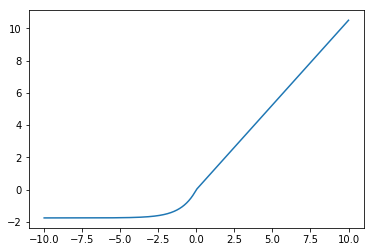
\includegraphics[scale=1.1]{Images/selu}
 \caption[SELU Function]{\textgreek{Κλιμακωτή Εκθετική Γραμμική Συνάρτηση Ενεργοποίησης} (SELU) \textgreek{με τις προεπιλεγμένες παραμέτρους $\alpha = 1.6732$\textgreek{ και} $\lambda = 1.0507$}.}
  \label{fig:selu_img}
\end{figure}


\begin{equation}
 f(x) = \lambda
\begin{cases}
    x   & \quad \text{if } x > 0 \\
    \alpha e^{x} - \alpha & \quad \text{if } x \leq 0
\end{cases}
\end{equation}


\begin{figure}[H]
 \label{act_func_img}
 \centering
 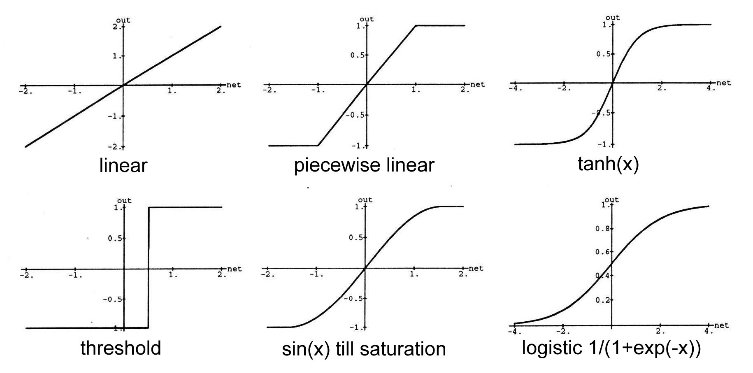
\includegraphics[scale=0.6]{Images/act_func}
 \caption[\textgreek{Συναρτήσεις Ενεργοποίησης}]{\textgreek{Διάφορες συναρτήσεις Ενεργοποίησης} \cite{act_funcs}}
\end{figure}


\subsubsection{\textgreek{Αλγόριθμοι Βελτιστοποίησης}}
\textgreek{Ο αλγόριθμος βελτιστοποίησης αποτελεί έναν πολύ σημαντικό παράγοντα για την εκπαίδευση ενός Νευρωνικού Δικτύου. Η ανάγκη για αναζήτηση αλγορίθμων βελτιστοποίησης προήλθε από δύο σημαντικούς παράγοντες. Πρώτον, λόγω των πολλών δεδομένων για επεξεργασία και των βαθιών νευρωνικών δικτύων που έκανε την διαδικασία της μάθησης αργή. Αυτοί οι λόγοι μας ώθησαν σε τεχνικές μείωσης του σφάλματος από κομμάτια του συνόλου δεδομένων και δεύτερων για την επιτάχυνση της σύγκλισης του Νευρωνικού δικτύου προφανώς.} 

\textgreek{Παρακάτω στην εικόνα }\ref{fig:sgd_regime} \textgreek{βλέπουμε πως αν η συνάρτηση κόστους έχει την μορφή μίας χαράδρας που οδηγεί προς το βέλτιστο κόστος και έχει στα πλάγια υψηλά τοιχώματα, τότε με ένα μεγάλο ρυθμό μάθησης τα βάρη τείνουν να ταλαντεύονται μπρος και πίσω επειδή η αρνητική απόκλιση τείνει προς τις απότομες πλευρές κάθε φορά αντί να πηγαίνει προς το βέλτιστο. Αυτό το φαινόμενο συμβαίνει σχεδόν πάντα και δημιουργεί πρόβλημα διότι μας κάνει την σύγκλιση πολύ αργή.}

\begin{figure}[H]
 \centering
 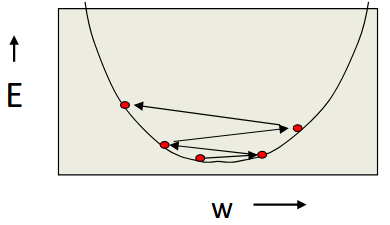
\includegraphics[scale=0.5]{Images/sgd_img}
 \caption[\textgreek{Ενέργεια Συνάρτησης Κόστους}]{\textgreek{Ταλάντωση κατά την εκτίμηση των βαρών όπου ο μεγάλος ρυθμός μάθησης οδηγεί σε αντίθετο αποτέλεσμα} \cite{coursera_nn}.}
 \label{fig:sgd_regime}
\end{figure}


\textgreek{Ο πιο συνηθισμένος και βασικός αλγόριθμος βελτιστοποίησης είναι ο Στοχαστικός Αλγόριθμος Απότομης καθόδου} (SGD) \cite{sgd}, \textgreek{ο οποίος υπολογίζει απλά την απόκλιση των παραμέτρων ως προς της συνάρτηση κόστους πάνω σε ένα μικρό σύνολο δειγμάτων από τα δεδομένα. Πλέον υπάρχουν πιο προχωρημένοι αλγόριθμοι βελτιστοποίησης που χρησιμοποιούν περισσότερες παραμέτρους. Η επιλογή του αλγόριθμου βελτιστοποίησης γίνεται ανάλογα με την αρχιτεκτονική του Νευρωνικού Δικτύου. Η εξίσωση} \ref{eqn:sgd_equation} \textgreek{μας δείχνει την εξίσωση όπου $\alpha$ είναι ο ρυθμός μάθησης και ο υπολογισμός της απόκλισης γίνεται πάνω σε ένα σύνολο ζευγών} $(x^{i},y^{j})$.
 

\begin{equation}
\label{eqn:sgd_equation}
 \vartheta = \vartheta - \alpha \nabla_{\vartheta}\mathit{\mathcal{J}(\vartheta;x^{i},y^{j})}
\end{equation}\\


\textgreek{Με την χρήση της παραμέτρους της ορμής, ο αλγόριθμος τείνει να φτάσει στο βέλτιστο σημείο πιο γρήγορα. Στην εξίσωση }\ref{eqn:sgd_eq_momentum} $\upsilon$ \textgreek{είναι το διάνυσμα ταχύτητας το οποίο είναι φυσικά ίδιων διαστάσεων με το διάνυσμα των παραμέτρων }$\theta$. \textgreek{Πέρα από την παράμετρο }$\alpha$ \textgreek{που είδαμε και προηγουμένως η οποία είναι ο ρυθμός μάθησης, παρατηρούμε και την παράμετρο }$\gamma \in [0,1)$ \textgreek{η οποία ορίζει το ποσοστό συνεισφοράς των προηγούμενων αποκλίσεων στην παρούσα ανανέωση των παραμέτρων. Συνήθως αυτή η ποσότητα ορίζεται στο $0.9$.} 

\begin{equation}   
 \label{eqn:sgd_eq_momentum}
 \begin{split}
     \upsilon &= \gamma \upsilon + \alpha \nabla_{\vartheta}\mathit{\mathcal{J}(\vartheta;x^{i},y^{j})}\\
     \vartheta &= \vartheta - \upsilon
 \end{split}
\end{equation}\\

\textgreek{Στην εργασία μας έγινε χρήση τόσο του αλγορίθμου της Στοχαστικής Απότομης Καθόδου, αλλά και του αλγόριθμου} Adam \cite{adam} \textgreek{ενός πιο αποδοτικού αλγορίθμου σε θέματα στοχαστικής βελτιστοποίησης καθώς χρησιμοποιεί πρώτης τάξης παραγώγους. Ο αλγόριθμος υπολογίζει τις παραμέτρους του ρυθμού μάθησης για διάφορες παραμέτρους από εκτιμήσεις των ορμών πρώτης και δεύτερης τάξης των κλίσεων, όπως φαίνεται αναλυτικά παρακάτω. }\textgreek{Συγκεκριμένα ο αλγόριθμος }Adam \textgreek{είναι μια εξέλιξη του} RMSProp \cite{rmsProp, DBLP:journals/corr/Ruder16}. 

\begin{algorithm}[H]
    \caption[\textgreek{Αλγόριθμος }Adam]{\textgreek{Αλγόριθμος} Adam \cite{DBLP:journals/corr/KingmaB14}. \textgreek{Αναλυτική περιγραφή των βημάτων, όλες οι πράξεις των διανυσμάτων είναι ανά στοιχείο. Η $g_{t}^{2}$ δείχνει τον ανά στοιχείο πολλαπλασιασμό $g_{t}\odot g_{t}$. Οι προτεινόμενες τιμές των παραμέτρων είναι: $\alpha = 0.001, \beta_{1}=0.9, \beta_{2}=0.999$ και $\epsilon=10^{-8}$}.}\label{alg:Algo_adam}
  \begin{algorithmic}[1]
    \REQUIRE $:\alpha:$ \textgreek{Ρυθμός Μάθησης} 
    \REQUIRE $\beta_{1},\beta_2 \in [0,1):$ \textgreek{Εκθετικοί ρυθμοί καθόδου για τις εκτιμήσεις των ορμών}
    \REQUIRE $f(\theta):$ \textgreek{Στοχαστική συνάρτηση κόστους}
    \REQUIRE $\theta_{0}:$ \textgreek{Αρχικοποίηση διανύσματος παραμέτρων}\\
    $m_{0} \gets 0:$ \textgreek{Αρχικοποίηση 1ης τάξης διανύσματος} \\
    $u_{0} \gets 0:$ \textgreek{Αρχικοποίηση 2ης τάξης διανύσματος} \\ 
    $t \gets 0:$ \textgreek{Αρχικοποίηση βήματος χρόνου}
    %\STATE \textbf{Initialization} ‎$R^{(0)} = x$
    \WHILE{$\theta_{t}$  \textit{ not converged } }
     \STATE $t = t + 1$\\
     
     \STATE{$g_{t} \gets \nabla_{\theta}f_{t}(\theta_{t-1})$} \COMMENT{\textgreek{Αποκλίσεις ως προς την συνάρτηση }f \textgreek{την στιγμή }t}\\
     
     \STATE $m_{t} \gets \beta_{1} \cdot m_{t-1} + (1 - \beta_{1}) \cdot g_{t}$ \COMMENT{\textgreek{Ενημέρωση της μεροληπτικής εκτίμησης 1ης τάξης}}\\
     
     \STATE $\upsilon_{t} \gets \beta_{1} \cdot m_{t-1} + (1 - \beta_{2}) \cdot g_{t}^{2}$ \COMMENT{\textgreek{Ενημέρωση της μεροληπτικής εκτίμησης 2ης τάξης}}\\
     \STATE $\hat{m}_{t} \gets m_{t}/(1 - \beta_{1}^{t})$ \COMMENT{\textgreek{Διόρθωση της μεροληπτικής εκτίμησης 1ης τάξης}}\\
     
     \STATE $\hat{\upsilon_{t}} \gets \upsilon_{t}/(1 - \beta_{2}^{t})$ \COMMENT{\textgreek{Διόρθωση της μεροληπτικής εκτίμησης 2ης τάξης}} \\
     
     \STATE $\theta_{t} \gets \theta_{t-1} - \alpha \cdot \hat{m_{t}}/(\sqrt{\hat{\upsilon_{t}}} + \epsilon) $ \COMMENT{\textgreek{Ενημέρωση παραμέτρων}}
           
    \ENDWHILE
    \RETURN $\theta_{t}$ \COMMENT{\textgreek{Αποτελέσματα παραμέτρων}}

  \end{algorithmic}
\end{algorithm}



\subsubsection{\textgreek{Συνάρτηση Κόστους}}
\label{sec:loss_function}
\textgreek{Συνήθως, σε προβλήματα πολλαπλής ταξινόμησης στοιχείων, όπως στην Σημασιολογική Κατάτμηση, θέλουμε τα Νευρωνικά Δίκτυα να δέχονται στην είσοδο ένα διάνυσμα και να μας δίνουν στην έξοδο ένα διάνυσμα με την πιθανότητα των εικονοστοιχείων να ανήκουν σε μια από τις $L$ κατηγορίες. Για να το επιτύχουμε αυτό τοποθετούμε ένα επίπεδο }\emph{Softmax $L$ }\textgreek{εξόδων, στην έξοδο του Νευρωνικού Δικτύου. Η }$softmax(z)_{i}$ \textgreek{περιγράφει την }$i_{th}$ \textgreek{πιθανότητα ενός εικονοστοιχείου να ανήκει σε μια από τις $L$ κατηγορίες. Η } \emph{softmax} \textgreek{μετατρέπει το διάνυσμα $L$ διαστάσεων σε μια πιθανοτική κατανομή όπου όλες οι τιμές αθροίζονται στο ένα (εξίσωση }\ref{eqn:softmax}).

\begin{equation}
  \label{eqn:softmax}
  \mathit{softmax(z)_{i}} = \frac{e^{z_{i}}}{\sum_{l=1}^{L} e^{z_{l}}}
\end{equation}
%\\[1cm]

\textgreek{Επειδή η έξοδος του ΝΔ είναι μια μονάδα }softmax, \textgreek{πρέπει να χρησιμοποιηθεί και η κατάλληλη συνάρτηση κόστους. Η συνάρτηση κόστους μετράει την διαφορά μεταξύ της εξόδου του ΝΔ και της επιθυμητής εξόδου. Όταν η έξοδος του ΝΔ είναι μια πιθανοτική κατανομή, η πιο κατάλληλη συνάρτηση κόστους είναι η αρνητική λογαριθμική πιθανότητα της επιθυμητής εξόδου. Η συνάρτηση αυτή ονομάζεται Συνάρτηση Διεντροπίας }(Cross-Entropy). \textgreek{Βέβαια λόγω της εισαγωγής των συντελεστών $\alpha$ στην συνάρτηση για την ισοστάθμιση των κλάσεων έχουμε παραμετροποιήσει την συνάρτηση καταλλήλως (εξίσωση }\ref{eqn:loss_func}). \textgreek{Με $p_{ij}$ συμβολίζεται η κατανομή των πραγματικών τιμών του εικονοστοιχείου $i$ που ανήκει σε μια κατηγορία $j$ ενώ με $q_{ij}$ συμβολίζεται η έξοδος που δίνει το μοντέλο για το εικονοστοιχείο $i$ με μια πιθανοτική κατανομή πάνω στις $L$ κατηγορίες του μοντέλου όπου $j\in L$. Στην πραγματικότητα, οι πραγματικές τιμές $p_{i}$ ενός εικονοστοιχείου είναι ένα διάνυσμα $L$ διαστάσεων όπου η σωστή κατηγορία που ανήκει το εικονοστοιχείο $i$ διαθέτει ένα στην θέση $j$ της σωστής κατηγορίας ενώ στις υπόλοιπες θέσεις των λάθος κατηγοριών διαθέτει μηδέν. Επίσης, έχουμε προσθέσει τους συντελεστές $\alpha_j$ οι οποίοι ρυθμίζουν την ποινή για κάθε λάθος πρόβλεψη κατηγορίας. Στο τέλος γίνεται μια κανονικοποίηση ως προς το πλήθος των εικονοστοιχείων της εικόνας $N$.}

\begin{equation}
\label{eqn:loss_func}
 \mathit{Loss} = - \frac{1}{N} \sum_{i\in N} \sum_{j\in L} p_{ij} log(q_{ij}) \alpha_{j}
\end{equation}

\textgreek{Κατά την εκπαίδευση ενός ΝΔ, αυτό που γίνεται είναι η βελτιστοποίηση της συνάρτησης κόστους }(cross-entropy). \textgreek{Με αυτό τον τρόπο χρησιμοποιούμε το σφάλμα από την συνάρτηση κόστους και επαναληπτικά επαναπροσδιορίζουμε τις παραμέτρους του ΝΔ με σκοπό να ελαχιστοποιήσουμε το κόστος. Η μείωση της συνάρτησης κόστους είναι ισοδύναμο με το γεγονός της αύξησης της πιθανότητας της σωστής απάντησης. }

\subsection{\textgreek{Στάδιο Κωδικοποίησης}}
\textgreek{Σκοπός της μονάδας Κωδικοποίησης είναι η εξαγωγή χαρακτηριστικών από την έγχρωμη εικόνα, δηλαδή η δημιουργία μιας αναπαράστασης πολυδιάστατων χαρακτηριστικών από τα εικονοστοιχεία της εικόνας σε μια συμπιεσμένη μορφή ώστε να γίνεται εφικτή η εκπαίδευση του συστήματος. Η μονάδα κωδικοποίησης αποτελείται από 4 τμήματα και συγκεκριμένα από ομάδες συνελικτικών επιπέδων και μονάδων συγκέντρωσης. Η εικόνα }\ref{fig:conv_block} \textgreek{μας δίνει μια διαίσθηση του κάθε τμήματος το οποίο αποτελείται από 2 επίπεδα συνέλιξης ακολουθούμενα από ένα επίπεδο συγκέντρωσης μέγιστων τιμών ανά περιοχή }(Max-Pooling). 


\begin{figure}[H]
 \centering
 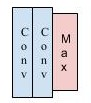
\includegraphics[scale=0.6]{Images/conv_block}
  \caption[\textgreek{Τμήμα Συνέλιξης}]{\textgreek{Τμήμα συνέλιξης: 2 επίπεδα συνέλιξης και ενα }Max-pooling \textgreek{επίπεδο.}}
 \label{fig:conv_block}
\end{figure}

\textgreek{Πιο συγκεκριμένα, στα επίπεδα συνέλιξης γεμίζουμε περιφερειακά την χαρτογράφηση των χαρακτηριστικών με μηδενικά ανάλογα με το μέγεθος του πυρήνα για να μπορέσουμε να κρατήσουμε το μέγεθος τους αναλλοίωτο κρατώντας την θέση των χαρακτηριστικών αλλά και επειδή χρειαζόμαστε την πληροφορία από τις γωνίες των χαρακτηριστικών. Η εικόνα }\ref{fig:conv_pad} \textgreek{μας δείχνει ένα παράδειγμα της διαδικασίας, ενώ η εξίσωση }\ref{eqn:half_pad} \textgreek{μας δείχνει ότι για να πετύχουμε μέγεθος εισόδου }(input) \textgreek{ίδιο με το μέγεθος εξόδου, πρέπει να ισχύει η παρακάτω εξίσωση, για οποιοδήποτε μέγεθος εισόδου }input \textgreek{και για μονό αριθμό στοιχείων πυρήνα $k$ όπου }($k = 2n + 1, n \in  \mathbb{N})$  \textgreek{, $s$ είναι το βήμα ολίσθησης το οποίο είναι 1 και δεν λαμβάνεται υπόψη στην εξίσωση. Με το }$p$ \textgreek{συμβολίζεται το γέμισμα των μηδενικών περιφερειακά της εισόδου όπου }$p = \lfloor k/2 \rfloor = n$.

\begin{equation}
\label{eqn:half_pad}
\begin{align*}
output &= input + 2\lfloor k/2 \rfloor -(k - 1) \\
        &= input + 2n - 2n \\
        &= input
\end{align*}
\end{equation}

\begin{figure}[H]
 \centering
 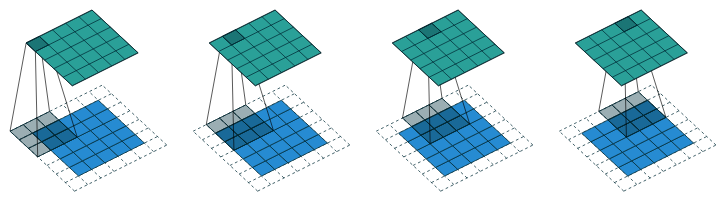
\includegraphics[scale=0.4]{Images/conv_pad}
  \caption[\textgreek{Συνέλιξη με }Zero-Padding]{\textgreek{Εφαρμογή ενός πυρήνα $3\times3$ με ολίσθηση μονού βηματισμού σε επίπεδο εισόδου μεγέθους $5\times5$ με γέμισμα μηδενικών περιφερειακά της εισόδου} \cite{conv_arithmetic}.}
 \label{fig:conv_pad}
\end{figure}


\textgreek{Το στάδιο κωδικοποίησης αποτελείται από 4 τμήματα (εικόνα }\ref{fig:conv_block})\textgreek{ όπου δέχεται σαν είσοδο την εικόνα μεγέθους $512\times512\times3$ και παράγει στην έξοδο μια χαρτογράφηση χαρακτηριστικών $32\times32\times256$, όπου η τρίτη διάσταση είναι ο αριθμός των φίλτρων. Πιο αναλυτικά στο πρώτο τμήμα έχουμε την συνέλιξη της εικόνας με μια σειρά από 32 φίλτρα και ακόμα ένα ίδιο επίπεδο πριν καταλήξουμε να εφαρμόσουμε το επίπεδο μέγιστης συγκέντρωσης. Το επίπεδο μέγιστης συγκέντρωσης είναι μια ανορθόδοξη τεχνική στην οποία επιδιώκουμε να μειώσουμε τον αριθμό των παραμέτρων σταδιακά, καθώς όσο προχωράμε στα επόμενα τμήματα αυξάνεται ο αριθμός του βάθους των επιπέδων (δηλαδή των φίλτρων) και επομένως και ο αριθμός των παραμέτρων. Ένας άλλος λόγος είναι η προσπάθεια της εξάλειψης της υπερμάθησης ως αποτέλεσμα της μείωσης των παραμέτρων. Στην δική μας περίπτωση συγκεντρώσαμε από κάθε περιοχή $2\times2$ την μέγιστη τιμή των χαρακτηριστικών. Συγκεκριμένα ολισθαίνουμε ένα παράθυρο μεγέθους $2\times2$ στα χαρακτηριστικά και παίρνουμε την μέγιστη τιμή. Διαισθητικά, αυτό σημαίνει ότι κρατήσαμε την τιμή που υπάρχει μεγαλύτερο ερέθισμα στον εκάστοτε νευρώνα (εικόνα }\ref{fig:maxpool}). \textgreek{Επομένως ο χάρτης των χαρακτηριστικών χώρου μετά από κάθε τμήμα μειώνεται κατά το ήμισυ, οι εξισώσεις παρακάτω μας δείχνουν τον υπολογισμό των διαστάσεων εξόδου μετά την εφαρμογή του επιπέδου μέγιστης συγκέντρωσης. Η μεταβλητή $P$ ορίζει τυχόν γέμισμα στο στάδιο της συγκέντρωσης το οποίο στην δική μας περίπτωση είναι μηδέν και με $S$ ορίζεται το άλμα ολίσθησης του πυρήνα συγκέντρωσης το οποίο είναι ίσο με 2.} 


\begin{equation}
  \label{eqn:maxpool}
  \begin{align*}
  Image &= H\times W \times D\\
  Height &= (Height - Pool size +2\times P)/S + 1\\
  Width &= (Width - Pool size +2\times P)/S + 1\\
  Output &= Height \times Width \times D
  \end{align*}
\end{equation}

\textgreek{Ο αλγόριθμος μέγιστης συγκέντρωσης εφαρμόζεται ανεξάρτητα σε κάθε φίλτρο εισόδου των χαρακτηριστικών. Δηλαδή δεν επηρεάζει το μέγεθος των φίλτρων καθώς εφαρμόζεται μόνο στις χωρικές διαστάσεις των χαρακτηριστικών.} 


\begin{figure}[H]
 \centering
 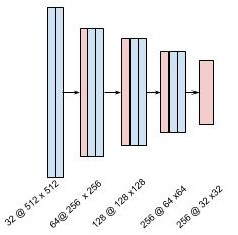
\includegraphics[scale=0.6]{Images/conv_enc}
  \caption[\textgreek{Στάδιο Κωδικοποίησης}]{\textgreek{Στάδιο κωδικοποίησης των ΣΝΔ} \textgreek{επίπεδο.}}
 \label{fig:encode_stage}
\end{figure}

\textgreek{Η εικόνα }\ref{fig:maxpool} \textgreek{μας δείχνει ένα παράδειγμα εφαρμογής ενός πυρήνα $3\times3$ πάνω σε ένα επίπεδο χαρακτηριστικών $5\times5$ εφαρμόζοντας την μέθοδο της μέγιστης συγκέντρωσης. Όπως βλέπουμε συγκεντρώνουμε το μέγιστο στοιχείο από τον $3\times3$ πυρήνα που ολισθαίνει σε όλο το επίπεδο ενός χάρτη χαρακτηριστικών, από αριστερά προς τα δεξιά.}

\begin{figure}[H]
 \centering
 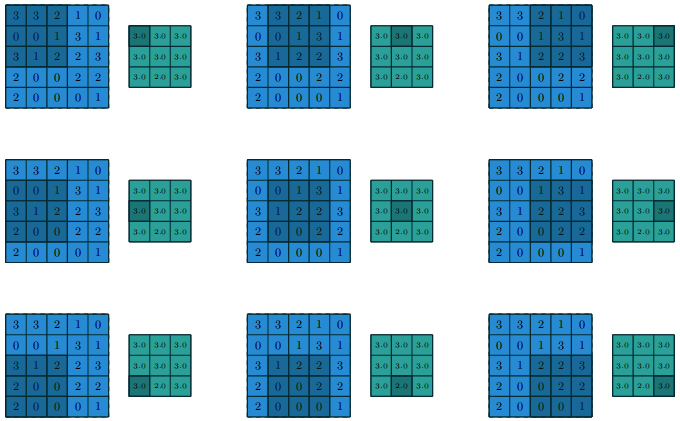
\includegraphics[scale=0.5]{Images/maxpool}
  \caption[\textgreek{Παράδειγμα Μέγιστη Συγκέντρωσης}]{\textgreek{Παράδειγμα της μεθόδου της μέγιστης συγκέντρωσης, εφαρμόζοντας ένα παράθυρο $3\times3$ σε ένα επίπεδο χαρακτηριστικών εισόδου $5\times5$ με μονό βήμα ολίσθησης. Τα βήματα είναι από αριστερά προς τα δεξιά} \cite{conv_arithmetic}.}
 \label{fig:maxpool}
\end{figure}

\subsection{\textgreek{Μονάδα Παράλληλης Επεξεργασίας Χαρακτηριστικών}}
\textgreek{Η παράλληλη μονάδα επεξεργασίας χαρακτηριστικών αποτελείται από 5 διαφορετικά τμήματα τα οποία δέχονται ως είσοδο τον χάρτη με τα κωδικοποιημένα χαρακτηριστικά από το στάδιο της κωδικοποίησης. Η εξίσωση }\ref{eqn:dilated_conv} \textgreek{μας δείχνει την συνέλιξη σε ένα επίπεδο σήμα εισάγοντας την διαστολή που υποδεικνύεται με $r$}.\textgreek{ Η συγκεκριμένη συνάρτηση υπάγεται στην θεωρία ως Διεσταλμένη Συνέλιξη} (Dilated Convolution) \textgreek{ενώ η εικόνα }\ref{fig:conv_ar_1} \textgreek{ μας δίνει μια διαίσθηση γύρω από αυτή την τεχνική.}

\begin{equation}
  \label{eqn:dilated_conv}
  g[i,j] = \sum_{k}\sum_{k} f[i+r\cdot k, j+r\cdot k]h[k,k] 
\end{equation}

\par
\textgreek{Πιο συγκεκριμένα, κάθε παρακλάδι της μονάδας επεξεργασίας διαφέρει στην διαστολή των στοιχείων του πυρήνα που αλληλεπιδρούν με την είσοδο (εικόνα }\ref{fig:parallel_unit}). \textgreek{Σκοπός αυτού του τμήματος είναι η μάθηση χαρακτηριστικών από διαφορετικά πεδία όρασης. Κάθε παρακλάδι διαθέτει έναν πυρήνα με διαφορετική διαστολή στο πρώτο επίπεδο. Ο πυρήνας σε όλους τους κλάδους έχει μέγεθος $3\times 3$, εκτός από το τελευταίο επίπεδο πριν την ένωση των χαρακτηριστικών όπου η πυρήνας έχει μέγεθος $1\times 1$. Στην εικόνα }\ref{fig:parallel_unit} \textgreek{βλέπουμε σε κάθε επίπεδο το μέγεθος κάθε επιπέδου και τον αριθμό του βάθους των φίλτρων τα οποία είναι 256, 128 και 128 αντίστοιχα. Ο λόγος που μειώνουμε τις διαστάσεις είναι για την μείωση των παραμέτρων κατά την εκπαίδευση. Επίσης, για να κρατήσουμε σταθερό το μέγεθος των χαρακτηριστικών και για να μην υπάρχει περαιτέρω αλλοίωση της πληροφορίας γεμίζουμε περιφερειακά με μηδενικά την είσοδο πριν την διαδικασία της συνέλιξης. Στο στάδιο της ένωσης πραγματοποιείται η πράξη της πρόσθεσης όλως των χαρακτηριστικών που καταλήγουν από κάθε κλάδο αντίστοιχα.}

\begin{figure}[H]
 \centering
 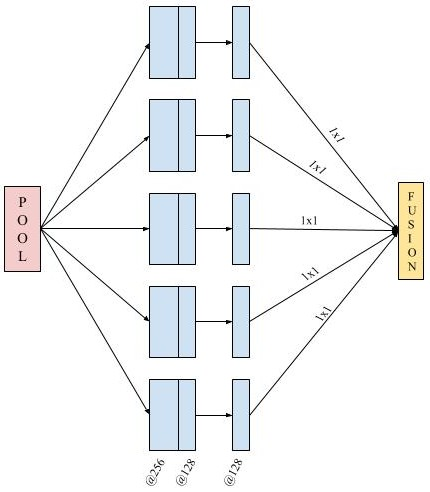
\includegraphics[scale=0.55]{Images/parallel_1}
  \caption[\textgreek{Παράλληλη Μονάδα Επεξεργασίας}]{\textgreek{Η παράλληλη μονάδα επεξεργασίας με τα 5 ξεχωριστά μονοπάτια. Το κάθε μονοπάτι έχει στο πρώτο επίπεδο συνέλιξης μια διαστολή: $3\times 3$, $6\times6$, $9\times9$, $12\times12$ και $1\times1$ αντίστοιχα. Επίσης, βλέπουμε και τον αριθμό των φίλτρων του κάθε επιπέδου συνέλιξης.} }
 \label{fig:parallel_unit}
\end{figure}


\textgreek{Παρακάτω βλέπουμε ένα παράδειγμα για την διεσταλμένη συνέλιξη όπου εφαρμόζουμε έναν πυρήνα $3\times3$ πάνω σε ένα επίπεδο εισόδου $7\times7$ με ολίσθηση του πυρήνα ίσο με 1 και χωρίς γέμισμα περιφερειακά της εισόδου με μηδενικά. Στην δική μας περίπτωση υπάρχει γέμισμα του χάρτη χαρακτηριστικών περιφερειακά με μηδενικά καθώς θέλουμε να κρατήσουμε το μέγεθος αναλλοίωτο αλλά και να προσπαθήσουμε να κρατήσουμε την θέση της πληροφορίας όσο περισσότερο γίνεται. 

\parΗ διεσταλμένη συνέλιξη γεμίζει τον πυρήνα του φίλτρου με μηδενικά ανάμεσα στα στοιχεία του πυρήνα. Για την ακρίβεια, για έναν ρυθμό διαστολής $\mathit{d}$ εισάγουμε $\mathit{d-1}$ μηδενικά ανάμεσα στα στοιχεία του πυρήνα και προφανώς για $d=1$ αναφερόμαστε σε μια τυπική συνέλιξη. Η συνέλιξη με διαστολή συνήθως χρησιμοποιείται για την αύξηση του δεκτικού πεδίου ενός νευρώνα χωρίς να χρειαστεί να αυξηθεί το μέγεθος του πυρήνα. Μία σημαντική ιδιότητα αυτής της τεχνικής είναι ο αριθμός των παραμέτρων ο οποίος αυξάνεται γραμμικά ενώ ο αριθμός του δεκτικού πεδίου αυξάνεται εκθετικά.}

\begin{figure}[H]
 \centering
 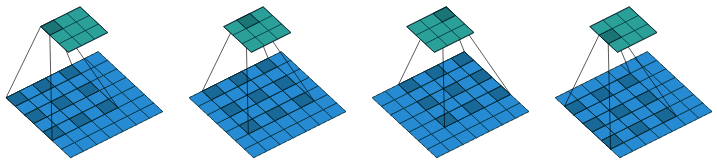
\includegraphics[scale=0.4]{Images/conv_ar_1}
 \caption[\textgreek{Διεσταλμένη Συνέλιξη}]{\textgreek{Συνέλιξη ενός πυρήνα μεγέθους $3\times3$ πάνω σε ένα επίπεδο εισόδου μεγέθους $7\times7$ και με διαστολή μεγέθους 2. Τα μπλε σκούρα στοιχεία δείχνουν την συμμετοχή για τον υπολογισμό της τιμής του στοιχείου (πράσινο σκούρο)} \cite{conv_arithmetic}. }
 \label{fig:conv_ar_1}
\end{figure}

\subsection{\textgreek{Στάδια Αποκωδικοποίησης}}
\subsubsection{\textgreek{Επισκόπηση}}
\textgreek{Παρακάτω θα εξηγήσουμε τις 2 παραλλαγές των μονάδων αποκωδικοποίησης που υλοποιήσαμε για να πειραματιστούμε με αυτές και να συγκρίνουμε τα αποτελέσματα τους στο πρόβλημα της Σημασιολογικής Κατάτμησης. Η κύρια διαφορά μεταξύ των 2 μονάδων είναι ο τρόπος που γίνεται η υπερδειγματοληψία. Η πρώτη μονάδα χρησιμοποιεί την μέθοδο της αποσυνέλιξης με εισαγωγή ενός βήματος για την επίτευξη της υπερδειγματοληψίας, ενώ στην δεύτερη μονάδα υλοποιήθηκε ένα επίπεδο διγραμμικής παρεμβολής που λειτουργεί με τον τρόπο που εξηγήσαμε στο τμήμα }\ref{sec:bilinear}.

\subsubsection{\textgreek{Μονάδα Αποσυνέλιξης Με Άλμα Ολίσθησης}}
\label{sec:sd-decoder}
\textgreek{Η συγκεκριμένη μονάδα αποκωδικοποίησης αποσκοπεί στην ανακατασκευή των χαρακτηριστικών από τον χάρτη χαρακτηριστικών πίσω στην μορφή της εικόνας. Η εικόνα }\ref{fig:deconv_1_stage} \textgreek{μας δείχνει την αρχιτεκτονική της μονάδας αποκωδικοποίησης. }

\begin{figure}[H]
 \centering
 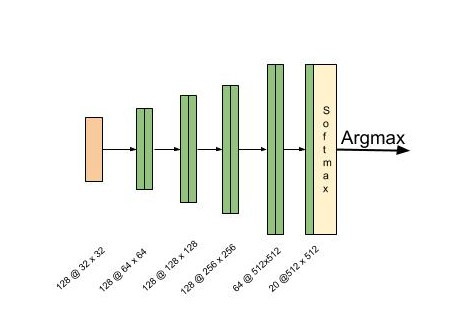
\includegraphics[scale=0.6]{Images/deconv_decoding}
  \caption[\textgreek{Στάδιο Αποκωδικοποίησης με βηματισμό}]{\textgreek{Στάδιο αποκωδικοποίησης του ΣΝΔ με χρήση επιπέδων αποσυνέλιξης.} }
 \label{fig:deconv_1_stage}
\end{figure}

\textgreek{Για να μπορέσουμε να εξηγήσουμε καλύτερα την μονάδα αποκωδικοποίησης θα πρέπει πρώτα να μιλήσουμε για την διαδικασία της αποσυνέλιξης ή ανάστροφης συνέλιξης όπως την βρίσκουμε στην βιβλιογραφία. Η ιδέα και η ανάγκη της ανάστροφης συνέλιξης προκύπτει από την επιθυμία να χρησιμοποιηθεί ένας μετασχηματισμός που να μας οδηγεί από τον χάρτη τον χαρακτηριστικών, δηλαδή στον μετασχηματισμό από ένα σχήμα κάποιου αντικειμένου πίσω στον ανασχηματισμό του σε σχέση με την εικόνα εισόδου. Με λίγα λόγια γίνεται μια ανακατασκευή της εικόνας από τα μεγάλων διαστάσεων χαρακτηριστικά. \par
Η τεχνική της ανάστροφης συνέλιξης μας οδηγεί από έναν χάρτη χαρακτηριστικών μικρού μεγέθους σε έναν χάρτη μεγαλύτερου μεγέθους ενώ συγκρατεί τα μοτίβα διασύνδεσης μεταξύ των νευρώνων. Η ανάστροφη συνέλιξη δουλεύει εναλλάσσοντας το μπροστινό πέρασμα με το πέρασμα της οπισθοδρόμησης της συνέλιξης. Με λίγα λόγια, η κανονική συνέλιξη με την ανάστροφη συνέλιξη είναι ο τρόπος με τον οποίο υπολογίζονται τα προς τα εμπρός και προς τα πίσω περάσματα }(feed-forward and backward passes). \par
\textgreek{Για παράδειγμα μπορεί ένας πυρήνας $\mathbf{w}$ να ορίζει μια συνέλιξη όπου τα περάσματα (εμπρός-πίσω) να υπολογίζονται από έναν πίνακα $\mathbf{C}$ και $\mathbf{C}^{T}$ αντίστοιχα, αλλά επίσης αν αναστρέψουμε τους πίνακες ορίζουμε την ανάστροφη συνέλιξη ορίζοντας τους πίνακες ως $\mathbf{C}^{T}$ και $(\mathbf{C}^{T})^{T} = \mathbf{C}$ για τα εμπρός και πίσω περάσματα αντίστοιχα. Τέλος, το τελευταίο επίπεδο πριν την εφαρμογή του επιπέδου} softmax \textgreek{έχουμε ένα επίπεδο με αριθμό βάθους χαρτών ίσο με 20, όσο είναι και οι κατηγορίες αντικειμένων. Κάθε επίπεδο του βάθους από τα 20 επίπεδα αποτελεί ένα }heatmap \textgreek{της κάθε κλάσης ως προς τις υπόλοιπες. Εφαρμόζοντας την }softmax \textgreek{μετασχηματίζεται η έξοδος σε μια κατανομή πιθανοτήτων. }   

\subsubsection{\textgreek{Διγραμμική Μονάδα Αποκωδικοποίησης}}

\textgreek{Η διγραμμική μονάδα αποκωδικοποίησης όπως βλέπουμε στην εικόνα }\ref{fig:bilinear_deconv} \textgreek{έχει πανομοιότυπη αρχιτεκτονική με την προηγούμενη μονάδα }\ref{sec:sd-decoder}, \textgreek{με την διαφορά στην μέθοδο που επιτυγχάνεται η υπερδειγματοληψία. Για την υπερδειγματοληψία του χάρτη χαρακτηριστικών χρησιμοποιείται η μέθοδος της διγραμμικής παρεμβολής. Κατά την διγραμμική παρεμβολή, ένα στοιχείο δημιουργείται από μια σταθμισμένη μέση τιμή από τέσσερα γειτονικά στοιχεία από τον χάρτη χαρακτηριστικών εισόδου. Το επίπεδο αυτό δεν διαθέτει παραμέτρους μάθησης. }

\begin{figure}[H]
 \centering
 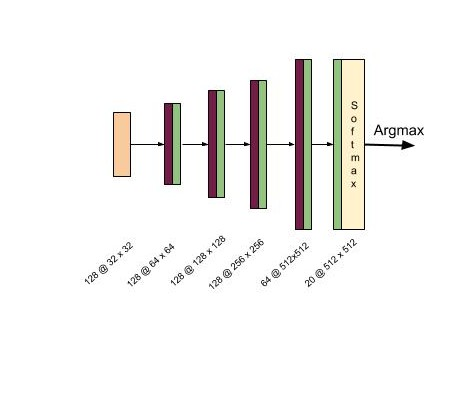
\includegraphics[scale=0.6]{Images/bilinear_conv}
  \caption[\textgreek{Διγραμμική Μονάδα Αποκωδικοποίησης}]{\textgreek{Στάδιο αποκωδικοποίησης του ΣΝΔ με χρήση επιπέδων διγραμμικής παρεμβολής για την υπερδειγματοληψία των χαρακτηριστικών. Τα μωβ επίπεδα υποδεικνύουν το επίπεδο της διγραμμικής παρεμβολής.}}
 \label{fig:bilinear_deconv}
\end{figure}
\pagebreak
\subsection{\textgreek{Ολοκληρωμένες Αρχιτεκτονικές}}
\textgreek{Η εικόνα }\ref{fig:systems} \textgreek{μας δείχνει τις μονάδες των αρχιτεκτονικών που περιγράψαμε προηγουμένως  μαζί με τις μονάδες μετά-επεξεργασίας που θα αναλύσουμε στο επόμενο κεφάλαιο. }

\begin{figure}[h]
\centering

\begin{subfigure}[b]{1\linewidth}
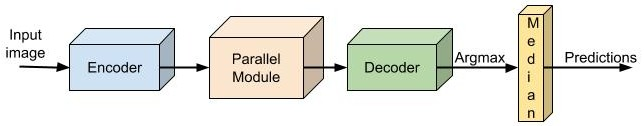
\includegraphics[scale=0.6]{Images/whole_arch_1}
 \caption{\textgreek{Ολοκληρωμένη αρχιτεκτονική με την μονάδα μετα-επεξεργασίας Μεσαίου Φίλτρου.}}
 \end{subfigure}
 \\[1cm]
 \begin{subfigure}[b]{1\linewidth}
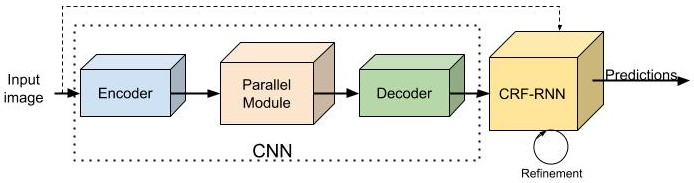
\includegraphics[scale=0.6]{Images/whole_arch_2}
\caption{\textgreek{Ολοκληρωμένη αρχιτεκτονική με την μονάδα μετα-επεξεργασίας ΤΥΣΠ-ΕΝΔ.}}
\end{subfigure}

\caption[\textgreek{Αρχιτεκτονικές ΣΝΔ}]{\textgreek{Ολοκληρωμένες Αρχιτεκτονικές.}}
\label{fig:systems}
\end{figure}



\chapter{\textgreek{Μονάδες Μετα-Επεξεργασίας}}

\pagestyle{fancy}
\fancyhf{}
%\fancyhead[OC]{\leftmark}
%\fancyhead[C]{}
%\fancyhead[EC]{\rightmark}
\renewcommand{\footrulewidth}{0.5pt}
\cfoot{\thepage}

\section{\textgreek{Επισκόπηση}}
\textgreek{Το πρόβλημα με τα Συνελικτικά Δίκτυα} (CNNs) \textgreek{είναι η προσαρμογή σε συνελικτικά φίλτρα με μεγάλα οπτικά πεδία όπως έχουμε και στην δική μας εργασία με τα διαφορετικά οπτικά πεδία που εφαρμόζονται στην παράλληλη μονάδα επεξεργασίας. Συνεπώς παράγουν χονδροειδείς εξόδους όταν αναδιαρθρώνονται για να παράγουν προβλέψεις σε επίπεδο εικονοστοιχείων και καταλήγουμε να έχουμε πιο γενικά όρια από ότι θα περιμέναμε. Επίσης, τα} CNNs \textgreek{δεν έχουν περιορισμούς ομαλότητας. Για να μπορέσουμε να διευθετήσουμε αυτό το πρόβλημα υιοθετήθηκαν δύο διαφορετικές προσεγγίσεις που θα εξηγήσουμε λεπτομερώς στα επόμενα τμήματα. Πρώτον ο αλγόριθμος Μέσου Φίλτρου που προσαρμόστηκε ως μονάδα μετα-επεξεργασίας και ο αλγόριθμος των Υποθετικών Τυχαίων Πεδίων ως Επαναλαμβανόμενα Νευρωνικά Δίκτυα} (CRFs as RNN). 

\section{\textgreek{Μεσαίο Φίλτρο}}
\textgreek{Ο αλγόριθμος του Μεσαίου Φίλτρου είναι μια μη γραμμική τεχνική ψηφιακού φιλτραρίσματος, που συχνά χρησιμοποιείται για την απομάκρυνση του θορύβου από μια εικόνα ή ένα σήμα. Μια τέτοια μείωση θορύβου είναι ένα τυπικό στάδιο προ-επεξεργασίας για τη βελτίωση των αποτελεσμάτων της μεταγενέστερης επεξεργασίας (για παράδειγμα, ανίχνευση ακμής σε μια εικόνα). Το μεσαίο φιλτράρισμα χρησιμοποιείται ευρέως στη ψηφιακή επεξεργασία εικόνων, επειδή υπό ορισμένες συνθήκες διατηρεί τις άκρες ενώ απομακρύνει τον θόρυβο έχοντας επίσης εφαρμογές στην επεξεργασία σήματος. 
\par 
Ο λόγος που χρησιμοποιήθηκε στα πειράματα μας είναι για να επιτύχουμε μια εξομάλυνση στις στην έξοδο του συστήματος, δηλαδή στις προβλέψεις του συστήματος για τα εικονοστοιχεία. Για παράδειγμα, αν μια περιοχή της εικόνας απεικονίζει έναν δρόμο, μπορεί να υπάρχουν ορισμένα εικονοστοιχεία που να έχουν προβλεφθεί ως πεζόδρομος, τότε με αυτό το φίλτρο θα πετύχουμε την μείωση των λανθασμένων εικονοστοιχείων της περιοχής της εικόνας. Η εξίσωση }\ref{eqn:median_filter} \textgreek{μας δείχνει την γενική εξίσωση της εφαρμογής ενός φίλτρου στην εικόνα, όπου  η τιμή του εικονοστοιχείου ($\mathit{g(i,j)}$) εξαρτάται από ένα σταθμισμένο άθροισμα των εικονοστοιχείων εισόδου ($\mathit{f(i+k,j+l)}$) και $\mathit{h(k,l)}$ ονομάζεται ο πυρήνας που περιέχει τους συντελεστές του φίλτρου }\cite{szeliski2011computer}.

\begin{equation}
    \centering
    \label{eqn:median_filter}
    g(i,j) = \sum_{k,l} f(i+k,j+l)h(k,l)
\end{equation}

\textgreek{Ο αλγόριθμος παρακάτω μας δείχνει βήμα-βήμα τον αλγόριθμο του Μεσαίου Φίλτρου:}

\begin{algorithm}[H]
    \caption{\textgreek{Αλγόριθμος Μεσαίου Φίλτρου} (Median Filter) \cite{wiki:median}.}
    \label{Algo_median}
  \begin{algorithmic}[2]
    \REQUIRE $\text{Output image} [W \times H]$
    \REQUIRE $\text{Input image} [W \times H]$
    \REQUIRE $Window [K \times K]$
    \REQUIRE $edgeX \gets round(K / 2)$
    \REQUIRE $edgeY \gets round(K / 2)$
    
    \FOR{\text{$x$ from edgeX to W - edgeX} }
      \FOR{\text{$y$ from edgeY to H - edgeY}}
	\STATE $i=0$
	\FOR{\text{Fx from 0 to K}}
	    \FOR{\text{Fy from 0 to K}}
		\STATE \text{$Window[i] = \text{Input image}[x + Fx - edgeX][y + Fy - edgeY]$}
		\STATE \text{$i \gets i + 1$}
	    \ENDFOR
	\ENDFOR
	\STATE \text{sort values in Window}
	\STATE \text{\text{Output Image}[x][y] $\gets$ Window[K * K / 2]}
     \ENDFOR
    \ENDFOR
    \RETURN \COMMENT{Output Image}

  \end{algorithmic}
\end{algorithm}
\textgreek{Ένα μειονέκτημα του αλγορίθμου είναι ότι για κάθε υπολογισμό ενός εικονοστοιχείου πρέπει να ταξινομήσουμε τα στοιχεία για να πάρουμε την ενδιάμεση τιμή. Επομένως, προσθέτει υπολογιστικό κόστος καθώς προσθέτει επιπλέον $\mathit{Ο(Ν^{2}})$ πράξεις.}

\section{\textgreek{Τυχαία υπό Συνθήκη Πεδία} (CRF)}
\textgreek{Τα Τυχαία υπό Συνθήκη Πεδία }(CRF) \textgreek{παρουσιάστηκαν ως μονάδα μετά-επεξεργασίας για την βελτίωση των αποτελεσμάτων. Χρησιμοποιούνται συνήθως σε προβλήματα σημασιολογικής κατάτμησης, ενώ ανήκουν στη κατηγορία των στατιστικών μοντέλων γράφων. Στην πραγματικότητα, πριν από την έλευση των νευρωνικών δικτύων και συγκεκριμένα των Συνελικτικών} (CNN), \textgreek{τα} CRF \textgreek{αποτελούσαν την καλύτερη δυνατή προσέγγιση σε θέματα σημασιολογικής κατάτμησης, ενώ πλέον χρησιμοποιούνται για βελτίωση αποτελεσμάτων καθώς τείνουν να βελτιώνουν την διαγράμμιση των ορίων των αντικειμένων στις εικόνες. Στην πραγματικότητα τα} CRF \textgreek{είναι ένα Τυχαίο Πεδίο} Markov (MRF) \textgreek{όπου οι συντελεστές του καθορίζονται από κάποιες συνθήκες στα δεδομένα.}


\subsection{\textgreek{Επισκόπηση Αλγορίθμου}}
\textgreek{Στην πραγματικότητα υπάρχουν πολλές παραλλαγές τέτοιων μοντέλων. Εμείς θα ασχοληθούμε με τα πυκνά μοντέλα} CRF \textgreek{και στην προκειμένη περίπτωση μια υλοποίηση που είναι βασισμένη σε επαναλαμβανόμενα νευρωνικά δίκτυα} (CRF as RNN). \textgreek{Θα δώσουμε μία συνοπτική περιγραφή του αλγορίθμου πριν προχωρήσουμε στην ανάλυση του. Τα }CRF \textgreek{όπως αναφέραμε, χρησιμοποιούνται για πρόβλεψη των εικονοστοιχείων, μοντελοποιούν τα εικονοστοιχεία ως τυχαίες κατανομές που δημιουργούν ένα }MRF \textgreek{όταν υπόκεινται σε μια μεγάλη κλίμακα παρατηρήσεων. Στην προκειμένη περίπτωση η μεγάλη κλίμακα παρατηρήσεων είναι η εικόνα. 
\par 
Ας υποθέσουμε ότι $X_{i}$ είναι μια τυχαία μεταβλητή που σχετίζεται με το εικονοστοιχείο $i$ το οποίο μπορεί να πάρει οποιαδήποτε τιμή από ένα σύνολο τιμών που ανήκει στο $\mathcal{L}$. Αν υποθέσουμε ότι $\mathbf{X}$ είναι το διάνυσμα των τυχαίων μεταβλητών $X_1,X_2,\dotsc,X_N$ όπου Ν ο αριθμός των εικονοστοιχείων της εικόνας. 
\par

Παίρνοντας σαν δεδομένο τον γράφο $\mathit{G = (V,E)}$ όπου $\mathit{V = {X_1,X_2,\dotsc,X_N}}$, μία παρατήρηση της εικόνας $\mathbf{I}$, το ζευγάρι $\mathbf{(I,X)}$ μπορεί να μοντελοποιηθεί ως μια κατανομή }Gibbs \textgreek{της μορφής $\mathit{P}(\mathbf{X}=\mathbf{x}|\mathbf{I}) = \frac{1}{Z(\mathbf{I})}\exp(-\mathit{E}\mathbf(x|I))$. Η συνάρτηση $\mathit{E(x)}$ είναι η ενέργεια των παρατηρήσεων $x \in \mathcal{L}^{N}$, ενώ η $Z(I)$ είναι η συνάρτηση διαμέρισης} (partition function) \cite{partition_func}. \textgreek{Στα πλήρως συνδεδεμένα }CRF \textgreek{ζεύγους }\cite{fully_crf} \textgreek{η ενέργεια της ανάθεσης ενός εικονοστοιχείου σε μια κατηγορία $\mathbf{x}$ δίνεται από την εξίσωση }\ref{eqn:energy}.

\begin{equation}
    \centering
    \label{eqn:energy}
    E(\mathbf{x}) = \sum_{i} \psi_{u}(x_{i}) + \sum_{i<j} \psi_{p}(x_{i},x_{j})
    %Q_{i}(l) \gets \frac{1}{Z_{i}} \exp(U_{i}(l))  \qquad \triangleright \text{Initialization} 
\end{equation}

\textgreek{Όπου $\psi_{u}(x_{i})$ είναι οι ενιαίοι συντελεστές ενέργειας οι οποίοι μετράνε την αντίστροφη πιθανότητα του εικονοστοιχείου $i$ να παίρνει την ετικέτα $x_{i}$ και οι συντελεστές ενέργειας ζεύγους $\psi_{p}(x_{i},x_{j})$ μετράνε το κόστος της ανάθεσης της τιμής $x_{i},x_{j}$ στα εικονοστοιχεία $i,j$ ταυτόχρονα.}

\begin{equation}
\centering
 \psi_{p}(x_{i},x_{j}) = \mu(x_{i},x_{j}) \displaystyle\sum_{m=1}^{M} w^{(m)}k_{G}^{(m)}(\mathbf{f}_{i},\mathbf{f}_j)
\end{equation}

\textgreek{Όπου $Κ_{G}^{(m)}$ (εξίσωση }\ref{eqn:gauss_kernel}) \textgreek{συνάρτηση η οποία αποτελείται από δύο Γκαουσιανύς Πυρήνες }(Gaussian Kernels) \textgreek{οι οποίοι εφαρμόζονται στα διανύσματα των στοιχείων }$\mathbf{f}_{i},\mathbf{f}_{j}$ \textgreek{τα οποία προέρχονται από τα χαρακτηριστικά της εικόνας, όπως πληροφορία θέσης των εικονοστοιχείων $(p)$ και τις τιμές των εικονοστοιχείων ($I$: }RGB values) \textgreek{και $w^{(m)}$ είναι τα βάρη των πυρήνων. Ο πρώτος πυρήνας εξαρτάται από την θέση και την τιμή των εικονοστοιχείων ενώ ο δεύτερος εξαρτάται αποκλειστικά από την θέση των εικονοστοιχείων. Οι παράμετροι $\theta_a$, $\theta_\beta$ και $\theta_\gamma$ χρησιμοποιούνται για την κανονικοποίηση των τιμών των πυρήνων. Η συνάρτηση $\mu(.,.)$ ονομάζεται συνάρτηση συμβατότητας, η οποία βρίσκει την συμβατότητα μεταξύ ενός ζεύγους εικονοστοιχείων ανάλογα με την ετικέτα που έχει ανατεθεί. Μειώνοντας την συνάρτηση ενέργειας παίρνουμε την πιο πιθανή τιμή (ετικέτα) στο $x$ δεδομένου μιας εικόνας. }

\begin{equation}
\label{eqn:gauss_kernel}
 k(\mathbf{f}_i,\mathbf{f}_j) = w^{(1)}\exp(-\frac{|p_i-p_j|^2}{2\theta^2_a }-\frac{|I_i-I_j|^2}{2\theta_\beta^2})+w^{(2)} \exp(-\frac{|p_i-p_j|^2}{2\theta^2_\gamma })
\end{equation}


\textgreek{Η εύρεση της ακριβής ελάχιστης τιμής δεν είναι εύκολο να υπολογιστεί καθώς δεν μπορούμε να υπολογίσουμε εύκολα την συνάρτηση διαμέρισης. Για αυτό τον σκοπό εφαρμόζεται η προσέγγιση Μέσου Πεδίου} (Mean-Field Approximation) \textgreek{στην κατανομή του }CRF, \textgreek{η παραπάνω διαδικασία γίνεται με την προσέγγιση της κατανομής $P(\mathbf{X})$ από μια απλούστερη κατανομή $Q(\mathbf X)$ η οποία μπορεί να γραφτεί σαν ένα γινόμενο ανεξάρτητων περιθωριακών κατανομών }$Q(\mathbf X) = \prod_{i} Q_{i}(X_{i})$. \textgreek{Παρακάτω θα δείξουμε αναλυτικά τα βήματα του αλγορίθμου και πως ο αλγόριθμος Μέσου Πεδίου μπορεί να αναδιαμορφωθεί σαν μια σειρά από πράξεις ενός ΣΝΔ (εικόνα} \ref{fig:cnn_mean_img})\textgreek{ και πως μοντελοποιείται σαν ένα ENΔ} (RNN) \cite{crf_as_rnn}.

\begin{figure}[H]
 \centering
 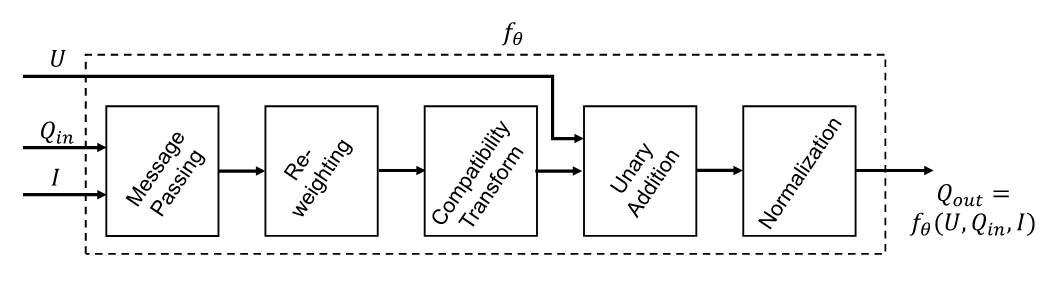
\includegraphics[scale=0.4]{Images/cnn_stack}
 \caption[MeanField as CNN]{\textgreek{Μία επανάληψη Μέσου Πεδίου ως }CNN \cite{crf_as_rnn}}
  \label{fig:cnn_mean_img}
\end{figure}

\subsection{\textgreek{Αρχικοποίηση}}
\textgreek{Στο πρώτο βήμα της αρχικοποίησης παρατηρούμε ότι στην ουσία έχουμε την εφαρμογή μιας συνάρτησης} softmax \textgreek{όπου } $Z_{i} = \sum_{l} exp(U_{i}(l))$ \textgreek{πάνω στις ενιαίες πιθανότητες} (Unary potentials). 
\\
\begin{equation}
    \label{init}
    \centering
    Q_{i}(l) \gets \frac{1}{Z_{i}} \exp(U_{i}(l))  \qquad \triangleright \text{Initialization} 
\end{equation}\\[1cm]

\subsection{\textgreek{Πέρασμα Μηνυμάτων}}
\textgreek{Στα πυκνά μοντέλα }CRF \textgreek{το πέρασμα μηνυμάτων πραγματοποιείται εφαρμόζοντας $M$ Γκαουσιανά Φίλτρα στις $Q$ κατανομές. Οι συντελεστές των φίλτρων προέρχονται από τα χαρακτηριστικά της εικόνας, όπως οι θέσεις και οι τιμές των εικονοστοιχείων, αλλά και πόσο έντονα ένα εικονοστοιχείο συσχετίζεται με ένα άλλο εικονοστοιχείο της εικόνας καθώς είναι όλα συνδεδεμένα μεταξύ τους. Επειδή ο υπολογισμός μεγάλων διαστάσεων Γκαουσιανών Φίλτρων είναι υπερβολικά μεγάλος, γίνεται η χρήση ενός αντιμεταθετικού πλέγματος} (Permutohedral lattice) \cite{lattice} \textgreek{το οποίο κάνει τον υπολογισμό των φίλτρων σε $O(N)$ χρόνο, όπου $N$ είναι το πλήθος των εικονοστοιχείων της εικόνας.} 
\par
\textgreek{Κατά τη διάρκεια της προς τα πίσω διάδοσης σφάλματος, οι είσοδοι των φίλτρων υπολογίζονται με την αποστολή των παραγώγων σφάλματος ως προς την έξοδο του φίλτρου μέσα από τα $M$ Γκαουσιανά Φίλτρα που θέσαμε αλλά με αντίστροφη κατεύθυνση. 
Επίσης, στο πλέγμα μία πολυδιάστατη συνέλιξη μπορεί να υλοποιηθεί ως μια ακολουθία από μονοδιάστατες συνελίξεις κατά μήκος των αξόνων του πλέγματος. Με αυτόν τον τρόπο το αντιμεταθετικό πλέγμα πετυχαίνει έναν πολύ αποδοτικό τρόπο περάσματος μηνυμάτων ανάμεσα στα εικονοστοιχεία.}

\begin{equation}
    \label{message}
    \centering
    %\tilde{Q}_{i}^{(m)}(l) \gets \sum_{j\neq i}
    \tilde{Q}_{i}^{(m)}(l) \gets \sum_{j\neq i} k^{(m)}(\mathbf{f}_{i},\mathbf{f}_{j})Q_{j}(l)  \qquad \triangleright \text{Message Passing} 
\end{equation}
\\[1cm]


\subsection{\textgreek{Στάθμιση Εξόδου Φίλτρου}}
\textgreek{Το επόμενο βήμα στον αλγόριθμο μέσου πεδίου λαμβάνει ένα σταθμισμένο άθροισμα των $Μ$ εξόδων φίλτρου από το προηγούμενο βήμα για κάθε ετικέτα κλάσης $l$. Όταν λαμβάνεται υπόψη κάθε ετικέτα κλάσης μεμονωμένα, μπορεί να θεωρηθεί ως μια συνέλιξη με μέγεθος φίλτρου 1 $\times$ 1 με $Μ$ κανάλια εισόδου και ένα κανάλι εξόδου. Επειδή και οι είσοδοι και οι έξοδοι σε αυτό το βήμα είναι γνωστές κατά τη διάρκεια της προς τα πίσω διάδοσης, η διαφορά σφάλματος ως προς τα βάρη του φίλτρου μπορεί να υπολογιστεί, καθιστώντας δυνατή την αυτόματη εκμάθηση των βαρών του φίλτρου.
\par 
Η παράγωγος του σφάλματος ως προς τις εισόδους μπορούν επίσης να υπολογιστούν με τον ίδιο τρόπο, να περάσουν οι παράγωγοι του σφάλματος προς τα πίσω, μέχρι το πρώτο στάδιο. Για να αποκτήσουμε μεγαλύτερο αριθμό ρυθμιζόμενων παραμέτρων, χρησιμοποιούμε ανεξάρτητα βάρη πυρήνα για κάθε ετικέτα κλάσης. Ο χωρικός πυρήνας και ο διμερής πυρήνας έχουν αντίθετες ιδιότητες και η συνεισφορά τους είναι σημαντική. Για παράδειγμα, οι διμερείς πυρήνες μπορεί από τη μία πλευρά να δίνουν έμφαση στην ανίχνευση ποδηλάτων καθώς η ομοιότητα των χρωμάτων είναι καθοριστική. Όμως, μπορεί να μην δίνουν σημασία για την ανίχνευση της τηλεόρασης, δεδομένου ότι οτιδήποτε βρίσκεται μέσα στην οθόνη της τηλεόρασης μπορεί να έχει πολλούς διαφορετικούς τύπους χρωμάτων.}\\[1cm]
\begin{equation}
    \label{eqn:weight}
    \centering
    %\tilde{Q}_{i}^{(m)}(l) \gets \sum_{j\neq i}
    \check{Q}_{i}(l) \gets \sum_{m} w^{(m)} \tilde{Q}_{i}^{(m)}(l)  \qquad \triangleright \text{Weighting Filter Outputs} 
\end{equation}
\\[1cm]

\subsection{\textgreek{Μετασχηματισμός Συμβατότητας}}
\textgreek{Στο βήμα Μετασχηματισμού Συμβατότητας, οι έξοδοι από το προηγούμενο βήμα (εξίσωση} \ref{eqn:weight})  \textgreek{μοιράζονται μεταξύ των ετικετών, ανάλογα φυσικά με τον βαθμό της συμβατότητας ανάμεσα στις ετικέτες. Η συμβατότητα μεταξύ των ετικετών των εικονοστοιχείων ορίζεται από την συνάρτηση $\mu(l,l')$.} \textgreek{Η οποία μαθαίνει την συμβατότητα μεταξύ δύο εικονοστοιχείων. Για παράδειγμα, η ανάθεση των ετικετών \emph{Άνθρωπος} και \emph{Ποδήλατο} έχουν μικρότερη ποινή από την ανάθεση των ετικετών \emph{ουρανός} και \emph{ποδήλατο}. Επίσης δεν ισχύει η μεταθετικότητα των ετικετών $\mu(l,l') \neq \mu(l',l)$. 
\par 
Η Συνάρτηση συμβατότητας μπορεί να θεωρηθεί ως ένα επιπλέον συνελικτικό επίπεδο όπου το μέγεθος του φίλτρου είναι $1\times1$ και ο αριθμός των καναλιών εισόδου και εξόδου είναι $L$. Μαθαίνοντας τα βάρη του φίλτρου είναι ισοδύναμο με την εκπαίδευση της συνάρτησης $\mathit{\mu}$ για τις ετικέτες των εικονοστοιχείων.}

\begin{equation}
    \label{compatible}
    \centering
    %\tilde{Q}_{i}^{(m)}(l) \gets \sum_{j\neq i}
    \hat{Q}_{i}(l) \gets \sum_{l'\in \mathcal{L}} \mu(l,l') \check{Q}_{i}(l')  \qquad \triangleright \text{Compatibility Transform} 
\end{equation}
\\[1cm]


\subsubsection{\textgreek{Πρόσθεση Πιθανοτήτων}}
\textgreek{Σε αυτό το βήμα, η έξοδος από τον Μετασχηματισμό Συμβατότητας αφαιρείται από τις ενιαίες πιθανότητες $U$. Εδώ δεν υπάρχουν παράμετροι, οπότε η διάδοση των διαφορών σφάλματος γίνεται απλά περνώντας τα από την έξοδο προς τις εισόδους.}

\begin{equation}
    \label{add}
    \centering
    \breve{Q}_{i}(l) \gets U_{i}(l) - \hat{Q}_{i}(l')  \qquad \triangleright \text{Adding Unary Potentials} 
\end{equation}
\\[1cm]

\subsection{\textgreek{Κανονικοποίηση}}
\textgreek{Τέλος όπως βλέπουμε στην εξίσωση} \ref{eqn:norm} \textgreek{έχουμε την κανονικοποίηση στο τέλος της επανάληψης όπου μπορεί να θεωρηθεί ως μια συνάρτηση} softmax \textgreek{χωρίς κάποιες παραμέτρους. Οι παράγωγοι από αυτό το βήμα περνάνε κανονικά προς την είσοδο μέσω της προς τα πίσω διάδοσης.}
\\[1cm]
\begin{equation}
    \label{eqn:norm}
    \centering
    %\tilde{Q}_{i}^{(m)}(l) \gets \sum_{j\neq i}
    {Q}_{i} \gets \frac{1}{Z_{i}} \exp(\breve{Q}_{i}(l)) \qquad \triangleright \text{Normalize} 
\end{equation}
\\[1cm]

\subsection{\textgreek{Τυχαία υπό Συνθήκη Πεδία ως Επαναλαμβανόμενα Νευρωνικά Δίκτυα} (CRF as RNN)}
\textgreek{Εδώ θα εξηγήσουμε πως η επαναληπτική διαδικασία του αλγορίθμου Μέσου Πεδίου μπορεί να μοντελοποιηθεί ως ένα Επαναλαμβανόμενο Νευρωνικό Δίκτυο. 
\par 
Χρησιμοποιούμε την $\mathit{f_{\theta}}$ για να υποδείξουμε την συνάρτηση μεταφοράς που προκύπτει από μια επανάληψη μέσου πεδίου. Δοθέντος μιας εικόνας $Ι$, καθώς και τις ενιαίες πιθανότητες $U$ και την εκτίμηση των περιθωριακών πιθανοτήτων $Q_{in}$ από την προηγούμενη επανάληψη, η επόμενη εκτίμηση των πιθανοτήτων δίνεται από τον εξής τύπο: $f_{\theta}(U,Q_{in},I)$. Το διάνυσμα $\mathbf{\theta} = \{w^{m},\mu(l,l')\}, \mu \in \{1,\cdots,M\},$ και $ l,l' \in \{l_{1},\cdots l_L\}$ αναπαριστούν τις παραμέτρους του }CRF \textgreek{που περιγράψαμε προηγουμένως.}
\par 
\textgreek{Οι επαναλήψεις του αλγορίθμου του Μέσου Πεδίου υλοποιούνται ως μια στοίβα από επίπεδα με τέτοιο τρόπο ώστε σε κάθε επανάληψη να παίρνει τις εκτιμήσεις $Q$ της προηγούμενης επανάληψης και τις ενιαίες πιθανότητες $U$ από το }CNN. \textgreek{Αυτή η διαδικασία που ακολουθείται είναι ίδια με την διαδικασία που ακολουθούν τα }RNN \textgreek{για εκπαίδευση. Οι εξισώσεις } \ref{eqn:H_eq_1}, \ref{eqn:H_eq_2} \textgreek{και} \ref{eqn:H_eq_3} \textgreek{μας δείχνουν την διαδικασία της επανεκτίμησης των πιθανοτήτων, όπου $Τ$ είναι ο αριθμός των επαναλήψεων του Μέσου Πεδίου} (Mean-Field Iterations):

%%%%%%%%%%%%%% H(t) Functions %%%%%%%%%%%%%%%%%%%5555
\begin{equation}
  H_{1}(t) = 
\begin{cases}
     softmax(U), \qquad t = 0\\
     H_{2}(t-1), \qquad 0< t \leq T
\end{cases}
\label{eqn:H_eq_1}
\end{equation}

\begin{equation}
  H_{2}(t) = f_{\theta}(U,H_{1}(t),I), \qquad 0 \leq t \leq T
 \label{eqn:H_eq_2}
\end{equation}

\begin{equation}
  Y(t) = 
\begin{cases}
     0, \qquad 0 \leq t < T\\
     H_{2}(t), \qquad t=T
\end{cases}
 \label{eqn:H_eq_3}
\end{equation}
%%%%%%%%%%%%%%%%%%%%%%%%%%%%%%%%%%%%%%%%%%%%%%%%%%%%%%%%%%%%%
\textgreek{Οι παράμετροι του μοντέλου }(CRF-RNN) \textgreek{είναι ίδιες με τις παραμέτρους του αλγορίθμου Μέσου Πεδίου και αναφέρονται ως $\mathit{\Theta}$. Επομένως, ο υπολογισμός των διαφορών του σφάλματος ως προς τις παραμέτρους είναι μια επανάληψη Μέσου Πεδίου, μπορούν να εκπαιδευτούν σαν Επαναλαμβανόμενο Νευρωνικό Δίκτυο με τον αλγόριθμο της Προς τα Πίσω Διάδοσης μέσω Χρόνου} (Back Propagation Through Time-BPTT) \cite{bptt_1, bptt_2}.

\begin{figure}[H]
 \centering
 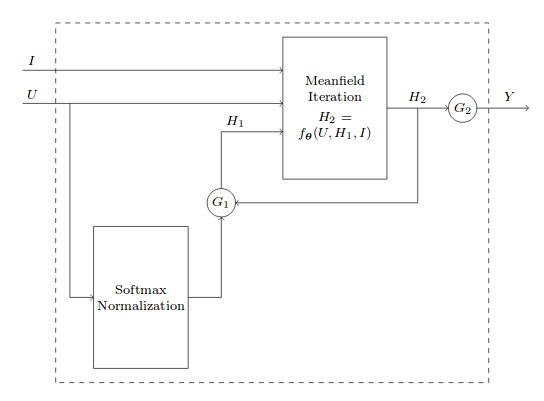
\includegraphics[scale=0.6]{Images/crf_as_rnn}
 \caption[CRF-RNN Network]{\textgreek{Ο επαναληπτικός αλγόριθμος Μέσου Πεδίου ως ένα επαναλαμβανόμενο νευρωνικό δίκτυο. Οι συναρτήσεις} $G_{1}, G_{2}$ \textgreek{είναι απλά οι συναρτήσεις εξόδου} \cite{crf_as_rnn}.}
  \label{fig:crf_rnn}
\end{figure}

\textgreek{Στην εικόνα} \ref{fig:crf-rnn-complete} \textgreek{βλέπουμε την ολοκληρωμένη αρχιτεκτονική, στο δικό μας μοντέλο οι ενιαίες πιθανότητες }(Unary potentials $\mathit U$) \textgreek{είναι η έξοδος από το τελευταίο επίπεδο του ΠΣΝΔ όπως φαίνεται στην εικόνα.}

\begin{figure}[H]
 \centering
 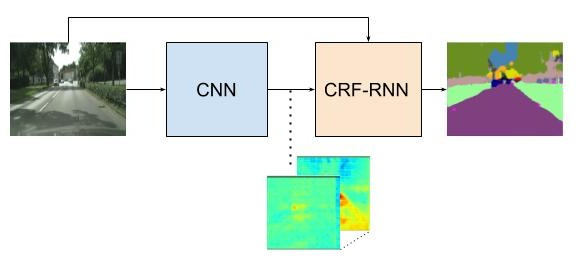
\includegraphics[scale=0.6]{Images/crf-rnn-mine}
 \caption[CNN CRF-RNN Network]{\textgreek{Ολοκληρωμένη αρχιτεκτονική του ΠΣΝΔ μαζί με το ΤΥΣΠ-ΕΝΔ. Το ΤΥΣΠ-ΕΝΔ δέχεται ως είσοδο την κανονική εικόνα μαζί με τις ενιαίες πιθανότητες του ΠΣΝΔ.}}
 \label{fig:crf-rnn-complete}
\end{figure}
%\chapter{}
\chapter{\textgreek{Πειράματα και Αποτελέσματα}}
\label{chapter_5}
\pagestyle{fancy}
\fancyhf{}
%\fancyhead[OC]{\leftmark}
%\fancyhead[C]{}
%\fancyhead[EC]{\rightmark}
\renewcommand{\footrulewidth}{0.5pt}
\cfoot{\thepage}

\section{\textgreek{Εκπαίδευση των Νευρωνικών Δικτύων}}
\textgreek{Σε αυτο το κομμάτι θα παρουσιάσουμε μερικές τεχνικές τις οποίες εφαρμόσαμε για την εκπαίδευση των ΠΣΝΔ καθώς και κάποιες υπερ-παραμέτρους που θέσαμε κατά την διαδικασία της εκπαίδευσης. Η εκπαίδευση των ΠΣΝΔ αποτελεί μια χρονοβόρα διαδικασία και επειδή μπορεί να πάρει μέρες για να συγκλίνει, κρίναμε απαραίτητη την τοποθέτηση κάποιων σημείων ελέγχου κατά την διαδικασία της εκπαίδευσης. }

\subsection{\textgreek{Σημεία Ελέγχου} (Checkpoints)}
\textgreek{Τα σημεία ελέγχου αποτελούν ένα απαραίτητο κομμάτι για την διαδικασία της εκπαίδευσης, ειδικά όταν έχουμε ΠΣΝΔ βαθειάς μάθησης. Η διαδικασία της μάθησης μπορεί να πάρει πολύ χρόνο, όπως στην δική μας περίπτωση που ήταν μερικές μέρες μέχρι να φτάσουμε σε σύγκλιση. Επομένως, πρέπει να αποθηκεύουμε τις παραμέτρους που μαθαίνει το ΠΣΝΔ κατά την μάθηση για να μην συμβεί κάποια αστοχία και χρειαστεί να κάνουμε την διαδικασία της μάθησης από την αρχή.
\par
Για το δικό μας μοντέλο θέσαμε ως σημείο ελέγχου το τέλος της κάθε εποχής} (epoch),\textgreek{ όπου αποθηκεύουμε τις παραμέτρους μας σε περίπτωση που χρειαστεί να συνεχίσουμε την εκπαίδευση του ΠΣΝΔ από εκείνο το σημείο. Ο όρος 'Εποχή' αντιπροσωπεύει την τροφοδοσία ενός ΝΔ με το σύνολο δεδομένων εκπαίδευσης. Η διαδικασία η οποία ολόκληρο το σύνολο δεδομένων εκπαίδευσης περνά μία φορά από το στάδιο της εμπρόσθιας διάδοσης και της οπισθοδρόμησης αντίστοιχα ορίζεται ως 'Εποχή'.  Ιδανικά, στο τέλος κάθε εποχής ελέγχουμε τα αποτελέσματα της μάθησης, επομένως αν υπάρχει κάποια βελτίωση στην διαδικασία της μάθησης, ελέγχοντας την ακρίβεια του μοντέλου στο σύνολο δεδομένων επαλήθευσης που χρησιμοποιούμε }(validation set) \textgreek{στο τέλος κάθε εποχής τότε αποθηκεύουμε τα βάρη του. }

\subsection{\textgreek{Πρώιμο Σταμάτημα} (Early Stopping)}
\textgreek{Το πρώιμο σταμάτημα είναι ένας μηχανισμός ο οποίος αποσκοπεί στην αποδοτικότητα της εκπαίδευσης του ΠΣΝΔ. Αποσκοπεί στην αποτροπή του μοντέλου από την κατάσταση της υπερ-μάθησης }(over-fitting). \textgreek{Ελέγχουμε το σφάλμα από το σύνολο επαλήθευσης σε κάθε εποχή, αν δεν υπάρχει κάποια μείωση του σφάλματος για 12 συνεχόμενες εποχές, τότε σταματάει η διαδικασία της μάθησης. Με αυτόν τον τρόπο σταματάει η διαδικασία της μάθησης πριν το μοντέλο αρχίσει να μαθαίνει υπερβολικά το σύνολο δεδομένων της εκπαίδευσης το οποίο αποτελεί πρόβλημα.}

\subsection{\textgreek{Ρυθμός Μάθησης}}
\textgreek{Ο ρυθμός μάθησης είναι από τις πιο σημαντικές παραμέτρους για την εκπαίδευση των ΝΝ. Χρειάζεται να είναι μικρό το μέγεθος για να συγκλίνει, αλλά όχι πολύ μικρό ώστε να πάρει πάρα πολύ χρόνο να βρεθεί σε σύγκλιση. Για την εκπαίδευση των ΣΝΔ βρήκαμε την βέλτιστη τιμή του ρυθμού μάθησης να είναι $10^{-3}$ χρησιμοποιώντας τον αλγόριθμο} Adam \textgreek{ ως αλγόριθμο βελτιστοποίησης. Ενώ για την εκπαίδευση του ΣΝΔ μαζί με το ΤΥΣΠ-ΕΝΔ βρήκαμε σαν βέλτιστη επιλογή την χρήση ενός πολύ μικρότερου ρυθμού μάθησης το οποίο ήταν $10^{-13}$ σε συνδυασμό με τον αλγόριθμο βελτιστοποίησης} SGD \textgreek{και με χρήση της παραμέτρου της ορμής επιλεγμένη στο 0.9. Για την ακρίβεια, ξεκινήσαμε με ρυθμό μάθησης $10^{-6}$ και σταδιακά δοκιμάστηκαν και μικρότεροι ρυθμοί μάθησης μέχρι να καταλήξουμε στο $10^{-13}$. }



\section{\textgreek{Αποτελέσματα}}
\textgreek{Τα μοντέλα εκπαιδεύτηκαν σε 2975 εικόνες μεγέθους $512\times 512$ η κάθε μία, ενώ το σύνολο των εικόνων επαλήθευσης το οποίο χρησιμοποιούμε για την επαλήθευση του μοντέλου στο τέλος της κάθε εποχής είναι 500 εικόνες. Επίσης οι εικόνες έχουν επαληθευτεί στο κανονικό τους μέγεθος ($1024\times 2048$). Τα μοντέλα εκπαιδεύτηκαν σε παρτίδες }(batches) \textgreek{όπου το μέγεθος ήταν 2 και 4 εκτός από την ολοκληρωμένη εκπαίδευση του }end-to-end \textgreek{μοντέλου ΠΣΝΔ-ΤΥΣΠ-ΕΝΔ που χρησιμοποιήθηκε μέγεθος ίσο με ένα λόγω των περιορισμένων διαθέσιμων πόρων. Τα αποτελέσματα στον πίνακα }\ref{table:results_table_1} \textgreek{μας δείχνουν τις επιδόσεις των ΠΣΝΔ σε συνδυασμό με την μονάδα επεξεργασίας Μέσου Φίλτρου καθώς δοκιμάζουμε τις επιδόσεις με διαφορετικό μέγεθος παραθύρου, ενώ ο πίνακας }\ref{table:results_table_2} \textgreek{επιδεικνύει τις επιδόσεις του μοντέλου με μονάδα μετα-επεξεργασίας ΤΥΣΠ-ΕΝΔ καθώς και την σύγκριση με τις αναδρομικές επαναλήψεις κατά την δοκιμή. Η δοκιμή του μοντέλου έγινε στα δεδομένα επαλήθευσης, δηλαδή στις 500 εικόνες.} 


\textgreek{Η μετρική που χρησιμοποιούμε στα αποτελέσματα είναι ένας μέσος όρος του πλήθους των επιτυχών προβλέψεων του μοντέλου ως προς το άθροισμα των λανθασμένων προβλέψεων του μοντέλου μαζί με τα $TP$ για την κάθε εικόνα. Πιο συγκεκριμένα μετράμε συνολικά από όλη την εικόνα τις παραμέτρους }$TP, FP, FN$ \textgreek{και υπολογίζουμε την συνάρτηση $J$. Επομένως μετράμε την συνάρτηση }Jaccard Similarity ($J$) \textgreek{(εξίσωση }\ref{eqn:jaccard}) \textgreek{ή} Intersection over Union \textgreek{από κάθε εικόνα και παίρνουμε έναν μέσο όρο από τις 500 εικόνες που χρησιμοποιήσαμε για την δοκιμή του μοντέλου (εξίσωση} \ref{eqn:mean_jaccard}). \textgreek{Επίσης, κατά την μέτρηση του μοντέλου δεν λάβαμε υπόψη μας τα εικονοστοιχεία τα οποία είναι ταξινομημένα ως 'Κενά'. Δηλαδή, αν ένα εικονοστοιχείο έχει ταξινομηθεί σε μία οποιαδήποτε κλάση $i$ και ανήκει στην κλάση 'Κενό' τότε δεν συνεισφέρει στο αποτέλεσμα.}

\noindent\begin{minipage}{.5\linewidth}
  \begin{equation}
  \label{eqn:jaccard}
    \begin{split}
  J &= \frac{TP}{TP+FP+FN}\\[1cm]
  TP &= \texttt{True Positives}\\ 
  FP &= \texttt{False Positives}\\
  FN &= \texttt{False Negatives}\\
  \end{split}
  \end{equation}
\end{minipage}%
\begin{minipage}{.5\linewidth}
  \begin{equation}
  \label{eqn:mean_jaccard}
  mIoU = \frac{1}{N}\sum_{i=1}^{N} J(i)
  \end{equation}
\end{minipage}
  
%%%%%%% ΕΔΩ ΚΑΤΩ Ο ΚΑΚΟΣ ΧΑΜΟΣΣΣΣΣΣΣ %%%%%%%%%%%%%%%%%%%%%%%%%%%%%%
True Positives \textgreek{συμβολίζονται τα εικονοστοιχεία τα οποία έχουν προβλεφθεί σωστά από τον ταξινομητή. Από την σκοπιά της στατιστικής, } False Positives \textgreek{είναι όταν το μοντέλο που έχει προβλέψει ένα αποτέλεσμα απορρίπτει την αναγνώριση του σωστού αποτελέσματος λανθασμένα. Ενώ }False Negatives \textgreek{είναι όταν το μοντέλο λανθασμένα απέτυχε να απορρίψει το αποτέλεσμα που πρόβλεψε.} 
\par 
%%%%%%%%%%%%%%%%%%%%%%%%%%%%%%%%


  

\begin{table}[H]
 \begin{adjustwidth}{-0.8cm}{}
\scalebox{0.8}{
\begin{tabular}{l|llllllllll}
\hline
\textbf{Model}     & - & 9x9  & 19x19    & 31x31 & 45x45 & 59x59 & 65x65 & 71x71 & 77x77 & 81x81 \\ \hline
SD-CNN-MFB & 0.607106 & 0.60792& 0.60847& 0.60905& 0.60960 & 0.60997 & \textbf{0.60998}& 0.60989& 0.60976& 0.60957\\ 
SD-CNN     &0.76681 & 0.76711& \textbf{0.76716}  & 0.76684& 0.76574& 0.76380& 0.76265& 0.76136 & 0.75996& 0.75897\\%\hline
SD-CNN-CRF[3] & 0.62051 & 0.62132& 0.62186& 0.62251& 0.62316& 0.62352& \textbf{0.62355} & 0.62345& 0.62322& 0.62303\\
BD-CNN     & 0.80342 & 0.80360 & \textbf{0.80373}& 0.80351  & 0.80234& 0.80001 & 0.79857& 0.79695& 0.79509 & 0.79375 \\

\end{tabular}
}
\caption[\textgreek{Αποτελέσματα Μέσου Φίλτρου}]{\textgreek{Αποτελέσματα των ΠΣΝΔ με τον αλγόριθμο Μέσου Φίλτρου ως μονάδα μετα-επεξεργασίας χρησιμοποιώντας διαφορετικά μεγέθη παραθύρων.} SD (Strided Deconvolution) \textgreek{είναι η μονάδα με αποκωδικοποίησης με βήμα ολίσθησης ενώ }BD (Bilinear Deconvolution) \textgreek{είναι η διγραμμική μονάδα αποκωδικοποίησης. Με }MFB (Median Frequency Balance) \textgreek{συμβολίζουμε την συνάρτηση ισοστάθμισης που χρησιμοποιήσαμε.}}\label{table:results_table_1}
\end{adjustwidth}
\end{table}

\textgreek{Όπως φαίνεται στον πίνακα }\ref{table:results_table_1} \textgreek{το μεσαίο φίλτρο δεν προσδίδει ιδιαίτερη βελτίωση στα αποτελέσματα παρά μόνο μια μικρή εξομάλυνση. Για την ακρίβεια η βελτίωση είναι της τάξης του $0.2\%$. }
\par
\textgreek{Τα μοντέλο }SD-CNN \textgreek{το οποίο εκπαιδεύτηκε με την συνάρτηση ισοστάθμισης μέσης συχνότητας πήρε 70 εποχές μέχρι να επιτευχθεί σύγκλιση καθώς επειδή προσπαθεί το ΣΝΔ να μάθει πληροφορία από όλες τις κλάσεις ανεξάρτητα της δυσαναλογίας χρειάζεται περισσότερο χρόνο για την σύγκλιση εφόσον η λανθασμένη ταξινόμηση ενός εικονοστοιχείου που βρίσκεται σε μια σπάνια κατηγορία διαδίδει μεγαλύτερο σφάλμα προς τα πίσω στο ΣΝΔ. Τα ΣΝΔ που εκπαιδεύτηκαν χωρίς ισοστάθμιση, χρειάστηκαν μόνο 40 εποχές για να συγκλίνουν καθώς βρέθηκαν πολύ γρήγορα σε κατάσταση υπερμάθησης.}
\par

\textgreek{Ο πίνακας} \ref{table:results_table_2} \textgreek{δείχνει την επίδοση του μοντέλου }SD-CNN \textgreek{μαζί με την μονάδα μετα-επεξεργασίας ΤΥΣΠ-ΕΝΔ} (CRF-RNN). \textgreek{Αρχικά επιχειρήσαμε να παγώσουμε την μάθηση στο ΠΣΝΔ και να γίνει η εκπαίδευση μόνο στο ΤΥΣΠ-ΕΝΔ όμως δεν υπήρχε κάποιο θετικό αποτέλεσμα. Εν τέλει, ξεκινήσαμε να εκπαιδεύσουμε το ΠΣΝΔ σε συνδυασμό με το ΤΥΣΠ-ΕΝΔ αρχικά με 10 επαναλήψεις και με ρυθμό μάθησης $10^{-6}$ για να δούμε την ανταπόκριση του μοντέλου. Σταδιακά μειώσαμε τον ρυθμό μάθησης σε $10^{-13}$ όμως ακόμα και μετα από 20 εποχές το μοντέλο άρχισε να αποκλίνει. Πιθανότητα λόγω των πολλών επαναλήψεων στο ΤΥΣΠ-ΕΝΔ παρουσιάστηκε το φαινόμενο της εξαφάνισης των αποκλίσεων. Επομένως μειώσαμε τον αριθμό των επαναλήψεων σε 5 κατά την μάθηση και πετύχαμε σύγκλιση μετα από 30 εποχές.
\par 
Το πρόβλημα με τους γράφους είναι ότι στηρίζονται πάρα πολύ στον ταξινομητή (ΣΝΔ) που τα τροφοδοτεί για να συνεισφέρουν περισσότερο στην επίδοση. Στην προκειμένη περίπτωση πετύχαμε μια βελτίωση της τάξης του 1\%. Από τον πίνακα }\ref{table:results_table_2} \textgreek{είναι ολοφάνερο πως όσο αυξάνονται οι επαναλήψεις επιβαρύνεται με επιπλέον χρόνο το μοντέλο καθώς σε κάθε επανάληψη γίνεται επανεκτίμηση της κατανομής. Για περισσότερες από 3 επαναλήψεις το μοντέλο δεν παρουσιάζει κάποια βελτίωση, επίσης στον πίνακα βλέπουμε και τον χρόνο της συμπερασματολογίας καθώς και μια τυπική απόκλιση του χρόνου σε δευτερόλεπτα που μετρήσαμε από την συμπερασματολογία 500 εικόνων.}

\begin{table}[H]
\centering
\begin{tabular}{lccc}
\hline
\textbf{Model[Iterations]}  & \textbf{mean IoU} & \textbf{\textgreek{Χρόνος  Διεκπεραίωσης}[s]} & \textbf{\textgreek{Απόκλιση Χρόνου}} \\ \hline
SD-CNN      & 0.60710            & 0.1111              & 0.06               \\ %\hline
SD-CNN-CRF{[}3{]}  & 0.62058              & 0.3988              & 0.09               \\ %\hline
SD-CNN-CRF{[}5{]}  & 0.62051            & 0.6994              & 0.17               \\ %\hline
SD-CNN-CRF{[}10{]} & 0.62051            & 1.1868              & 0.09               \\ %\hline
SD-CNN-CRF{[}20{]} & 0.62051 & 2.5681 & 0.48 \\

\end{tabular}

\caption[\textgreek{Αποτελέσματα} CNN-CRF]{\textgreek{Σύγκριση των μοντέλων με την μονάδα μετα-επεξεργασίας ΤΥΣΠ-ΕΝΔ με διαφορετικό αριθμό επαναλήψεων.}}\label{table:results_table_2}
\end{table}


\textgreek{Στον πίνακα }\ref{table:results_table_3} \textgreek{βλέπουμε την ακρίβεια του μοντέλου μας σε σχέση με τα σύγχρονα μοντέλα στο }test set \textgreek{του συνόλου δεδομένων. Για τα αποτελέσματα χρησιμοποιήθηκε η μετρική }IoU \textgreek{της εξίσωσης }\ref{eqn:jaccard} \textgreek{με την διαφορά ότι υπολογίστηκε για κάθε κλάση και ο μέσος όρος βγήκε από τον αριθμό των κλάσεων που υπάρχουν σε κάθε εικόνα. Στην δεξιά στήλη βλέπουμε την ακρίβεια που είχαν τα μοντέλα στην σωστή ταξινόμηση των εικονοστοιχείων σε μια από της εφτά υπερ-κατηγορίες. Το σύνολο δεδομένων αποτελείται από $1525$ εικόνες, ενώ η αξιολόγηση έγινε στον }server \textgreek{της βάσης }Cityscapes \cite{Cityscapes}. \textgreek{Ο πίνακας }\ref{table:results_table_4} \textgreek{μας δείχνει την ακρίβεια των μοντέλων για την αναγνώριση της κάθε κατηγορίας.}

\begin{table}[H]
\centering
\begin{tabular}{lccc}
\hline
\textbf{Model}  & \textbf{mean IoU Class} & \textbf{mean IoU Category}\\ \hline
PSPNet \cite{pspnet}  & 80.2     & 90.2   \\ %\hline
ResNet-DUC-HDC \cite{duc_hdc} & 80.1 & -\\
GRN-LRN-ResNet \cite{DBLP:conf/ijcai/ZhangTLLY17} & 77.27& - \\
PEARL-ResNet101 \cite{video_scene_parsing}& 74.9 & -\\ %\hline
RefineNet-ResNet101 \cite{RefineNet}& 73.06    & -         \\ %\hline
AdapNet \cite{adapNet}& 72.91 & -\\
SD-CNN-CRF{[}3{]} (Ours)  & 34.08  &  60.15  \\ %\hline
\end{tabular}

\caption[\textgreek{Σύγκριση με σύγχρονα μοντέλα}]{\textgreek{Σύγκριση του μοντέλου μας με σύγχρονα μοντέλα στο }test set.}\label{table:results_table_3}
\end{table}

\textgreek{Τα περισσότερα μοντέλα που κατέχουν τις πρώτες θέσεις διαθέτουν πολύ βαθιά ΣΝΔ με εκατοντάδες εκατομμύρια παραμέτρους εν αντιθέσει με το δικό μας μοντέλο το οποίο διαθέτει μόλις $7$ εκατομμύρια. Το }PSPNet \textgreek{για παράδειγμα διαθέτει ένα προ-εκπαιδευμένο ΣΝΔ }(ResNet) \textgreek{με $101$ επίπεδα συνέλιξης το οποίο είχε εκπαιδευτεί πρώτα σε ένα άλλο σύνολο δεδομένων }(ImageNet) \textgreek{και αποσκοπούσε στην εξαγωγή πολύπλοκων χαρακτηριστικών για την τροφοδοσία του ΣΝΔ }(PSPNet) \textgreek{ το οποίο πέτυχε την πρώτη θέση στην κατάταξη.}

\begin{table}[H]
  \begin{adjustwidth}{-1.5cm}{}
  \scalebox{0.55}{
    \begin{tabular}{l|ccccccccccccccccccc}
      \hline
      \textbf{Model}  & road & sidewalk & building& wall &fence & pole &traffic light&traffic sign & vegetation &terrain &sky & person &rider &car & truck &bus & train & motorcycle & bicycle \\ \hline
SD-CNN-CRF{[}3{]} & 86.99  &  44.03 & 60.00 & 14.35 & 9.20 & 9.60 & 10.86 & 10.54 & 70.72 & 49.31 & 81.04 &27.55& 18.26 &71.99&10.51&18.33&21.49&7.13 &25.64  \\ %\hline
    \end{tabular}}
    \caption[\textgreek{Αποτέλεσμα μοντέλου ανά κατηγορία}]{\textgreek{Αποτελέσματα για κάθε κατηγορία από τον }server \textgreek{της βάσης με την μετρική} IoU (\%).}\label{table:results_table_4}
  \end{adjustwidth}
\end{table}

\textgreek{Όπως μπορούμε να δούμε από τον πίνακα }\ref{table:results_table_5} \textgreek{βλέπουμε ότι τα αποτελέσματα σε επίπεδο υπερ-κατηγορίας είναι αρκετά ανεβασμένα. Αυτό μας δείχνει ότι το μοντέλο μπερδεύει περισσότερο τα εικονοστοιχεία τα οποία βρίσκονται στην ίδια υπερ-κατηγορία. Αντιθέτως, τα αποτελέσματα για τις υπερ-κατηγορίες 'Αντικείμενο' }(object) \textgreek{και 'Άνθρωπος'} (human) \textgreek{είναι αρκετά χαμηλά. Μια εξήγηση σε αυτό είναι η αναλογία των εικονοστοιχείων που ανήκουν σε αυτές τις υπερ-κατηγορίες σε σχέση με τα υπόλοιπα εικονοστοιχεία. Τα εικονοστοιχεία που ανήκουν στις παραπάνω υπερ-κατηγορίες είναι πολύ λιγότερα σε σχέση με τα υπόλοιπα και αυτή η μεγάλη δυσαναλογία δεν μπορεί να αντιμετωπιστεί εύκολα από την μέθοδο ισοστάθμισης κλάσεων. Επίσης τα αντικείμενα που ανήκουν σε αυτές τις κατηγορίες είναι πιο δύσκολο να αναγνωριστούν στην εικόνα.}

\begin{table}[H]
 \begin{tabular}{l|ccccccc}
  \hline
  \textbf{Model} & flat & nature & object & sky & construction & human & vehicle \\ \hline
    SD-CNN-CRF{[}3{]} & 93.42 & 71.01 & 14.67 & 81.04 & 60.19 & 30.60 & 70.15
 \end{tabular}
  \caption[\textgreek{Αποτέλεσμα ανά υπερ-κατηγορία}]{\textgreek{Αποτελέσματα μοντέλου ανά υπερ-κατηγορία στο }test set.}\label{table:results_table_5}
\end{table}


\textgreek{Παρακάτω βλέπουμε μερικές εκτιμήσεις πάνω σε εικόνες από τα μοντέλα που παρουσιάσαμε. Στην εικόνα }\ref{fig:image_results_1} \textgreek{βλέπουμε τα αποτελέσματα από μια εικόνα εισόδου στο μοντέλο }SD-CNN-CRF \textgreek{το οποίο έχει εκπαιδευτεί με ισοστάθμιση κλάσεων. Σε γενικές γραμμές έχει καταφέρει να τμηματοποιήσει αρκετά από τα αντικείμενα αν και όχι στη πιο λεπτομερή μορφή. Ο λόγος πιθανότητα που υπάρχει μια αστοχία και μια υπερκατάτμηση σε αντικείμενα όπως οι πινακίδες κυκλοφορίας και τα φανάρια κυκλοφορίας είναι η συμπίεση που υπέστη το μοντέλο από τα τμήματα συγκέντρωσης τα οποία χάνουν αρκετή πληροφορία ενώ τα επίπεδα υπερδειγματοληψίας φαίνεται να μην μπορούν να ανταπεξέλθουν σε αυτό το πρόβλημα. Επίσης, το μεσαίο φίλτρο ομαλοποιεί κάπως κάποια απομακρυσμένα εικονοστοιχεία από την κατηγορία τους τα οποία έχουν ταξινομηθεί σε λάθος κατηγορία.} 
\newpage
\textgreek{Στην εικόνα }\ref{fig:image_results_2} \textgreek{βλέπουμε το ίδιο μοντέλο ΠΣΝΔ με προηγουμένως χωρίς να έχει εκπαιδευτεί με κάποια συνάρτηση ισοστάθμισης. Αυτό είναι προφανές καθώς το ΠΣΝΔ έχει μάθει πολύ λιγότερες κατηγορίες, δηλαδή τις επικρατέστερες κατά πλειοψηφία. Αν και το ΠΣΝΔ έχει μάθει αρκετά καλά τις επικρατέστερες κλάσεις, γενικά αδυνατεί να αναγνωρίσει οποιαδήποτε άλλη κλάση.}\par

\textgreek{Τέλος, στην εικόνα }\ref{fig:image_results_3} \textgreek{βλέπουμε ένα δείγμα από το μοντέλο με την διγραμμική αποκωδικοποίηση το οποίο δεν έχει εκπαίδευση με την συνάρτηση για την δυσαναλογία των κλάσεων. Κάτι που παρατηρούμε είναι πως αν και χωρίς ισοστάθμιση κλάσεων καταφέρνει να αναγνωρίσει περισσότερα εικονοστοιχεία στην εικόνα εισόδου που ανήκουν και σε κλάσεις που αποτελούν μειονότητα. Μια εξήγηση για αυτό είναι ότι το προηγούμενο μοντέλο διαθέτει περισσότερες παραμέτρους λόγω του τμήματος υπερδειγματοληψίας που διαθέτει με εκπαιδευόμενες παραμέτρους τείνει να πάσχει από μεγαλύτερο πρόβλημα υπερμάθησης.}


%%%% IMAGE PREDICTIONS
\begin{figure}[H]
 \centering
 \begin{subfigure}[b]{\linewidth}
  \centering
  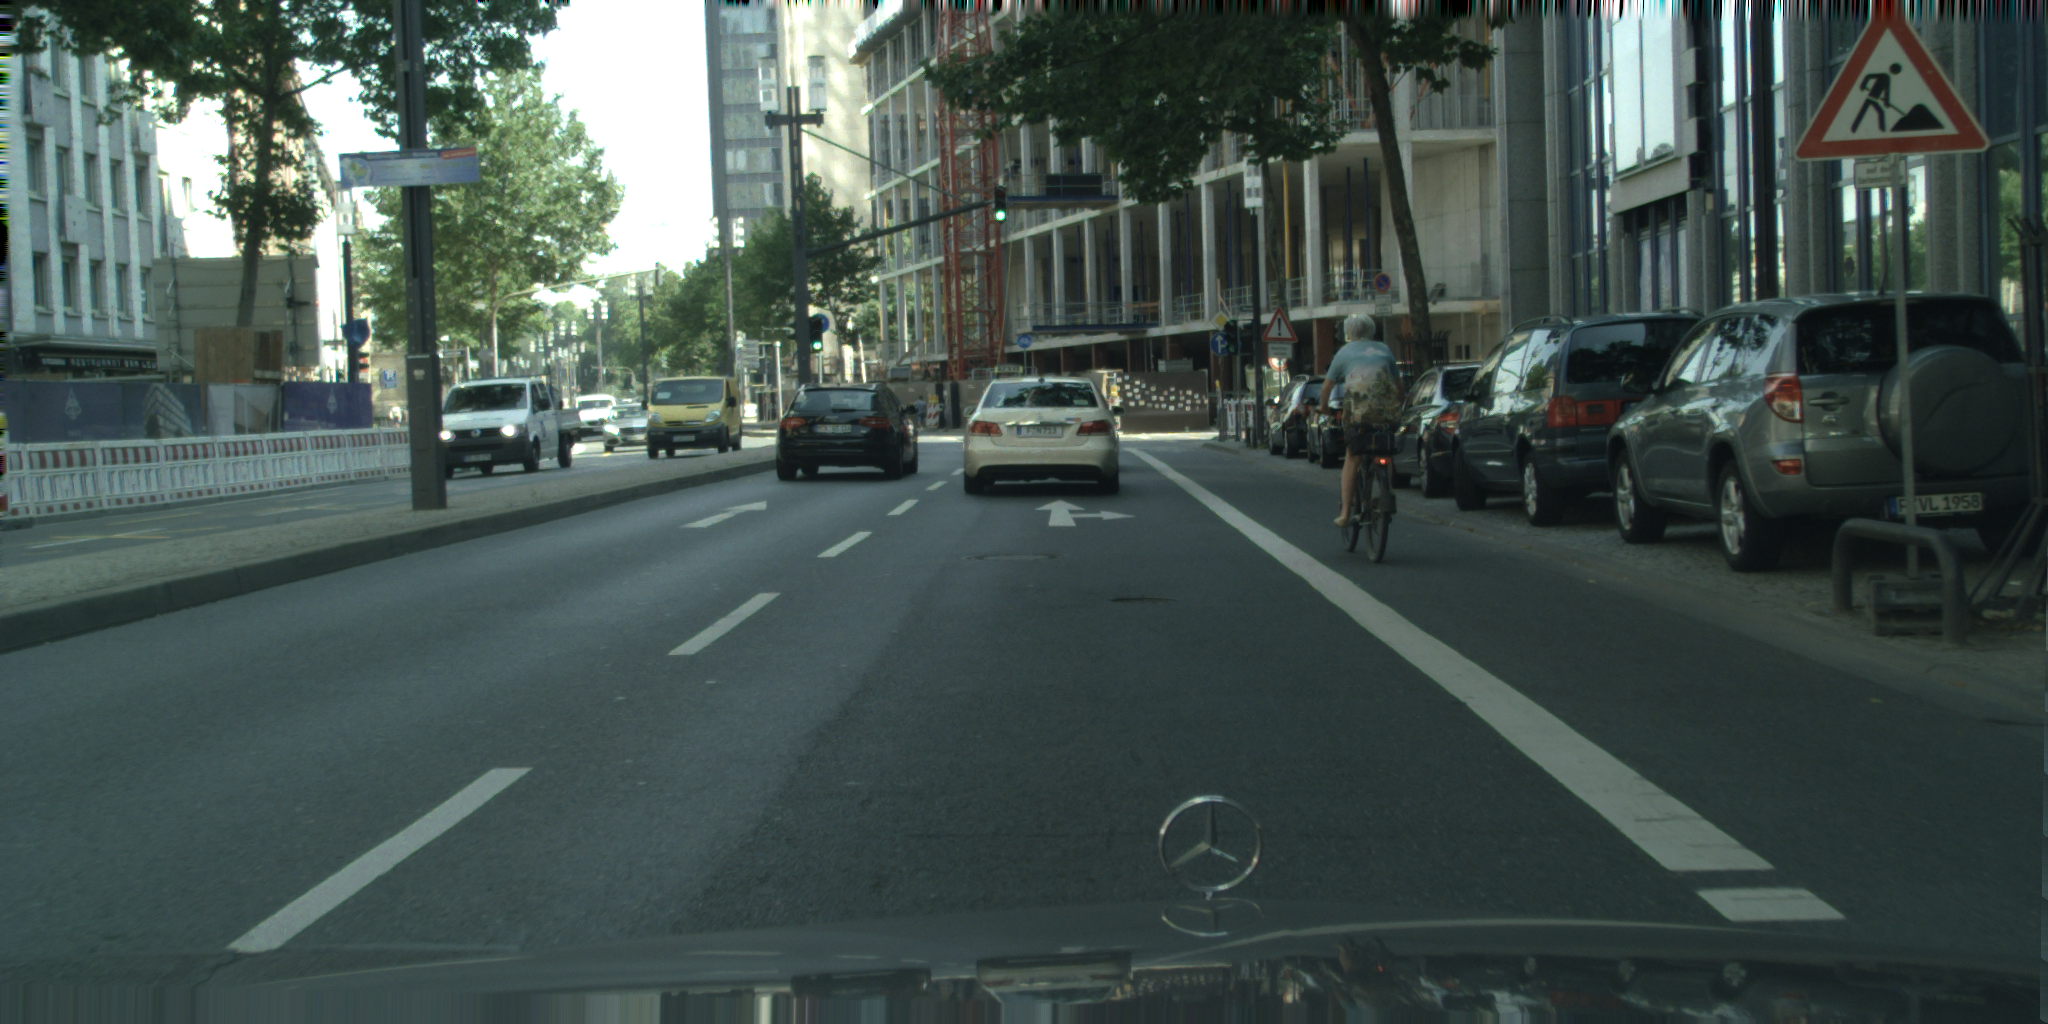
\includegraphics[width=0.67\linewidth]{Images/Original_frankfurt_000000_015676_leftImg8bit}
  \caption{\textgreek{Εικόνα εισόδου}}
  \end{subfigure}
 
 \begin{subfigure}[b]{\linewidth}
  \centering
  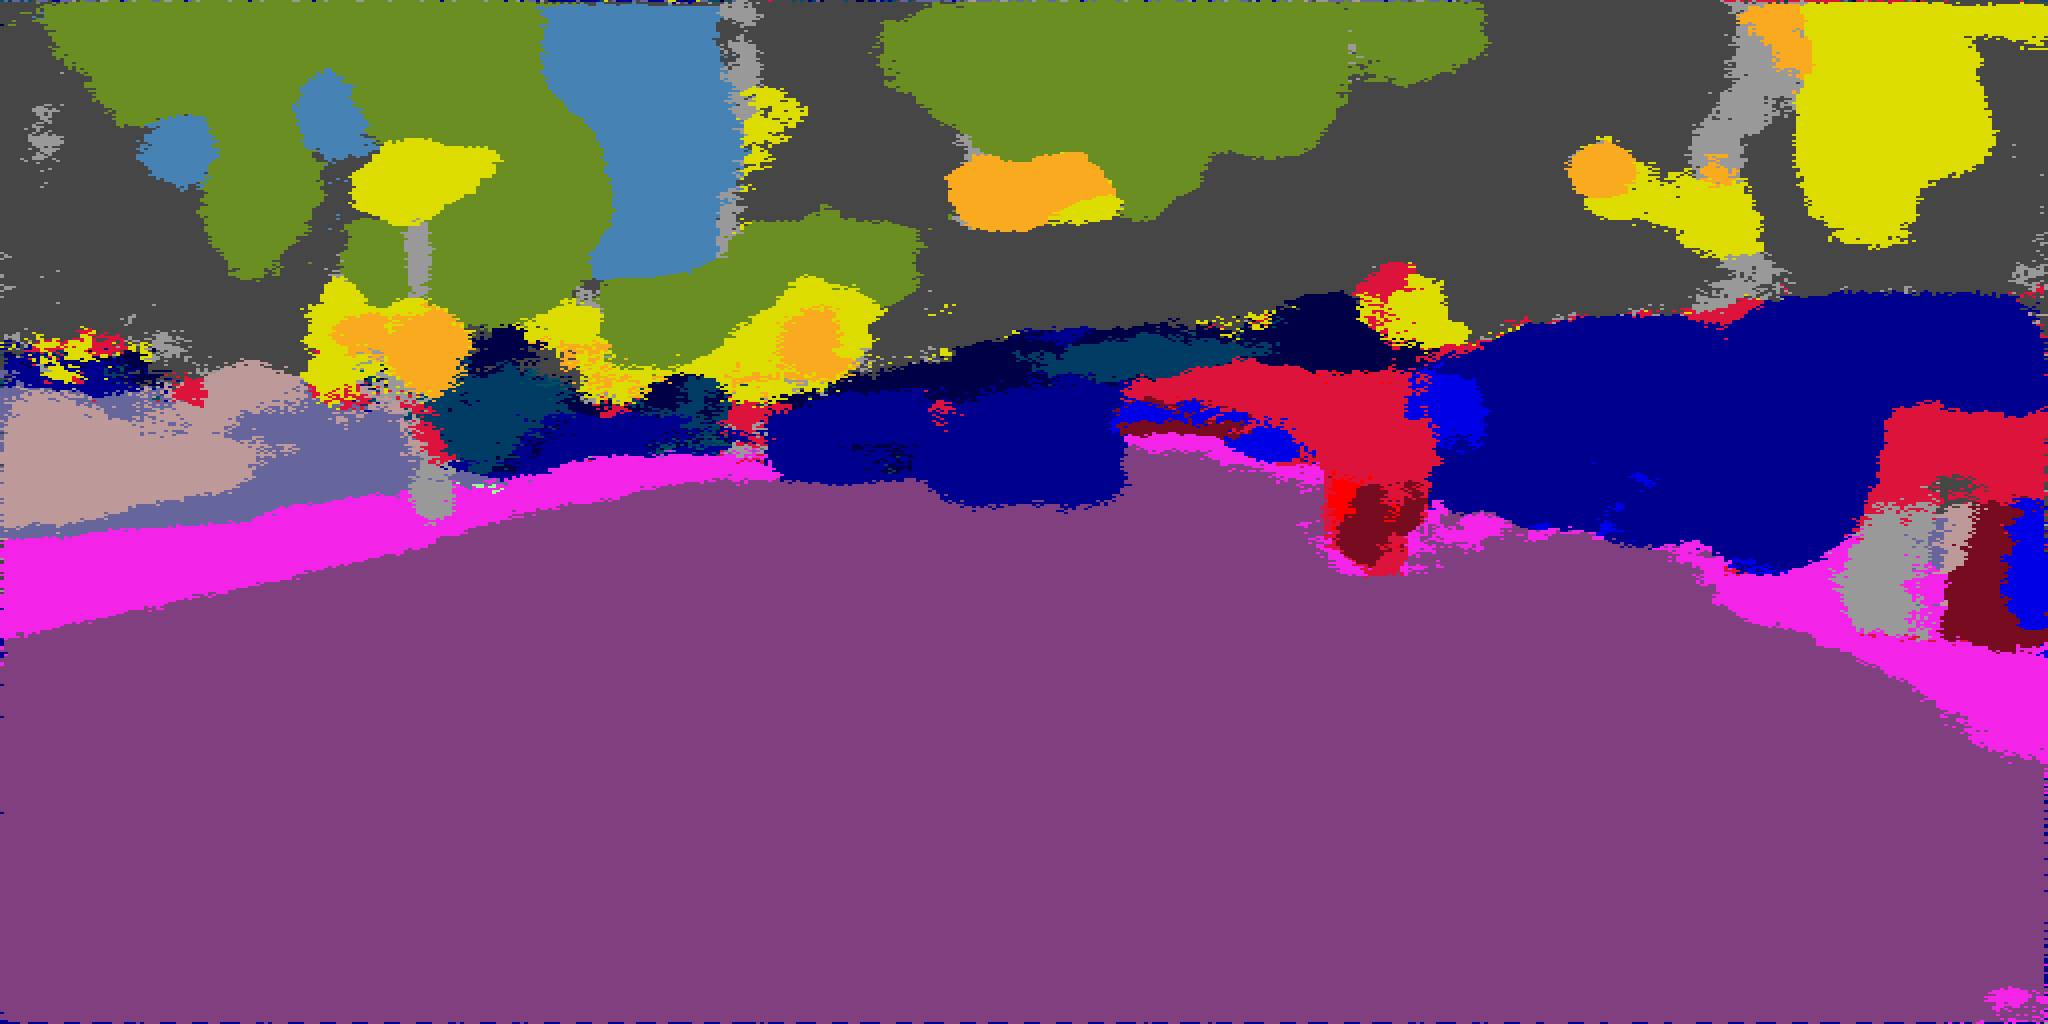
\includegraphics[width=0.67\linewidth]{Images/frankfurt_000000_015676_leftImg8bit_7_10_1024}
  \caption{\textgreek{Πρόβλεψη μοντέλου }SD-CNN-CRF-RNN.}
 \end{subfigure}
  
 \begin{subfigure}[b]{\linewidth}
  \centering
  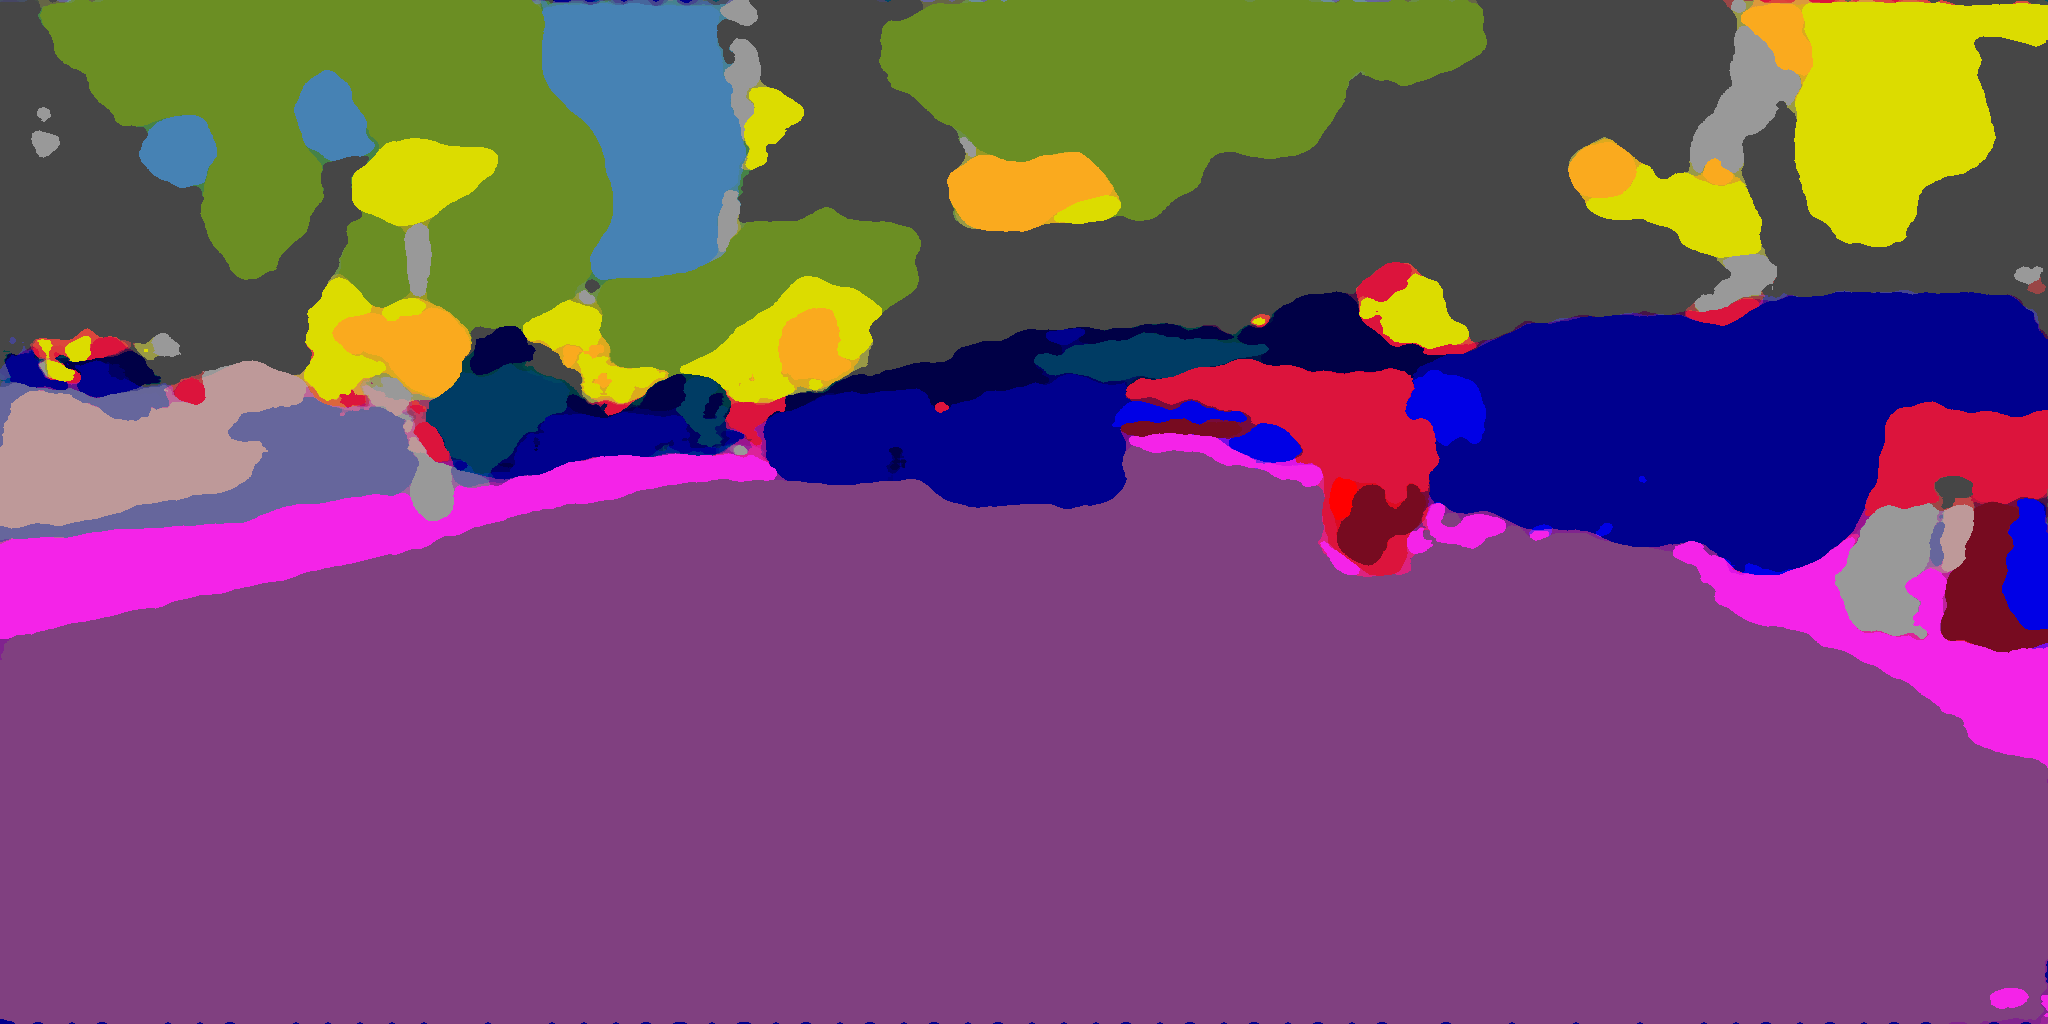
\includegraphics[width=0.67\linewidth]{Images/frankfurt_000000_015676_leftImg8bit_median_7_10_1024}
  \caption{\textgreek{Πρόβλεψη μοντέλου }SD-CNN-CRF-RNN \textgreek{με μεσαίο φίλτρο}.}
 \end{subfigure}
  
 \begin{subfigure}[b]{\linewidth}
  \centering
  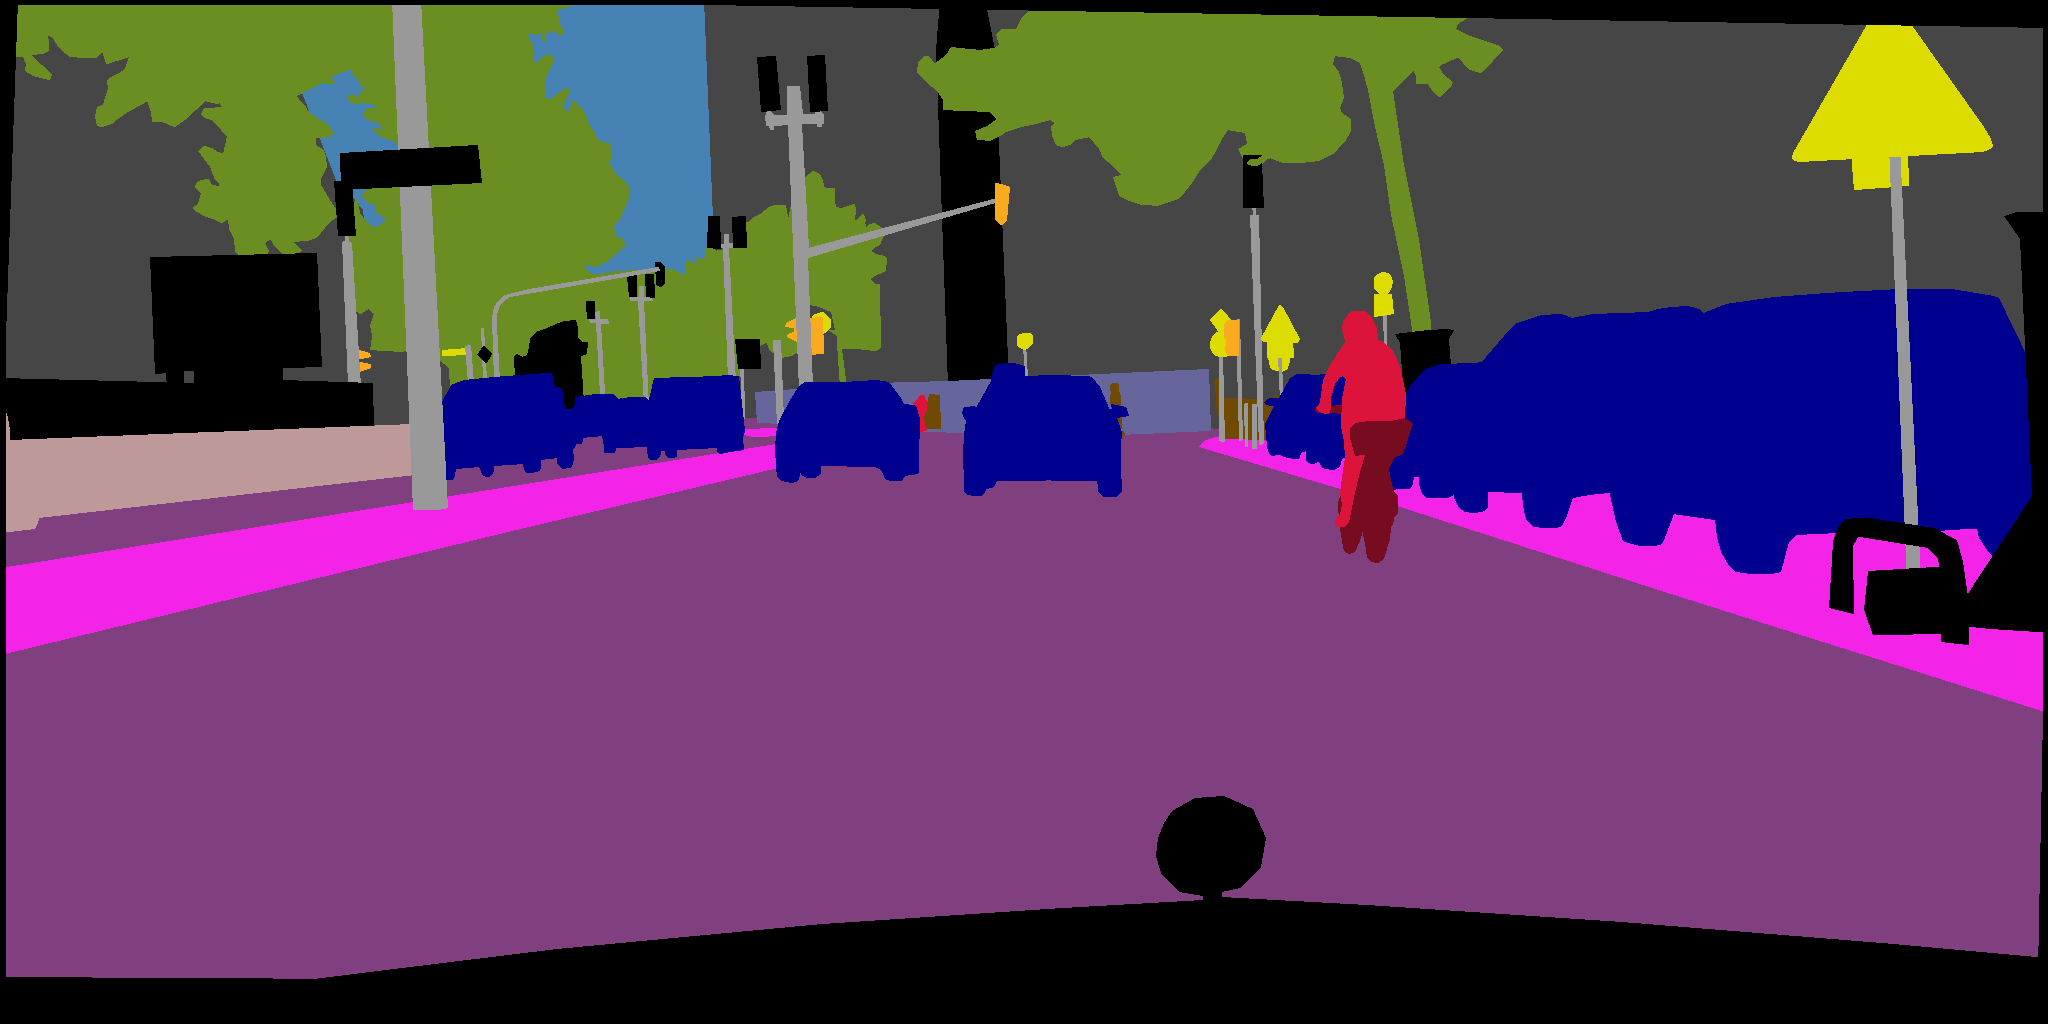
\includegraphics[width=0.67\linewidth]{Images/frankfurt_000000_015676_gtFine_color}
  \caption{Ground Truth}
 \end{subfigure}
  
  \caption[\textgreek{Εικόνες από ΠΣΝΔ-ΤΥΣΠ-ΕΝΔ}]{\textgreek{Εικόνες αποτελεσμάτων του ΠΣΝΔ με ΤΥΣΠ-ΕΝΔ με ισοστάθμιση κλάσεων.}}
 \label{fig:image_results_1}
\end{figure}

\begin{figure}[H]
 \centering
 \begin{subfigure}[b]{\linewidth}
 \centering
 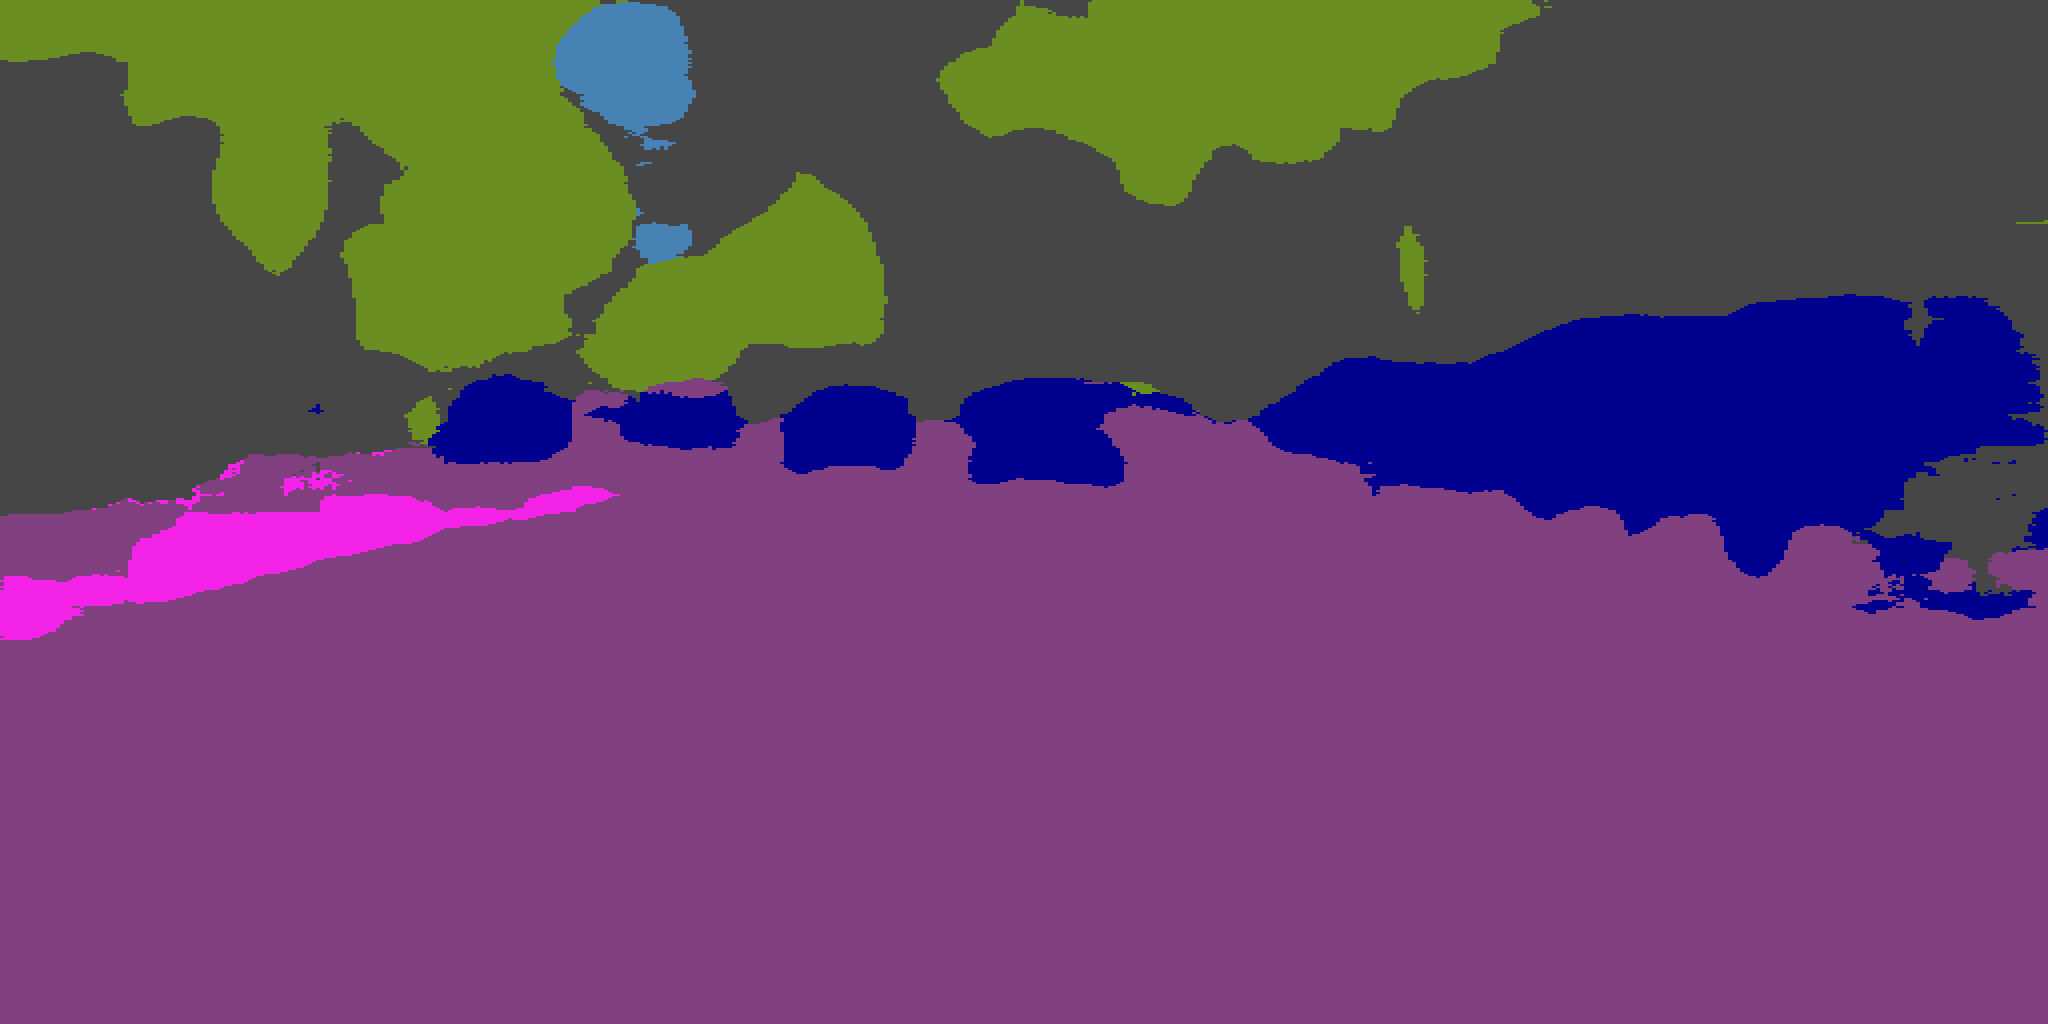
\includegraphics[width=0.8\linewidth]{Images/frankfurt_000000_015676_5_leftImg8bit}
  \caption{\textgreek{Πρόβλεψη μοντέλου }SD-CNN \textgreek{χωρίς ισοστάθμιση κλάσεων}.}
  \end{subfigure}
 ~
 \begin{subfigure}[b]{\linewidth}
 \centering
 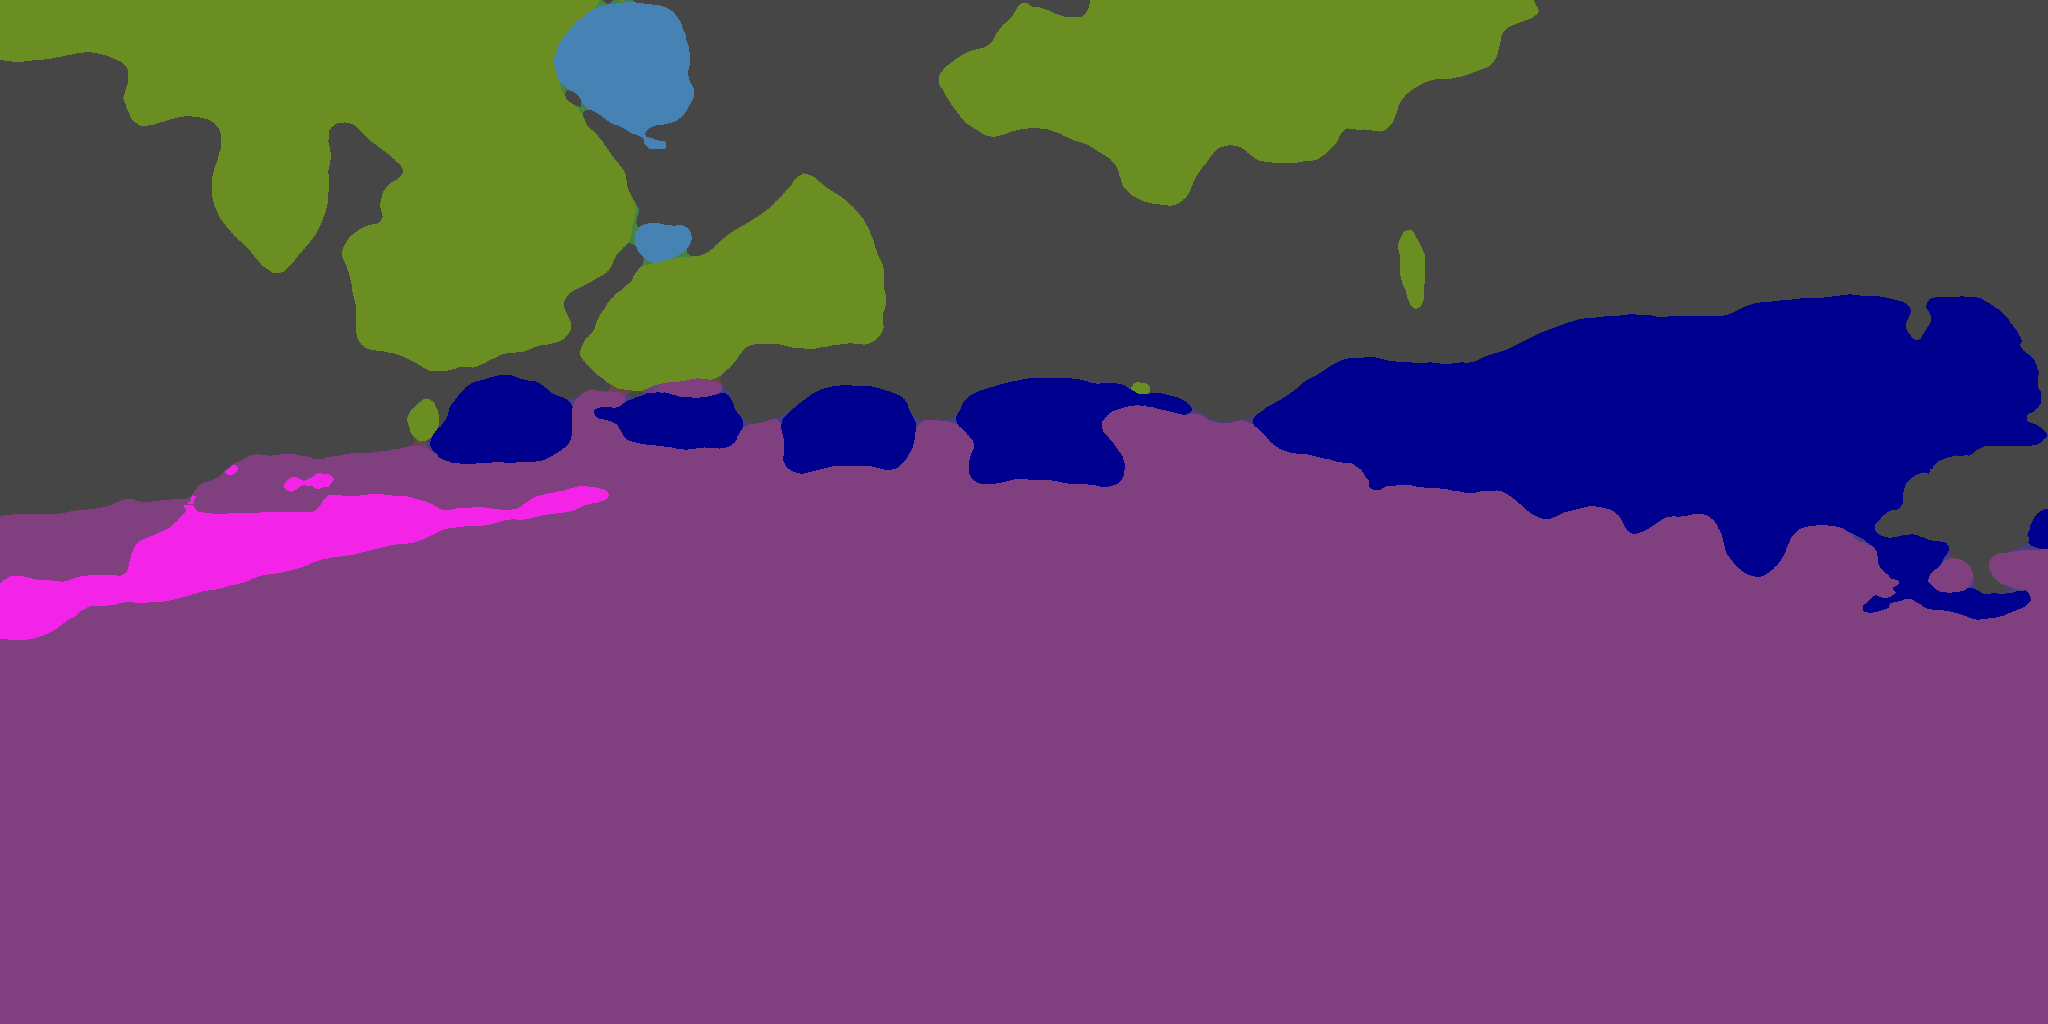
\includegraphics[width=0.8\linewidth]{Images/frankfurt_000000_015676_5_median_leftImg8bit}
  \caption{\textgreek{Πρόβλεψη μοντέλου }SD-CNN \textgreek{χωρίς ισοστάθμιση κλάσεων με την εφαρμογή του βέλτιστου παραθύρου μεσαίου φίλτρου}.}
  \end{subfigure}
  ~
  \begin{subfigure}[b]{\linewidth}
  \centering
  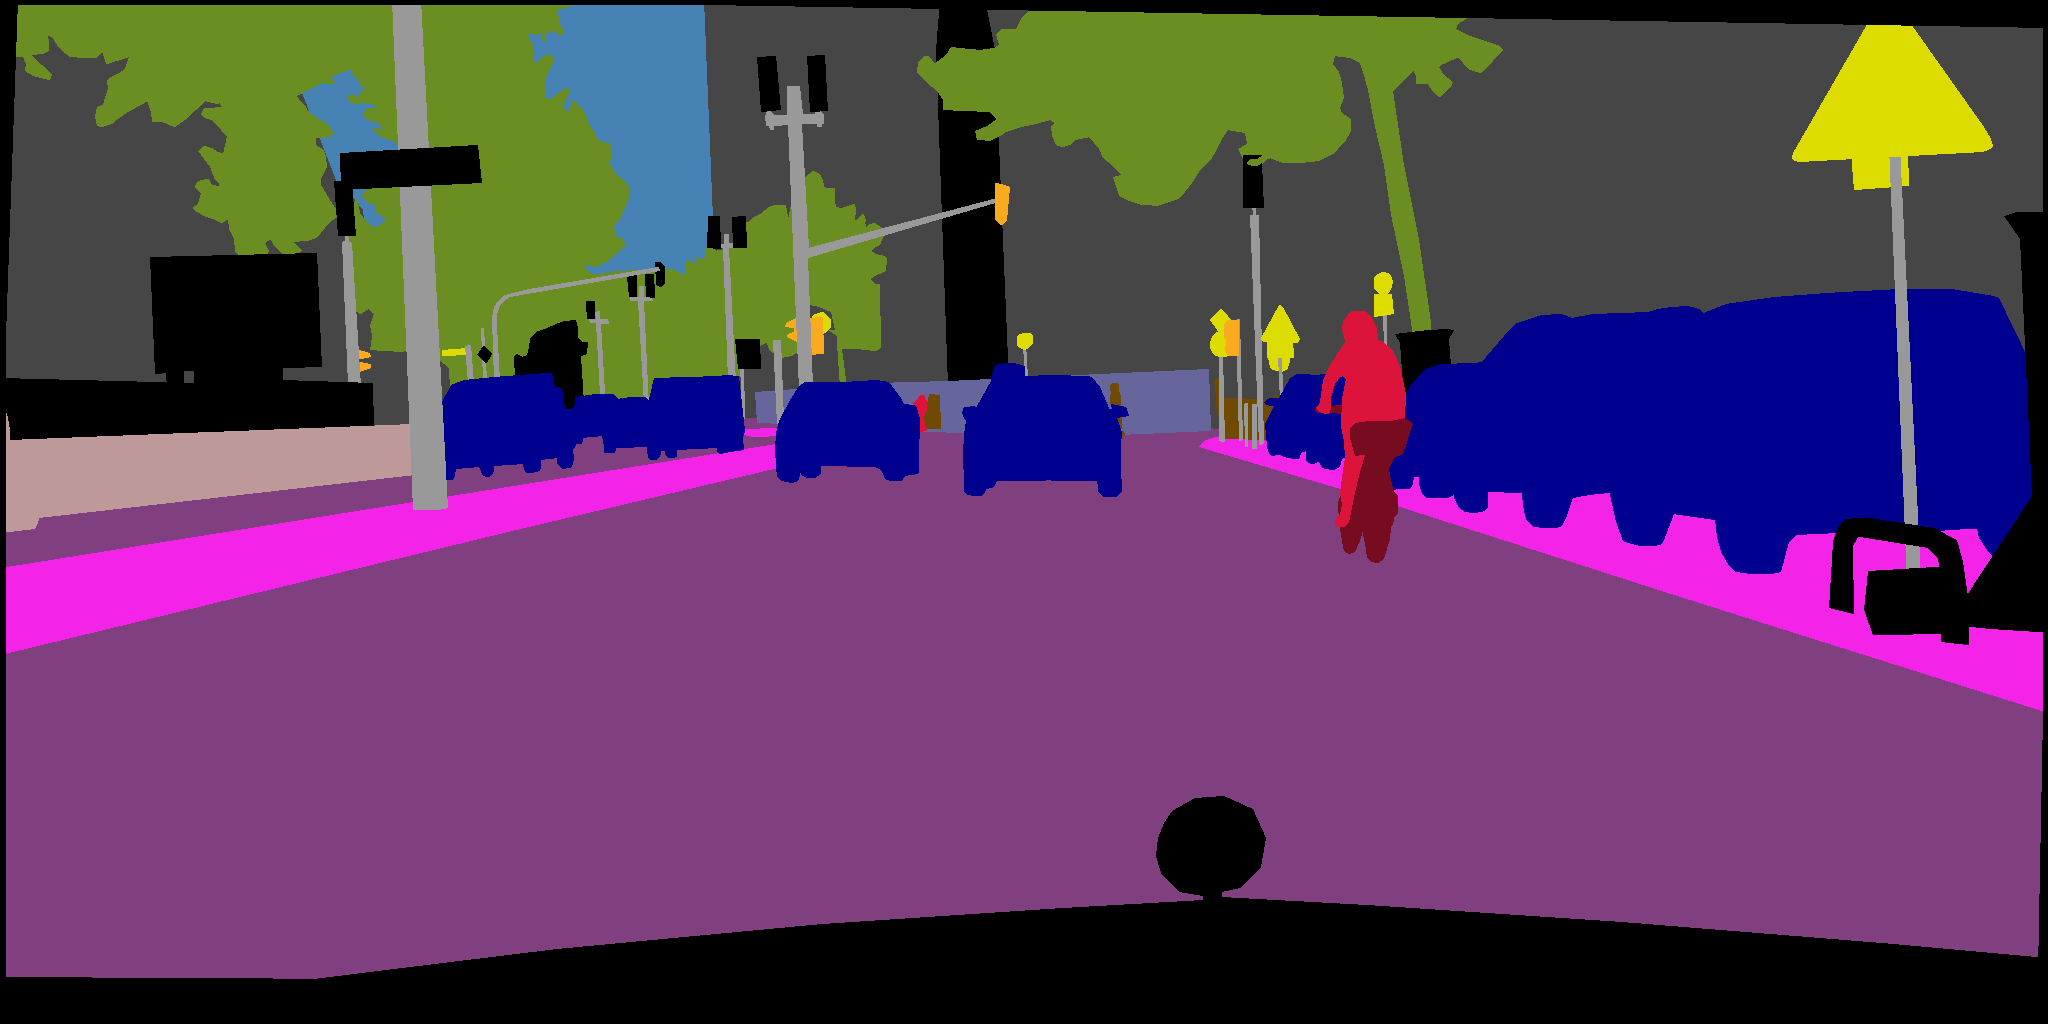
\includegraphics[width=0.8\linewidth]{Images/frankfurt_000000_015676_gtFine_color}
  \caption{Ground Truth}
 \end{subfigure}
  \caption[\textgreek{Εικόνες από ΠΣΝΔ}]{\textgreek{Εικόνες αποτελεσμάτων του ΠΣΝΔ χωρίς ισοστάθμιση κλάσεων με εφαρμογή μεσαίου φίλτρου και χωρίς.}}
 \label{fig:image_results_2}
\end{figure}

%%%%
\begin{figure}[H]
 \centering
 \begin{subfigure}[b]{\linewidth}
 \centering
 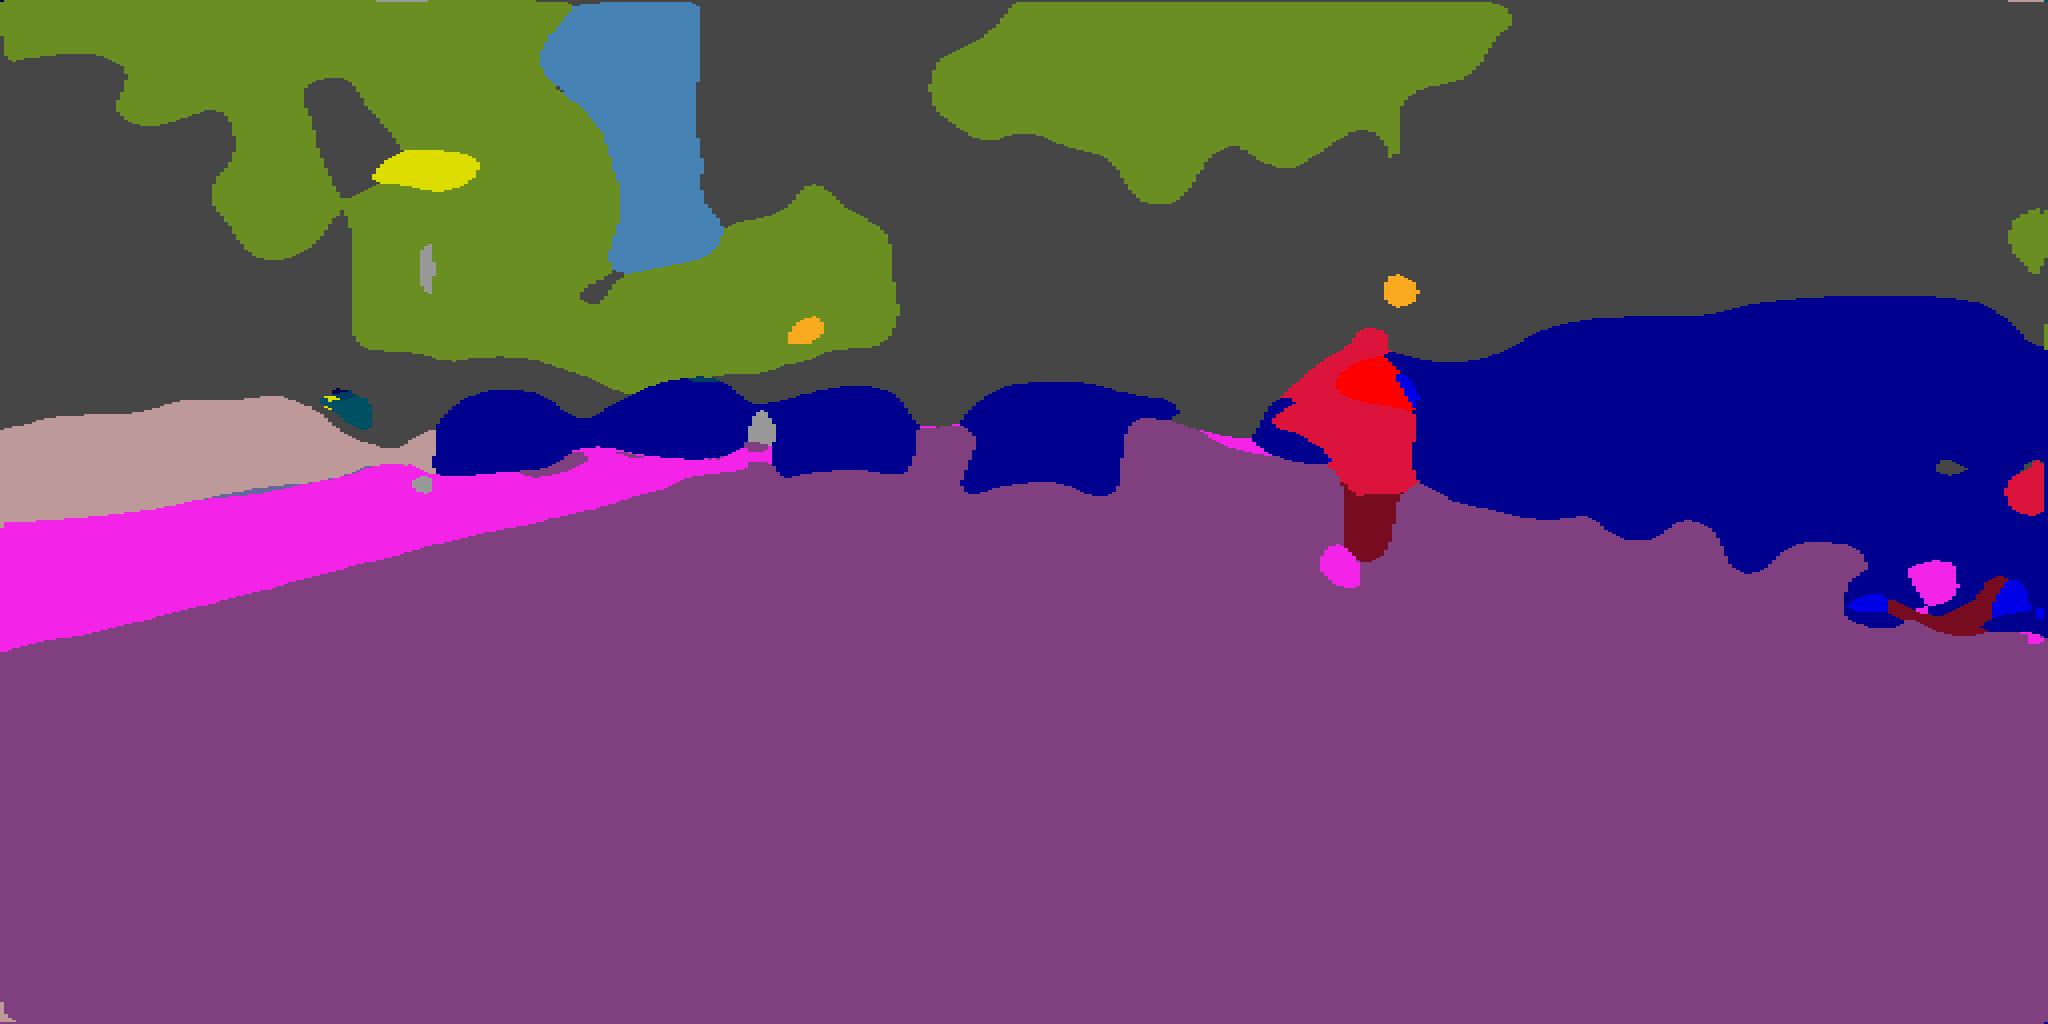
\includegraphics[width=0.8\linewidth]{Images/image_predictions_HighREs_512_11}
  \caption{\textgreek{Πρόβλεψη μοντέλου }BD-CNN \textgreek{χωρίς εφαρμογή φίλτρου}.}
  \end{subfigure}
 ~
 \begin{subfigure}[b]{\linewidth}
 \centering
 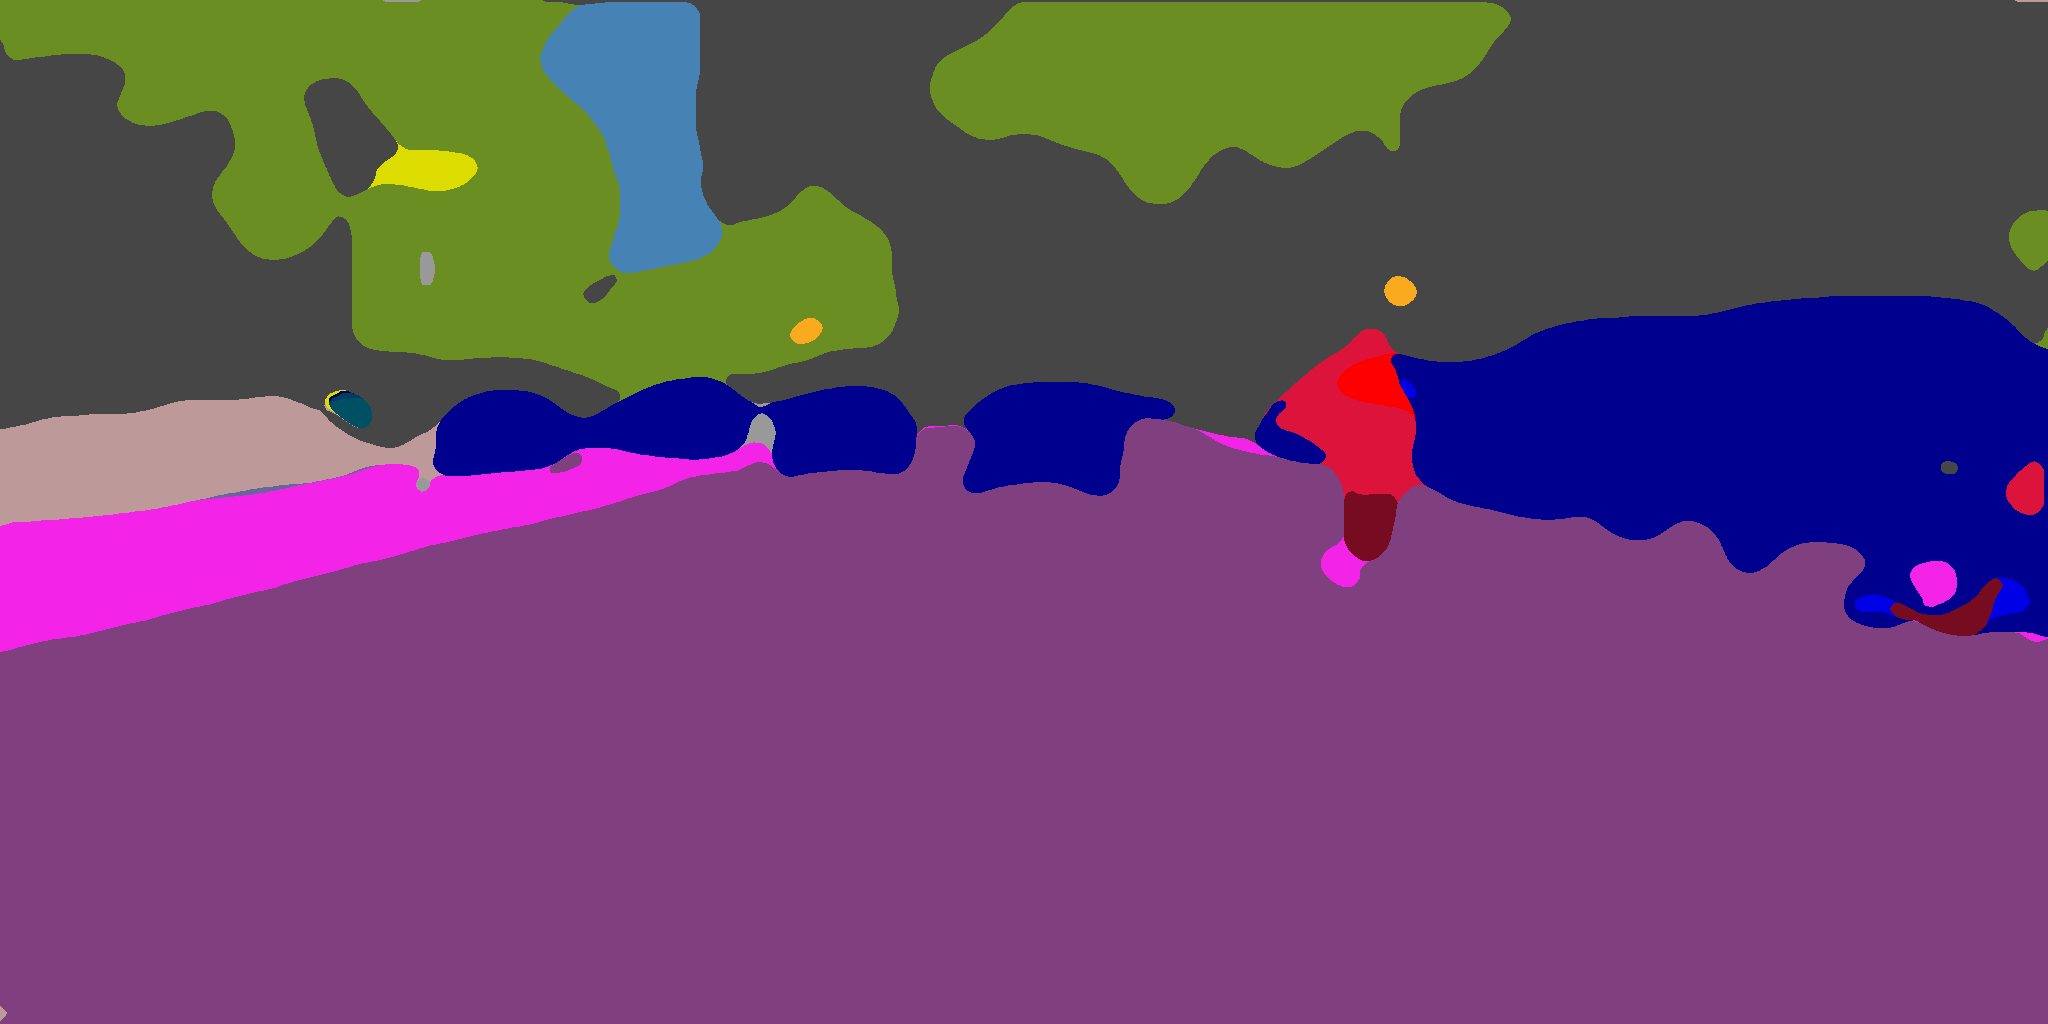
\includegraphics[width=0.8\linewidth]{Images/image_predictions_HighREs_median_512_11}
  \caption{\textgreek{Πρόβλεψη μοντέλου }BD-CNN \textgreek{με την εφαρμογή του βέλτιστου παραθύρου ($19\times 19$) του μεσαίου φίλτρου}.}
  \end{subfigure}
  ~
  \begin{subfigure}[b]{\linewidth}
  \centering
  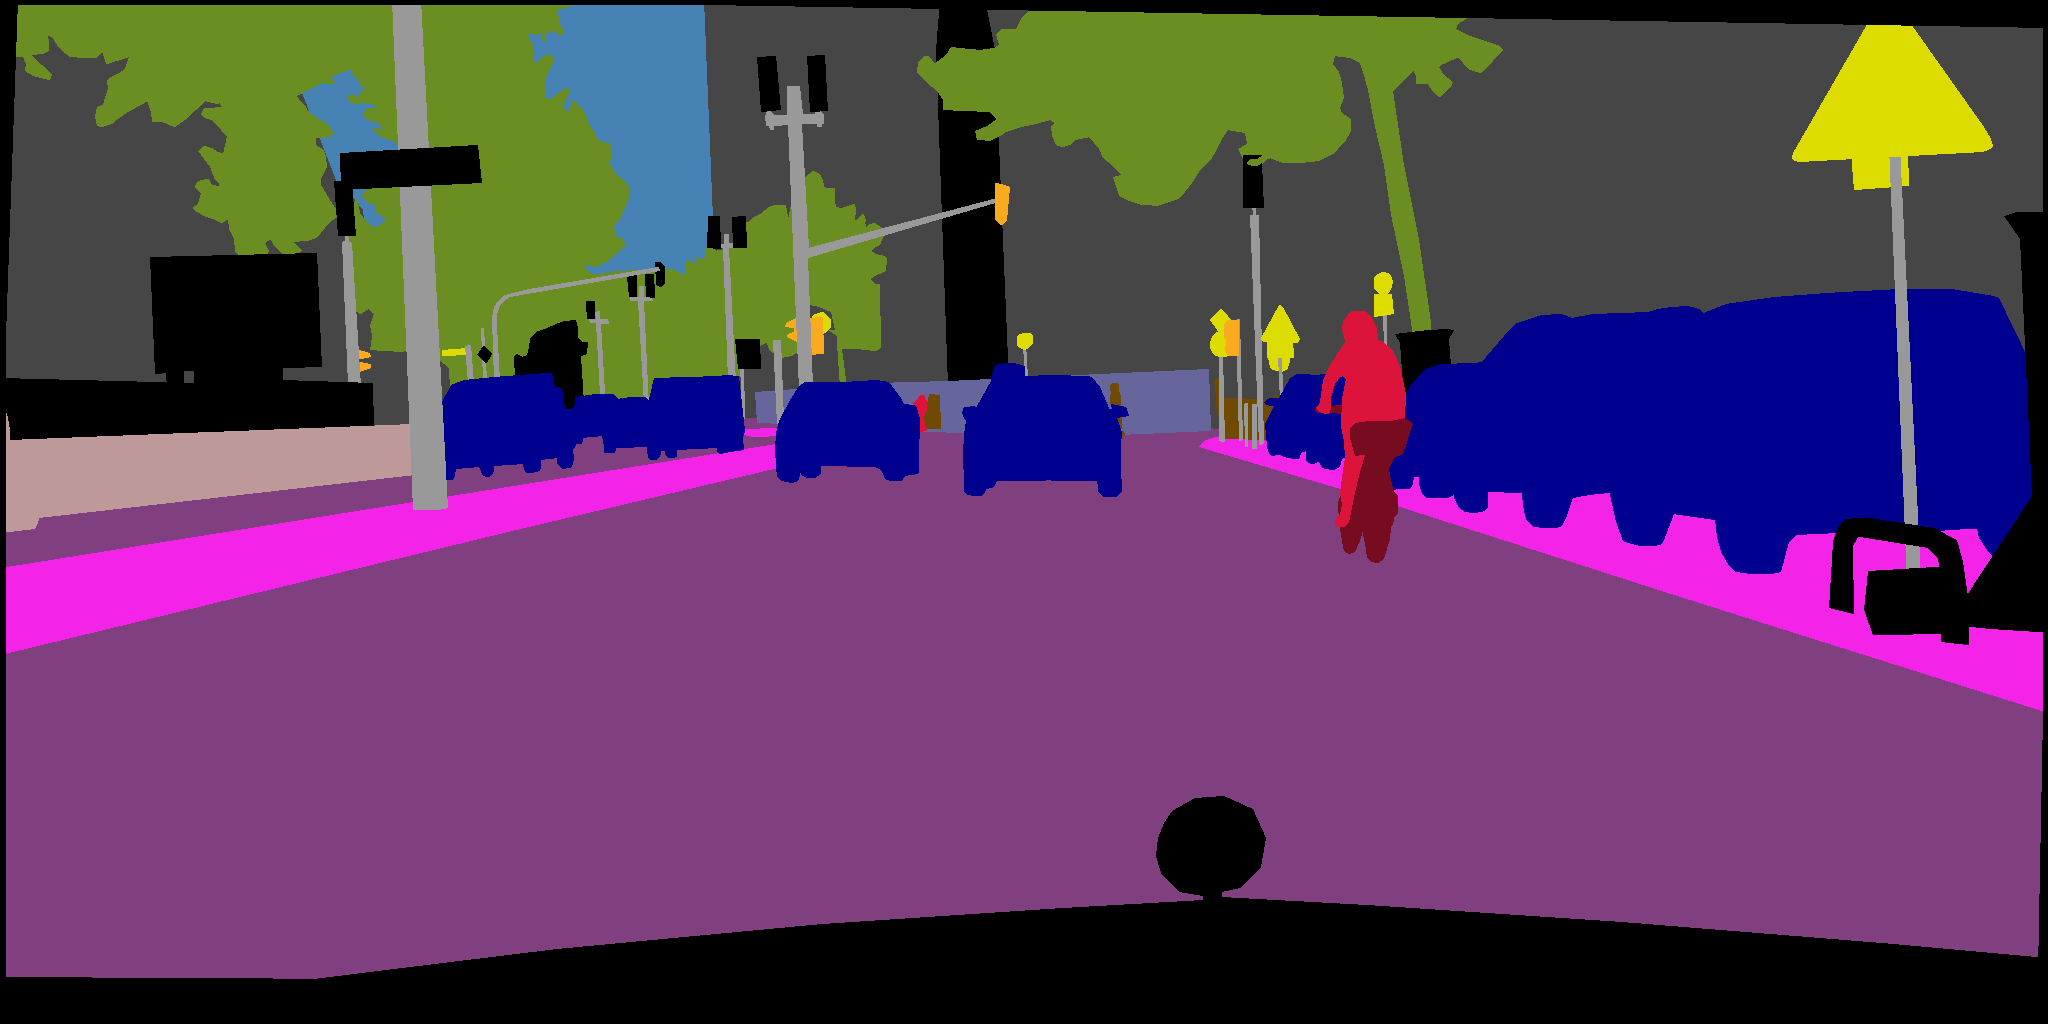
\includegraphics[width=0.8\linewidth]{Images/frankfurt_000000_015676_gtFine_color}
  \caption{Ground Truth}
 \end{subfigure}
  \caption[\textgreek{Εικόνες Διγραμμικών ΠΣΝΔ}]{\textgreek{Εικόνες αποτελεσμάτων του ΠΣΝΔ χωρίς ισοστάθμιση κλάσεων με εφαρμογή μεσαίου φίλτρου και χωρίς.}}
 \label{fig:image_results_3}
\end{figure}

\pagebreak
\textgreek{Οι πίνακες σύγχυσης που βλέπουμε παρακάτω στις εικόνες αποτελούν μια πιο αξιόπιστη μέθοδο οπτικοποίησης των αποτελεσμάτων για να δούμε πόσο ισχυρά είναι τα μοντέλα μας και ποιες κατηγορίες μπερδεύονται περισσότερο μεταξύ τους. Οι πίνακες παρουσιάζονται με μια κανονικοποιημένη μορφή, ενώ όσο πιο έντονο είναι το χρώμα στην διαγώνιο του πίνακα τόσο πιο δυνατό είναι το μοντέλο. Η μετρική }Jaccard Similarity \textgreek{που είδαμε προηγουμένως επειδή υπολογίζει καθολικά σε όλη την εικόνα τις παραμέτρους της και βγάζει μια μέση τιμή από αυτές δεν δύναται να μας δώσει σωστά την ακρίβεια για κάθε κατηγορία. Στην αριστερή πλευρά των πινάκων σύγχυσης έχουμε τις πραγματικές κατηγοριοποιήσεις των εικονοστοιχείων ενώ κάθετα έχουμε τις προβλέψεις των μοντέλων μας. Η τελευταία στήλη και σειρά ανήκουν στην κατηγορία 'χωρίς ετικέτα' για αυτό και το αφήσαμε κενό. \par  }

\textgreek{Η εικόνα }\ref{fig:cf_1} \textgreek{μας συγκρίνει τα μοντέλα που δεν έχουν εκπαιδευτεί με την μέθοδο της ισοστάθμισης. Για τους λόγους που εξηγήσαμε προηγουμένως, το μοντέλο με την διγραμμική μονάδα (εικόνα }\ref{fig:image_results_3}) \textgreek{τα πηγαίνει αρκετά καλύτερα.}

\textgreek{Τέλος, στην εικόνα }\ref{fig:cf_2} \textgreek{επιδεικνύεται η σύγκριση μεταξύ του μοντέλου }SD-CNN \textgreek{με ισοστάθμιση των κλάσεων (εικόνα} \ref{fig:image_results_2}) \textgreek{καθώς και του }end-to-end \textgreek{μοντέλου }SD-CNN-CRF-RNN \textgreek{ με αριθμό επαναλήψεων επανεκτίμησης ίσο με πέντε. Η διαφορά μεταξύ των δύο μοντέλων δεν είναι πολύ μεγάλη άλλωστε όπως είδαμε και πριν ήταν μόλις 1\%. Όμως μπορούμε να δούμε πως πολλές λανθασμένες προβλέψεις έχουν μειωθεί αρκετά και αυτό δείχνει την ισχύ του μοντέλου μετα-επεξεργασίας. Αξίζει να δούμε την κλάση μοτοσυκλέτα η οποία έχει μειωθεί στο ΤΥΣΠ-ΕΝΔ. Πιθανόν τα εικονοστοιχεία που ταιριάζουν σε αυτή την κλάση, μοιάζουν αρκετά με εικονοστοιχεία κάποιας άλλης κλάσης και για αυτό τυχαίνει να υπάρχει μείωση. Οι πίνακες σύγχυσης υπολογίστηκαν πάνω στις 500 εικόνες του συνόλου δεδομένων επαλήθευσης στο αρχικό μέγεθος της εικόνας.} 

%%%% CONFUSION MATRICES
\newpage
\begin{figure}[H]
\centering
\begin{subfigure}[b]{\linewidth}
 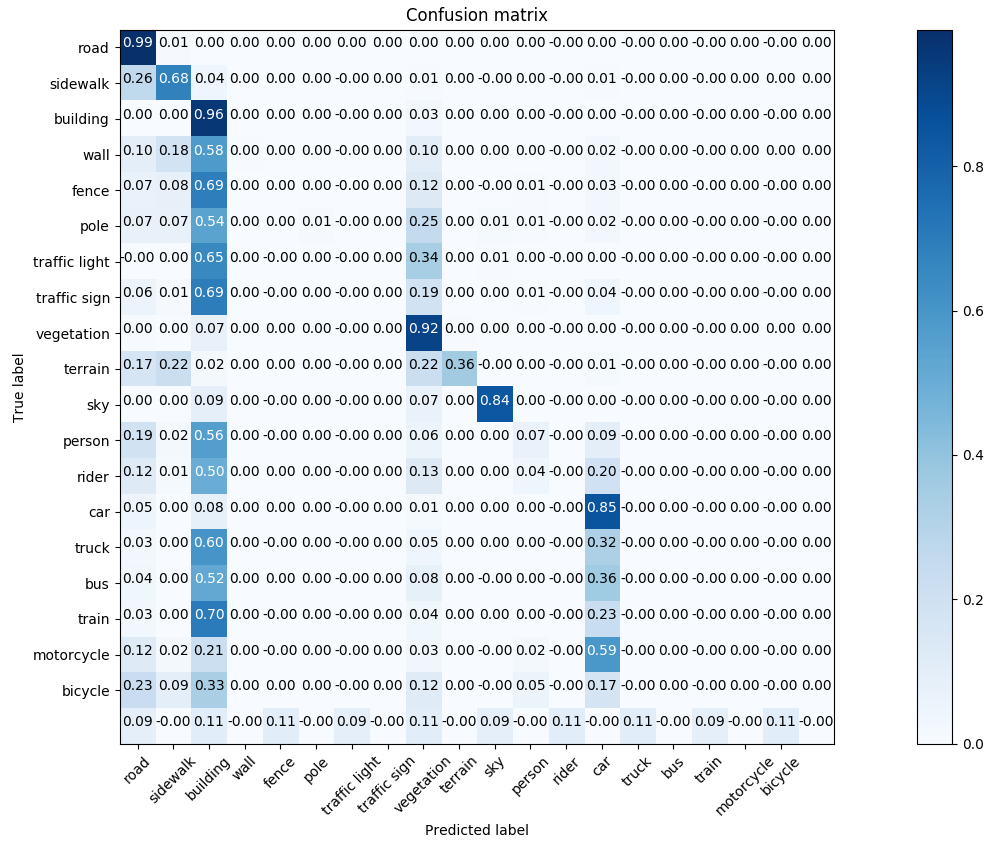
\includegraphics[scale=0.38 ]{Images/final_CF_5}
 \caption{\textgreek{Πίνακας Σύγχυσης του ΠΣΝΔ με μονάδα αποκωδικοποίησης με άλμα ολίσθησης} (SD-CNN)\textgreek{ χωρίς εφαρμογή της συνάρτησης ισοστάθμισης.}}
\end{subfigure}
\\[1pt]
\begin{subfigure}[b]{\linewidth}
 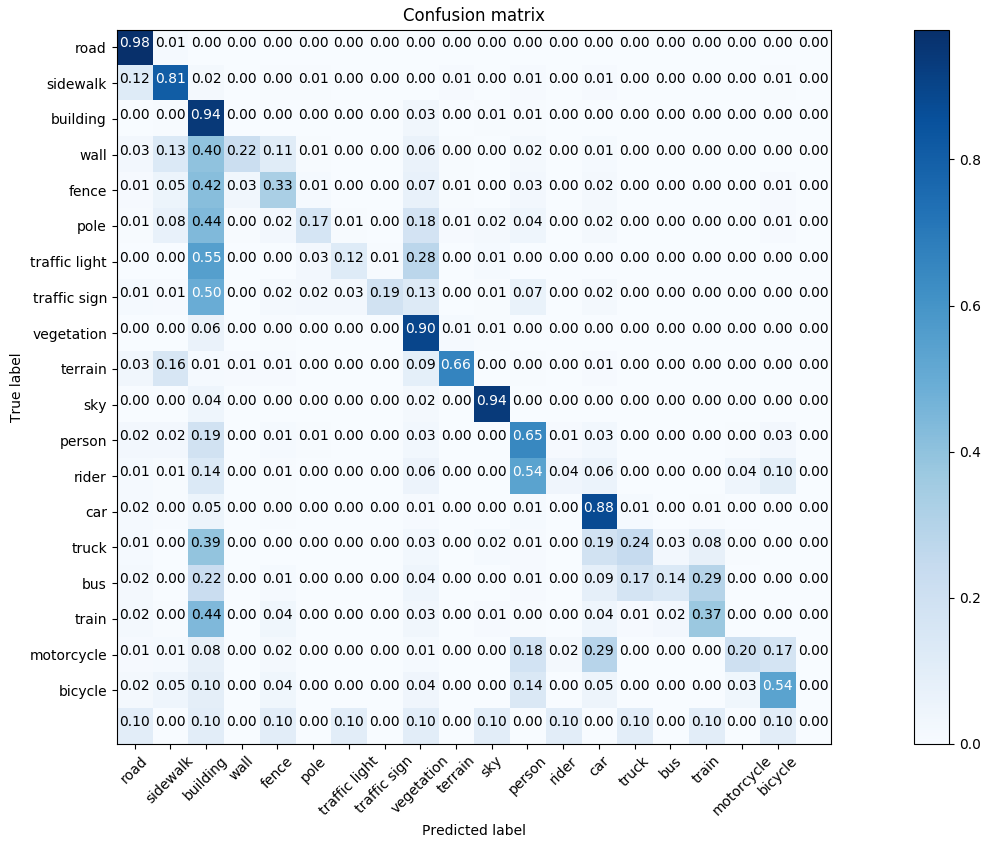
\includegraphics[scale=0.38]{Images/final_CF_11}
 \caption{\textgreek{Πίνακας Σύγχυσης του ΠΣΝΔ με διγραμμική μονάδα αποκωδικοποίησης} (BD-CNN)\textgreek{ χωρίς εφαρμογή της συνάρτησης ισοστάθμισης.}}
 \end{subfigure}
 
\caption[\textgreek{Πίνακες Σύγχυσης χωρίς μετα-επεξεργασία}]{\textgreek{Πίνακες σύγχυσης των μοντέλων χωρίς μονάδες μετα-επεξεργασίας και ισοστάθμιση των κλάσεων.}}
\label{fig:cf_1}
\end{figure}


\begin{figure}[H]
\centering
\begin{subfigure}[b]{1\linewidth}
 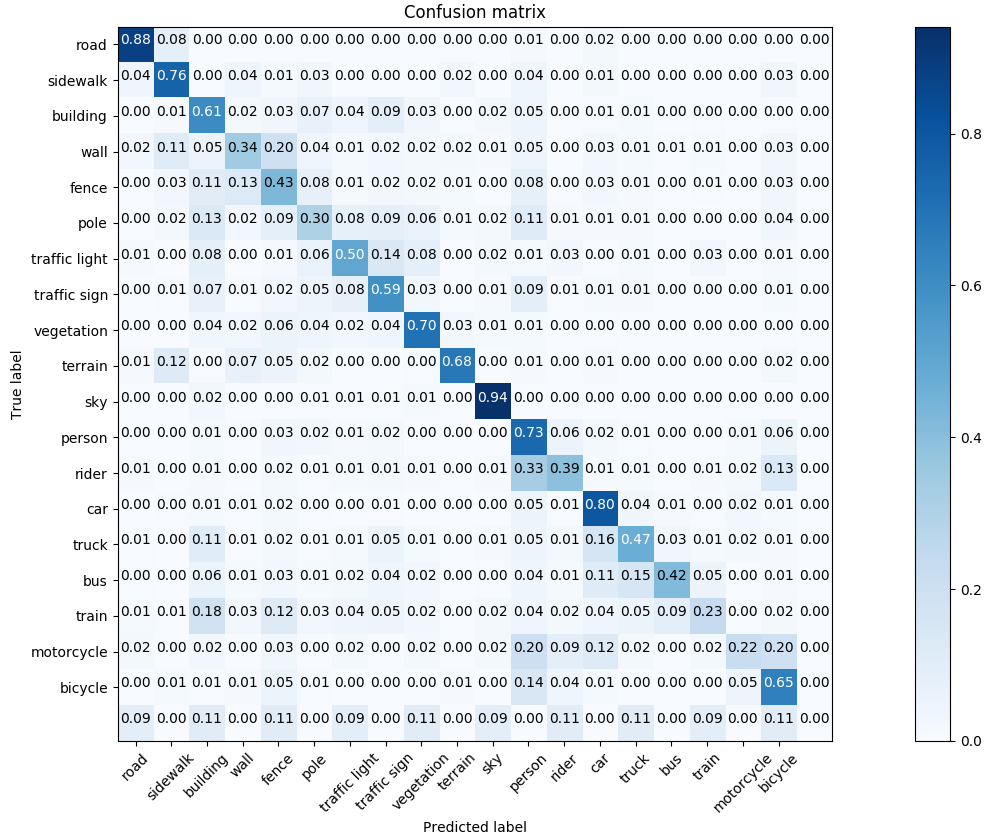
\includegraphics[scale=0.36]{Images/final_CF_7} \\[1pt]
 \caption{\textgreek{Πίνακας Σύγχυσης του ΠΣΝΔ με μονάδα αποκωδικοποίησης με άλμα ολίσθησης} (SD-CNN)\textgreek{ με ισοστάθμιση των κλάσεων.}}
 \end{subfigure}
\begin{subfigure}[b]{1\linewidth}
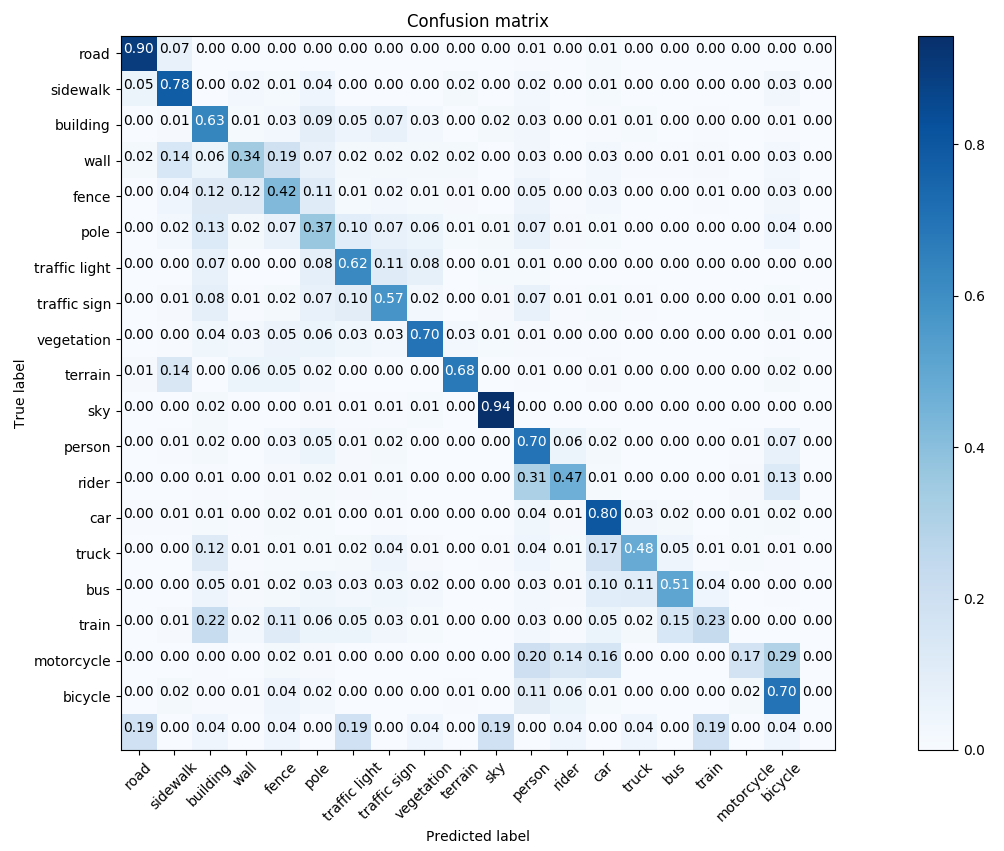
\includegraphics[scale=0.36]{Images/final_CF_7_CRF5}
\caption{\textgreek{Πίνακας Σύγχυσης του ΠΣΝΔ με μονάδα αποκωδικοποίησης με άλμα ολίσθησης και με μονάδα μετα-επεξεργασίας ΤΥΣΠ-ΕΝΔ} (SD-CNN-CRF)\textgreek{ με ισοστάθμιση των κλάσεων.}}
\end{subfigure}
\caption[\textgreek{Πίνακες Σύγχυσης με ΤΥΣΠ-ΕΝΔ}]{\textgreek{Πίνακες σύγχυσης για την σύγκριση των μοντέλων με και χωρίς μονάδα μετα-επεξεργασίας και ισοστάθμιση των κλάσεων.}}\label{fig:cf_2}
\end{figure}

\chapter{\textgreek{Συμπεράσματα και Μελλοντική Εργασία}}

\pagestyle{fancy}
\fancyhf{}
%\fancyhead[OC]{\leftmark}
%\fancyhead[C]{}
%\fancyhead[EC]{\rightmark}
\renewcommand{\footrulewidth}{0.5pt}
\cfoot{\thepage}

\section{\textgreek{Συμπεράσματα}}
\textgreek{Ο σκοπός της συγκεκριμένης διπλωματικής ήταν η εξερεύνηση και η σύγκριση τεχνικών τελευταίας γενιάς στο πεδίο της μηχανικής μάθησης για το πρόβλημα της σημασιολογικής κατάτμησης αντικειμένων από εικόνες αλλά και η δημιουργία κατάλληλου εργαλείου για την προβολή των προβλέψεων από τα μοντέλα. Πιο συγκεκριμένα, επικεντρωθήκαμε στην εφαρμογή μεθόδων βαθιάς μάθησης με χρήση αρχιτεκτονικών ΠΣΝΔ με το μοντέλο γράφων ΤΥΣΠ-ΕΝΔ για την εκτίμηση της κατηγορίας που ανήκει κάθε εικονοστοιχείο της εικόνας. Τα δίκτυα ΠΣΝΔ αποτελούν μια από τις τεχνικές τελευταίας γενιάς στα προβλήματα σημασιολογικής κατάτμησης ειδικά σε συνδυασμό με τους γράφους ΤΥΣΠ καθώς έχουν επιδείξει πολύ καλά αποτελέσματα. 
\par
Μια ενδιαφέρουσα συνεισφορά της εργασίας είναι η χρήση της εκθετικής συνάρτησης ενεργοποίησης η οποία σε συνδυασμό με την σωστή συνάρτηση αρχικοποίησης των βαρών αντιμετωπίζουν το πρόβλημα των νεκρών νευρώνων το οποίο τείνουν να πάσχουν τα βαθειά ΝΔ. Επίσης, αυτή η προσέγγιση είναι πιο αποδοτική καθώς δεν προσθέτει υπολογιστικό κόστος στην εκπαίδευση του ΝΔ σε σχέση με άλλες προσεγγίσεις.
\par
Τέλος, παρουσιάσαμε και συγκρίναμε δύο πανομοιότυπες αρχιτεκτονικές βασισμένες σε ΣΝΔ κωδικοποίησης και αποκωδικοποίησης και πως αυτές ανταποκρίνονται. Είναι φανερό πως το ΣΝΔ με την μονάδα αποκωδικοποίησης με άλμα ολίσθησης αν και διαθέτει μεγαλύτερο αριθμό παραμέτρων, δίνει καλύτερα αποτελέσματα λόγω της μη γραμμικής υπερδειγματοληψίας η οποία διαθέτει παραμέτρους που μαθαίνουν την χαρτογράφηση της υπερδειγματοληψίας κατά την εκπαίδευση.  Επίσης, η χρησιμότητα της συνάρτησης μέσης συχνότητας ισορροπίας, η οποία παίζει σημαντικό ρόλο σε τέτοιου είδος προβλήματα στο στάδιο της εκπαίδευσης, καθώς επιτυγχάνεται μια ισορροπία ως ένα βαθμό μεταξύ της δυσαναλογίας των κλάσεων που υπάρχει στα δεδομένα. 
}
\newpage
\section{\textgreek{Μελλοντική Εργασία}}
\textgreek{Το θέμα της σημασιολογικής κατάτμησης κεντρίζει όλο και περισσότερο το ενδιαφέρον των επιστημόνων καθώς αποτελεί πρόκληση στον κλάδο, ενώ η συνεχής ανάπτυξη της υπολογιστικής δύναμης η οποία είναι απαραίτητη σε συνδυασμό με την δημιουργία καινούριων αυτόνομων μηχανών που παίρνουν αποφάσεις σύμφωνα με τον ακριβή διαχωρισμό των αντικειμένων στο περιβάλλον} \cite{deepNAT, Home3d}, \textgreek{έχουν σαν αποτέλεσμα την μεταστροφή από προβλήματα ανίχνευσης αντικειμένων στην σημασιολογική κατάτμηση.
\par
Στο μέλλον θα θέλαμε να χρησιμοποιήσουμε πιο βαθειά μοντέλα χρησιμοποιώντας λιγότερη υποδειγματοληψία στις εικόνες εισόδου για περισσότερη πληροφορία. Επίσης θα θέλαμε να χρησιμοποιήσουμε περισσότερα δεδομένα, όμως υπάρχει δυσκολία σε αυτό το κομμάτι καθώς θα πρέπει να δημιουργηθούν καινούριες εικόνες με κατηγοριοποιημένα όλα τα εικονοστοιχεία. Μία καλή προσέγγιση θα ήταν η δημιουργία συνθετικών δεδομένων από τις ήδη υπάρχουσες εικόνες. Οι συνθετικές εικόνες δημιουργούνται με εφαρμογή από μια πληθώρα κατάλληλων φίλτρων πάνω στις εικόνες ώστε να δημιουργήσουμε παραλλαγές των εικόνων και ως αποτέλεσμα περισσότερα δεδομένα για την αντιμετώπιση του προβλήματος της υπερμάθησης. Επίσης, θα θέλαμε να δοκιμάσουμε την αρχιτεκτονική με την διγραμμική υπερδειγματοληψία με περισσότερα φίλτρα σε συνδυασμό με την μονάδα ΤΥΣΠ-ΕΝΔ καθώς είναι πιθανόν να υπάρχουν προοπτικές. 
}
\par
\textgreek{Μία διαφορετική κατεύθυνση είναι η χρήση ενός προ-εκπαιδευμένου ΠΣΝΔ το οποίο έχει εκπαιδευτεί σε κάποιο διαφορετικό πρόβλημα. Η χρήση ενός τέτοιου μοντέλου βοηθάει στην εξαγωγή πολύπλοκων χαρακτηριστικών τα οποία μπορούν να τροφοδοτήσουν ένα ΠΣΝΔ όπως το δικό μας. Η εκπαίδευση ενός τέτοιου μοντέλου σε συνδυασμό με το δικό μας μοντέλο θα μπορούσε να προσφέρει καλύτερα αποτελέσματα. Ο μεγαλύτερος αριθμός παρτίδας επίσης, θα μπορούσε να επιφέρει καλύτερα αποτελέσματα, καθώς χρησιμοποιήσαμε μία παρτίδα της τάξης του 4 στην καλύτερη περίπτωση, ο υπολογισμός σε περισσότερα δεδομένα σε κάθε επανάληψη και ανανέωση των κρυμμένων στοιχείων ανά περισσότερα κομμάτια θα μπορούσε να βελτιώσει τα αποτελέσματα. Δυστυχώς, η αύξηση της παρτίδας και ειδικά σε δεδομένα πολύ μεγάλων διαστάσεων απαιτούν και αρκετούς πόρους.
\par 
Τέλος, η παράλληλη μονάδα επεξεργασίας θα μπορούσε να βελτιώσει τα αποτελέσματα αν μπορούσαμε να την χρησιμοποιήσουμε με μεγαλύτερα μεγέθη χαρτών χαρακτηριστικών στην είσοδο, καθώς θα μπορούσαν να αποδώσουν καλύτερα στην αξιοποίηση της πληροφορίας λόγω της μικρότερης συμπίεσης. Επίσης η αύξηση των αριθμών των φίλτρων σε κάθε κλάδο θα μπορούσαν να αποδώσουν θετικά καθώς θα υπήρχαν περισσότεροι χάρτες χαρακτηριστικών, όμως αυτή η επιλογή έρχεται με αντάλλαγμα την αύξηση των παραμέτρων.}



% Appendix Chapter
\chapter*{\textgreek{Παράρτημα Α}}

\pagestyle{fancy}
\fancyhf{}
%\fancyhead[OC]{\leftmark}
\fancyhead[C]{}
%\fancyhead[EC]{\rightmark}
\renewcommand{\footrulewidth}{1pt}
\cfoot{\thepage}

\textgreek{Οι αλγόριθμοι και τα μοντέλα που χρησιμοποιήθηκαν σε αυτή την διπλωματική βρίσκονται στο προφίλ του συγγραφέα στο }Github \textgreek{στον παρακάτω σύνδεσμο} \href{https://github.com/dimimal/semantics_segmentation_of_urban_environments}{link}. \textgreek{Σε αυτό το τμήμα θα δείξουμε το λογισμικό το οποίο υλοποιήθηκε στα πλαίσια της εργασίας για την οπτικοποίηση των αποτελεσμάτων. Το λογισμικό υλοποιήθηκε με την χρήση των βιβλιοθηκών }pyQt4 \cite{pyqt_doc} \textgreek{και} OpenCV \cite{opencv_lib,opencv_man}, \textgreek{ενώ για την υλοποίηση των μοντέλων χρησιμοποιήθηκαν οι βιβλιοθήκες } Keras \cite{keras_bib}, Tensorflow \cite{tensorflow_bib} \textgreek{και} scikit-learn \cite{sklearn_bib}.
\par

\textgreek{Ο πίνακας }\ref{tb:class_colors} \textgreek{επιδεικνύει τα χρώματα που αντιστοιχούν στην κάθε κλάση τα οποία χρησιμοποιούνται στο λογισμικό για την οπτικοποίηση των κλάσεων. Κάθε εικονοστοιχείο το οποίο ανήκει σε κάποια συγκεκριμένη κλάση αντιστοιχεί και το αντίστοιχο χρώμα. }


\begin{table}[H]

\begin{tabular}{|l|l|l|l|l|}
\hline
 \cellcolor[HTML]{804080}\textgreek{Δρόμος} & \cellcolor[HTML]{F423E8}\textgreek{Πεζοδρόμιο} & \cellcolor[HTML]{464646}\textgreek{Κτίριο} & \cellcolor[HTML]{66669C}\textgreek{Τοίχος}& \cellcolor[HTML]{BE9999}\textgreek{Φράχτης}\\ \hline    

\cellcolor[HTML]{999999}\textgreek{Ιστός} & \cellcolor[HTML]{FAAA1E}\textgreek{Φανάρι Κυκλοφορίας} & \cellcolor[HTML]{DCDC00}\textgreek{Πινακίδα Κυκλοφορίας} & \cellcolor[HTML]{6B8E23}\textgreek{Βλάστηση}& \cellcolor[HTML]{98FB98}\textgreek{Έδαφος}\\ 

\cellcolor[HTML]{4682B4}\textgreek{Ουρανός} & \cellcolor[HTML]{DC143C}\textgreek{Άνθρωπος} & \cellcolor[HTML]{FF0000}\textgreek{Αναβάτης} & \cellcolor[HTML]{00008E}\textcolor{white}{\textgreek{Αυτοκίνητο}} & \cellcolor[HTML]{000046} \textcolor{white}{\textgreek{Φορτηγό}} \\

\cellcolor[HTML]{003C64}\textgreek{Λεωφορείο} & \cellcolor[HTML]{005064}\textgreek{Τρένο} & \cellcolor[HTML]{0000E6}\textcolor{white}{\textgreek{Μοτοσυκλέτα}} & \cellcolor[HTML]{770B20}\textgreek{Ποδήλατο} & \cellcolor[HTML]{000000}\textcolor{white}{\textgreek{Κενό}} \\ \hline

\end{tabular}
\caption[\textgreek{Πίνακας Χρωμάτων των Κλάσεων}]{\textgreek{Χρώματα των διαφορετικών αντικειμένων τα οποία φαίνονται στο παρακάτω λογισμικό. }}\label{tb:class_colors}
\end{table}





\textgreek{Το λογισμικό που θα δούμε παρακάτω βασίστηκε στο λογισμικό που έχει δημιουργηθεί από την ομάδα της βάσης δεδομένων }Cityscapes \cite{Cityscapes}.\textgreek{Όπως βλέπουμε στις εικόνες} \ref{fig:viewer_1}, \ref{fig:viewer_2} \textgreek{κατά την εκτέλεση του  προγράμματος εμφανίζεται παράθυρο επιλογής μίας εικόνας για αναγνώριση και ακολουθεί δεύτερο παράθυρο αντίστοιχα για την επιλογή ενός αρχείου/εικόνας το οποίο περιέχει τις προβλέψεις που έχουν παραχθεί από το μοντέλο μας. }
\begin{figure}[H]
 \centering
 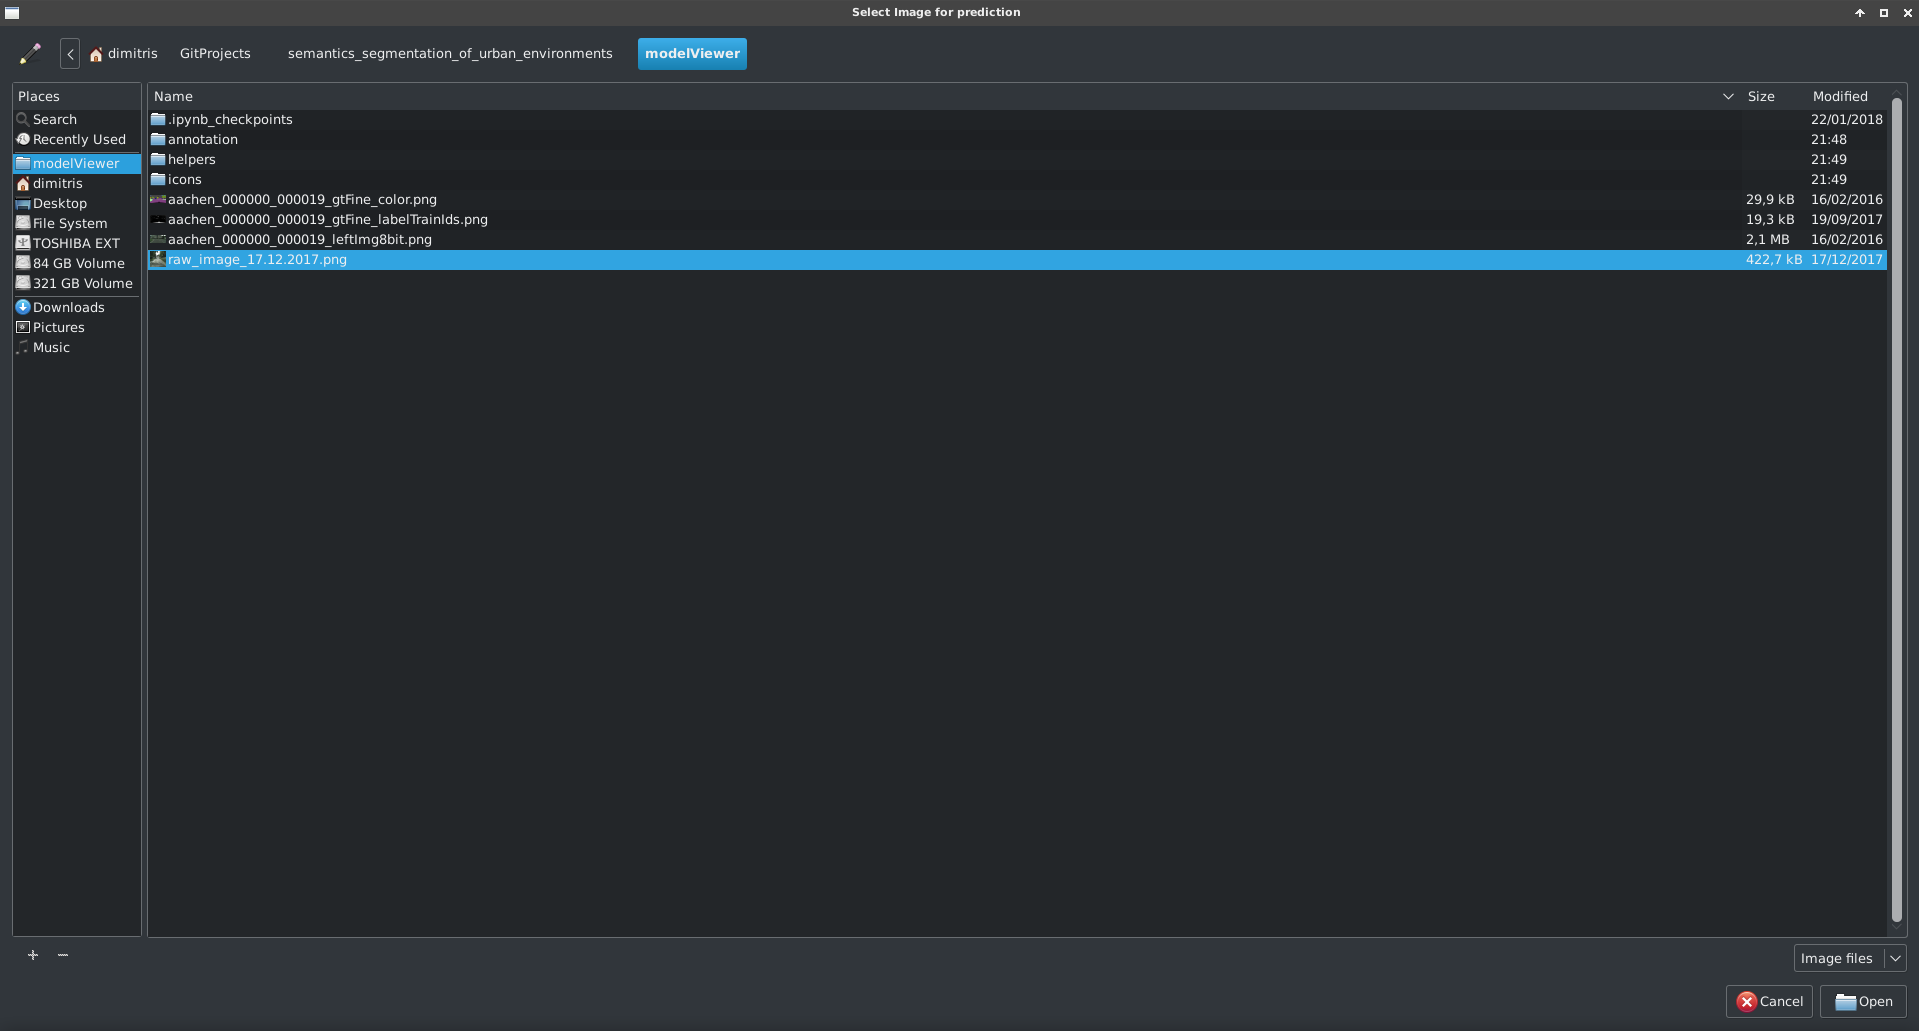
\includegraphics[width=\textwidth, scale=0.3]{Images/viewer_1}
\caption[\textgreek{Επιλογή Εικόνας}]{\textgreek{Επιλογή αρχικής εικόνας για αναγνώριση.}}\label{fig:viewer_1}
\end{figure}

\begin{figure}[H]
 \centering
 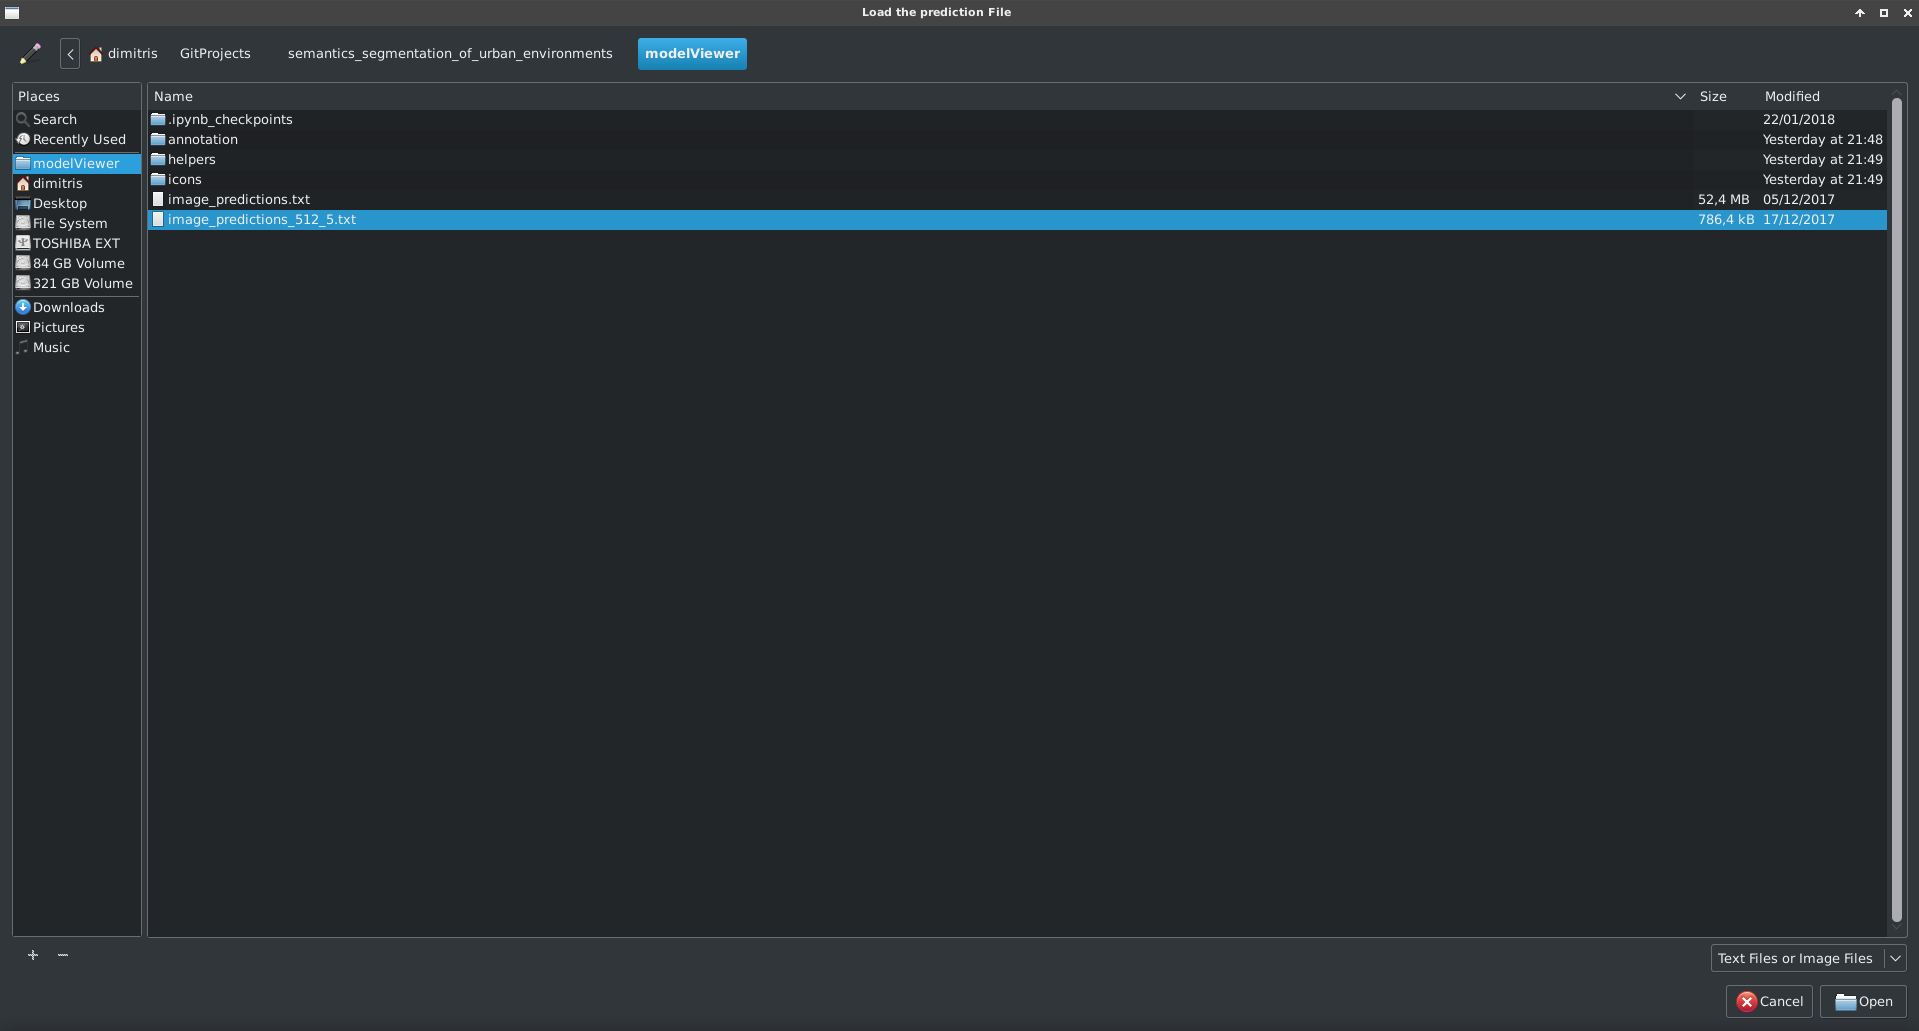
\includegraphics[width=\textwidth, scale=0.3]{Images/viewer_2}
\caption[\textgreek{Επιλογή Αρχείου}]{\textgreek{Επιλογή αρχείου/εικόνας αποτελεσμάτων}}\label{fig:viewer_2}
\end{figure}

\textgreek{Η εικόνα με τις προβλέψεις ζωγραφίζεται πάνω από την εικόνα εισόδου, όπου κάθε κατηγορία αντικειμένων έχει ένα χρώμα που την αντιπροσωπεύει (εικόνες} \ref{fig:viewer_3}\textgreek{ και} \ref{fig:viewer_4}). \textgreek{Ο δείκτης ανάλογα με την θέση του δείχνει με άσπρα έντονα γράμματα στα δεξιά του δείκτη την κατηγορία που ανήκει το εικονοστοιχείο. Επίσης, έχουμε δώσει την εξής λειτουργία, την ρυθμιζόμενη διαφάνεια του στρώματος με τις προβλέψεις για να δώσουμε την ευχέρεια στον χρήστη να επιλέξει την κατάλληλη επιθυμητή διαφάνεια ώστε να μπορεί να διακρίνει ευκολότερα τα αντικείμενα με τις αντίστοιχες κατηγορίες που ανήκουν.}

\begin{figure}[H]
 \centering
 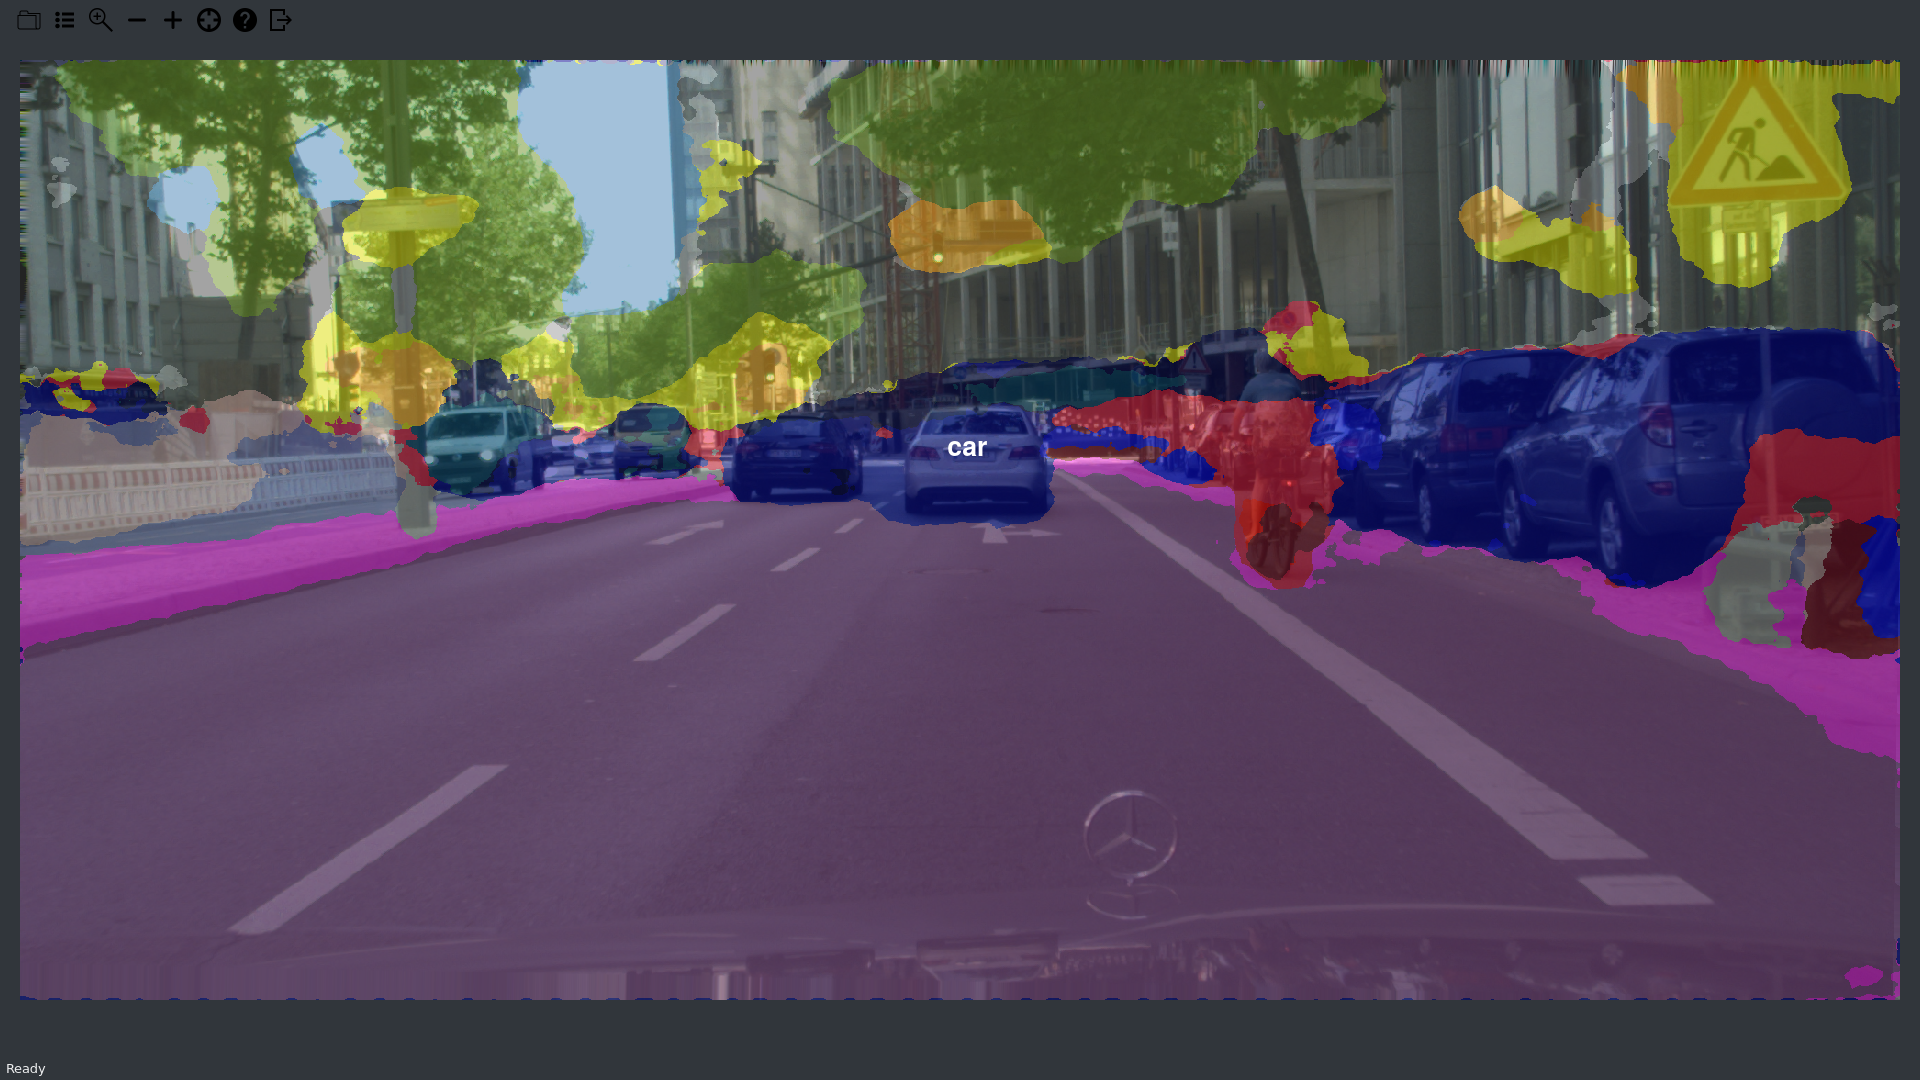
\includegraphics[width=\textwidth, scale=0.3]{Images/viewer_3}
\caption[\textgreek{Προβολή Ετικέτας}]{\textgreek{Προβολή εικόνας και πρόβλεψης του μοντέλου} .}
 \label{fig:viewer_3}
\end{figure}

\begin{figure}[H]
 \centering
 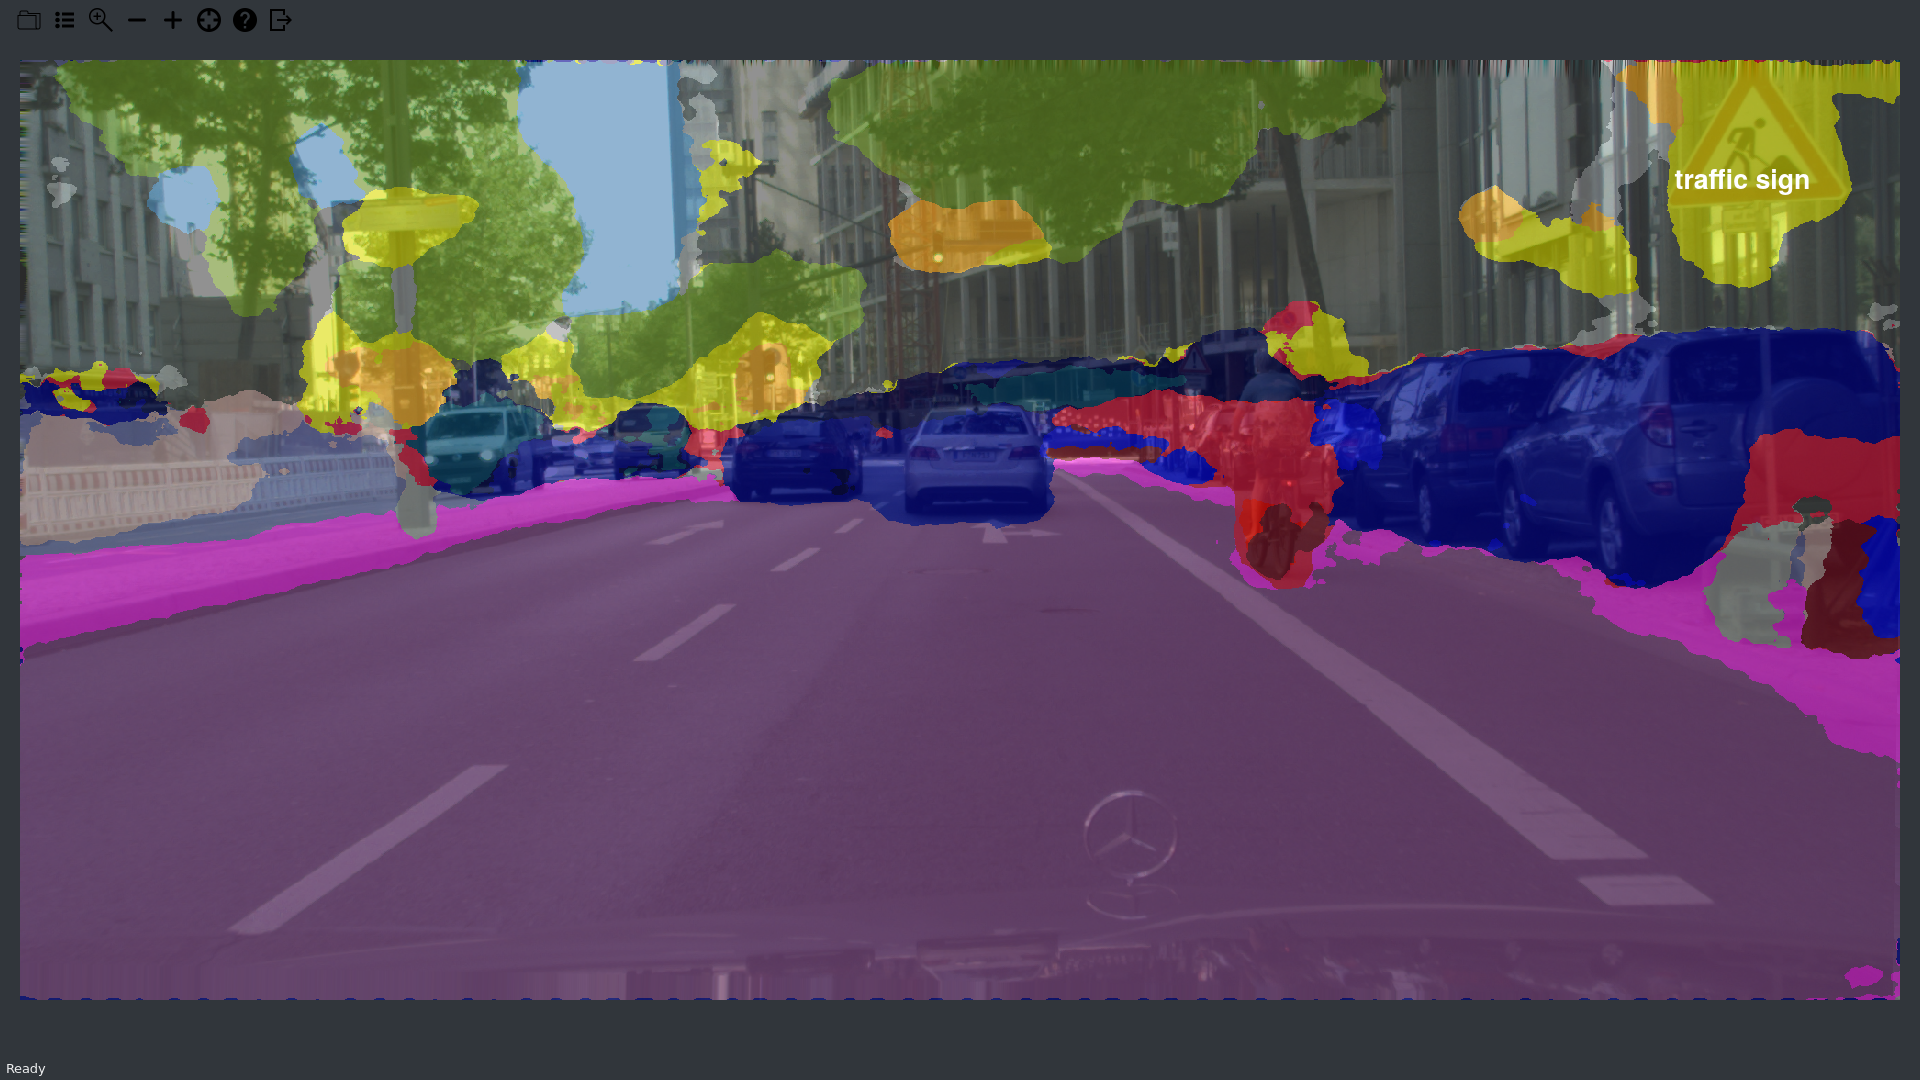
\includegraphics[width=\textwidth, scale=0.3]{Images/viewer_4}
\caption[\textgreek{Παράδειγμα Διαφάνειας}]{\textgreek{Παράδειγμα απεικόνισης ετικέτας σε επιλεγμένο βαθμό διαφάνειας.}}
 \label{fig:viewer_4}
\end{figure}

\textgreek{Τέλος, υπάρχει η δυνατότητα της μεγέθυνσης συγκεκριμένης επιφάνειας της εικόνας στατικού μεγέθους ανάλογα με την θέση που βρίσκεται ο δείκτης από το ποντίκι, δείχνοντας την ετικέτα του κεντρικού εικονοστοιχείου (εικόνα }\ref{fig:viewer_5}).

\begin{figure}[H]
 \centering
 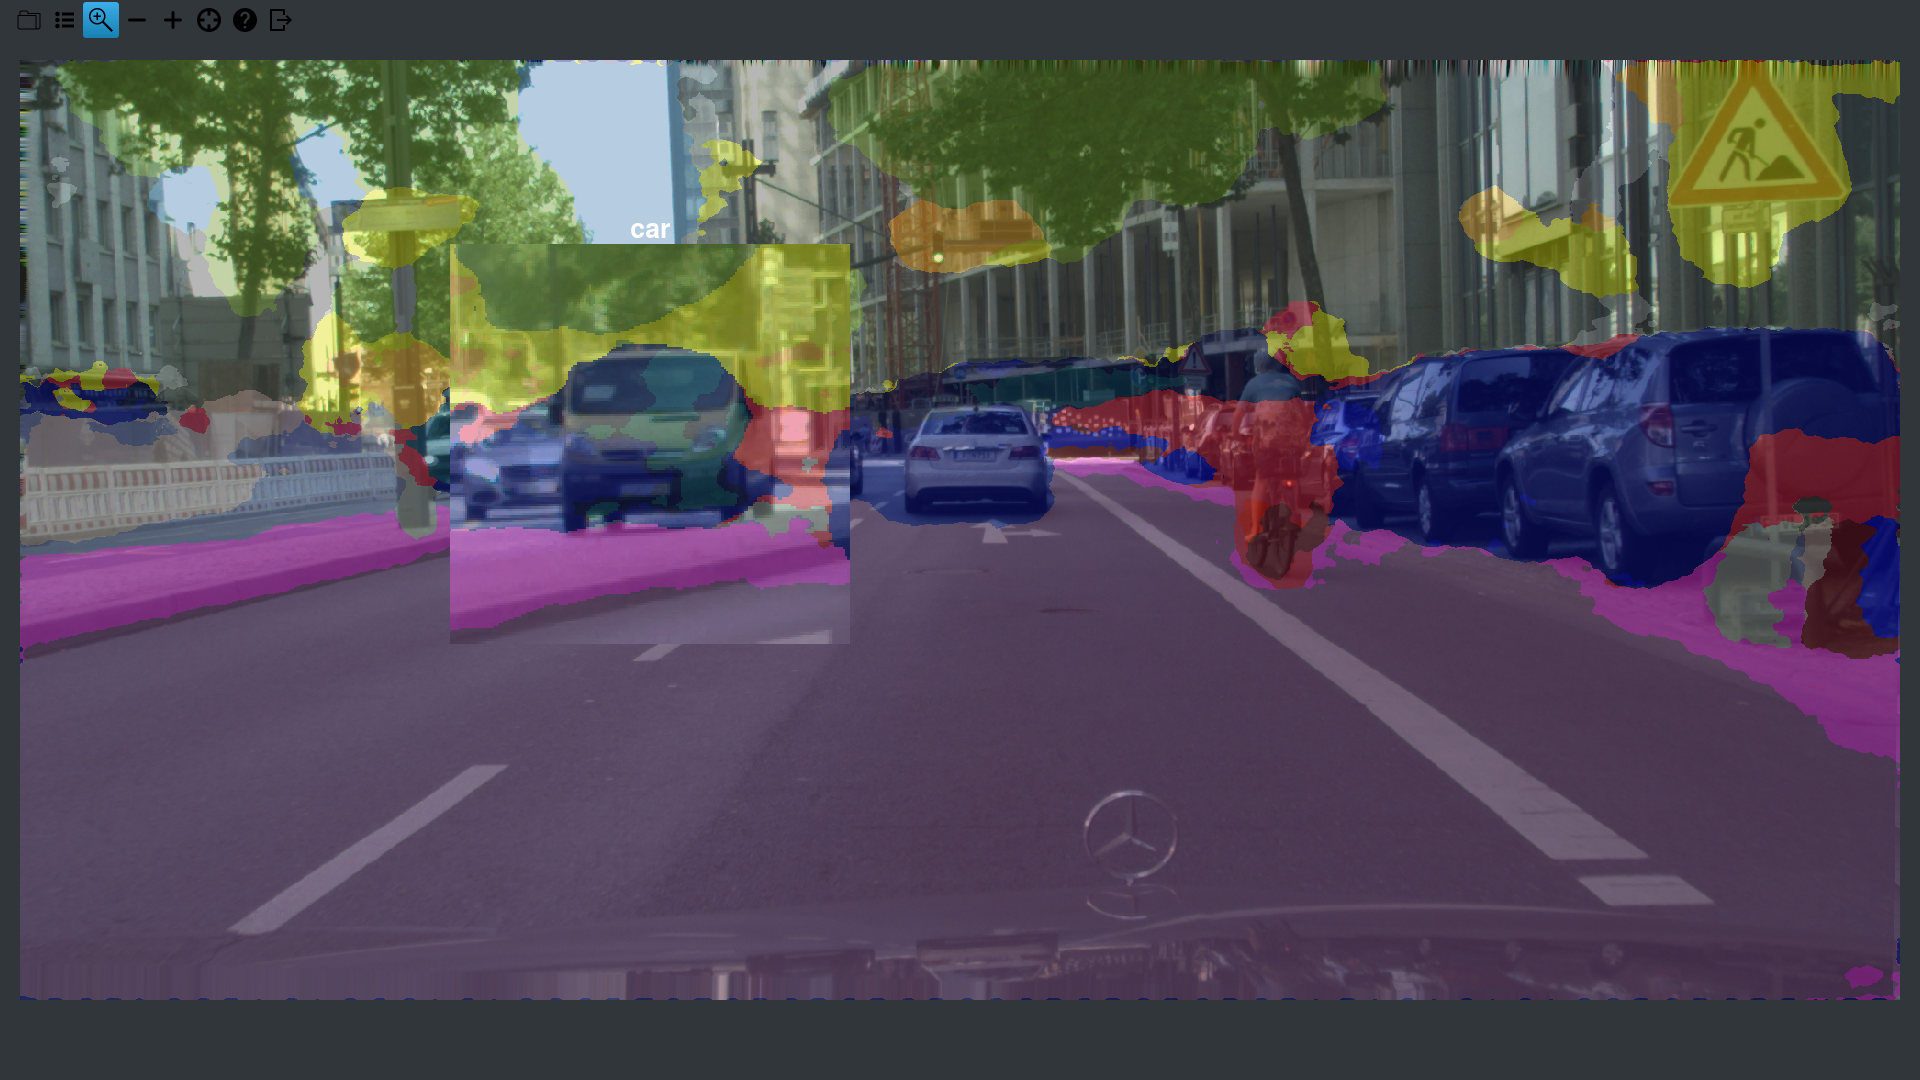
\includegraphics[width=\textwidth, scale=0.3]{Images/viewer_5}
\caption[\textgreek{Παράδειγμα της Λειτουργίας Μεγέθυνσης}]{\textgreek{Λειτουργία μεγέθυνσης επιφάνειας.}}
 \label{fig:viewer_5}
\end{figure}


\addtocontents{toc}{\protect\contentsline{chapter}{\protect\numberline{}\textgreek{Παράρτημα Α}}{}{chapter*.\thepage}}
%\addtocontents{toc}{\protect\contentsline{chapter}{\protect\numberline{}\textgreek{Παράρτημα Β}}{}{chapter*.\thepage}}

    %\newpage
    %\chapter{Introduction}

    \medskip
    \bibliography{thesis}
    
    %\printindex

\end{document}
